%%%%%%%%%%%%%%%%%%%%%%%%%%%%%%%%%%%%%%%%%%%%%%%%%%%%%%%%%%%%%%%%%%%%%%%%%
%%
%%  D I S S E R T A T I O N
%%
%%  Sergio A. de Carvalho Jr.
%%
%%%%%%%%%%%%%%%%%%%%%%%%%%%%%%%%%%%%%%%%%%%%%%%%%%%%%%%%%%%%%%%%%%%%%%%%%
\documentclass[12pt,pagesize,a4paper,BCOR1cm,DIV13,headsepline,cleardoubleplain,chapterprefix,halfparskip,pointlessnumbers,tablecaptionabove]{scrbook}
\usepackage{setspace}
\usepackage{amsmath,amssymb,amsthm,amsfonts}
\usepackage{latexsym}
\usepackage[american]{babel} 
\usepackage[round]{natbib}
\usepackage{longtable}
\usepackage{graphicx}\graphicspath{{./figures/}}
\usepackage{url}
\usepackage{bbm}
\usepackage{float}

%%%%%%%%%%%%%%%%%%%%%%%%%%%%%%%%%%%%%%%%%%%%%%%%%%%%%%%%%%%%%%%%%%%%%%%%%
% Further document formatting instructions
%%%%%%%%%%%%%%%%%%%%%%%%%%%%%%%%%%%%%%%%%%%%%%%%%%%%%%%%%%%%%%%%%%%%%%%%%
\setcapindent{1em}
\addtokomafont{caption}{\small}
\setkomafont{captionlabel}{\sffamily\bfseries}

%%%%%%%%%%%%%%%%%%%%%%%%%%%%%%%%%%%%%%%%%%%%%%%%%%%%%%%%%%%%%%%%%%%%%%%%%
% New environments and commands; hyphenation exceptions
%%%%%%%%%%%%%%%%%%%%%%%%%%%%%%%%%%%%%%%%%%%%%%%%%%%%%%%%%%%%%%%%%%%%%%%%%
%%%%%%%%%%%%%%%%%%%%%%%%%%%%%%%%%%%%%%%%%%%%%%%%%%%%%%%%%%%%%%%%%%%%%%
%% A hyphen that allows further hyphenation of a word
%%%%%%%%%%%%%%%%%%%%%%%%%%%%%%%%%%%%%%%%%%%%%%%%%%%%%%%%%%%%%%%%%%%%%%
\def\hyph{-\penalty0\hskip0pt\relax}

%%%%%%%%%%%%%%%%%%%%%%%%%%%%%%%%%%%%%%%%%%%%%%%%%%%%%%%%%%%%%%%%%%%%%%
%% Algorithm names
%%%%%%%%%%%%%%%%%%%%%%%%%%%%%%%%%%%%%%%%%%%%%%%%%%%%%%%%%%%%%%%%%%%%%%
\newcommand{\Greedyplus}{Greedy+}

%%%%%%%%%%%%%%%%%%%%%%%%%%%%%%%%%%%%%%%%%%%%%%%%%%%%%%%%%%%%%%%%%%%%%%
%% AMS definitions
%%%%%%%%%%%%%%%%%%%%%%%%%%%%%%%%%%%%%%%%%%%%%%%%%%%%%%%%%%%%%%%%%%%%%%
\theoremstyle{definition}
\newtheorem{problem}{Problem}
\newtheorem{definition}{Definition}[chapter]
\newtheorem{claim}[definition]{Claim}
\newtheorem{example}[definition]{Example}
\newtheorem{corollary}[definition]{Corollary}

\theoremstyle{plain}
\newtheorem{lemma}[definition]{Lemma}
\newtheorem{theorem}[definition]{Theorem}

%%%%%%%%%%%%%%%%%%%%%%%%%%%%%%%%%%%%%%%%%%%%%%%%%%%%%%%%%%%%%%%%%%%%%%
%% Float for displaying algorithms
%%%%%%%%%%%%%%%%%%%%%%%%%%%%%%%%%%%%%%%%%%%%%%%%%%%%%%%%%%%%%%%%%%%%%%
\floatstyle{ruled}
\floatname{algorithm}{Algorithm}
\newfloat{algorithm}{t}{}

%%%%%%%%%%%%%%%%%%%%%%%%%%%%%%%%%%%%%%%%%%%%%%%%%%%%%%%%%%%%%%%%%%%%%%%%%
% New commands
%%%%%%%%%%%%%%%%%%%%%%%%%%%%%%%%%%%%%%%%%%%%%%%%%%%%%%%%%%%%%%%%%%%%%%%%%

% Ignore, forcebreak, ...
\newcommand{\ignore}[1]{}
\newcommand{\forcebreak}{\nopagebreak\mbox{ }\\[-3ex]\nopagebreak}
\newcommand{\eop}{\hfill$\bullet$}

% Sets
\newcommand{\setR}{\mathbb{R}}

% Nucleotides
\newcommand{\DNA}{\text{DNA}}
\newcommand{\RNA}{\text{RNA}}
\newcommand{\tA}{\text{\ttfamily A}}
\newcommand{\tC}{\text{\ttfamily C}}
\newcommand{\tG}{\text{\ttfamily G}}
\newcommand{\tN}{\text{\ttfamily N}}
\newcommand{\tT}{\text{\ttfamily T}}
\newcommand{\tU}{\text{\ttfamily U}}
\newcommand{\NucA}{\text{\ttfamily A}}
\newcommand{\NucC}{\text{\ttfamily C}}
\newcommand{\NucG}{\text{\ttfamily G}}
\newcommand{\NucN}{\text{\ttfamily N}}
\newcommand{\NucT}{\text{\ttfamily T}}
\newcommand{\NucU}{\text{\ttfamily U}}
\newcommand{\NucX}{\text{\ttfamily X}}
\newcommand{\Nucs}[1]{{\tt{#1}}}
\newcommand{\emptyseq}{\epsilon}
\newcommand{\sep}{\text{\ttfamily \$}}
\newcommand{\wild}{\text{\ttfamily X}}
\newcommand{\SigmaX}{(\Sigma\cup\{\wild\})}

% Probability
\newcommand{\Erw}{\mathbb{E}}
\newcommand{\Var}{\text{Var}}
\newcommand{\R}{\mathbb{R}}
\newcommand{\Prob}{\mathbb{P}}
\newcommand{\Probhat}{\hat{\mathbb{P}}}
%%\newcommand{\Ind}[1]{\ensuremath{{\mathbb{I}}_{\{#1\}} }}
\newcommand{\Ind}[1]{\mathbbm{1}_{\{{#1}\}}}
\newcommand{\Eins}{{\mathbb{I}}}
\newcommand{\given}{\,|\,}

% Cal Letters
\newcommand{\CalA}{{\mathcal{A}}}
\newcommand{\CalB}{{\mathcal{B}}}
\newcommand{\CalC}{{\mathcal{C}}}
\newcommand{\CalD}{{\mathcal{D}}}
\newcommand{\CalE}{{\mathcal{E}}}
\newcommand{\CalF}{{\mathcal{F}}}
\newcommand{\CalG}{{\mathcal{G}}}
\newcommand{\CalL}{{\mathcal{L}}}
\newcommand{\CalM}{{\mathcal{M}}}
\newcommand{\CalN}{{\mathcal{N}}}
\newcommand{\CalP}{{\mathcal{P}}}
\newcommand{\CalQ}{{\mathcal{Q}}}
\newcommand{\CalS}{{\mathcal{S}}}
\newcommand{\CalT}{{\mathcal{T}}}
\newcommand{\CalU}{{\mathcal{U}}}
\newcommand{\CalX}{{\mathcal{X}}}
\newcommand{\CalY}{{\mathcal{Y}}}

% Algorithms
\newcommand{\aname}[1]{\textsc{#1}}
\newcommand{\atab}{\makebox[6ex]{}}
\newcommand{\MFOLD}{\aname{Mfold}}

% Binomial-like coefficients
\newcommand{\schoose}[2]{{\genfrac{(}{)}{0pt}{}{{#1}}{{#2}}}}
\newcommand{\ssubset}[2]{{\genfrac{\{}{\}}{0pt}{}{{#1}}{{#2}}}}
\newcommand{\scycle}[2]{{\genfrac{[}{]}{0pt}{}{{#1}}{{#2}}}}
\newcommand{\falling}[2]{{{#1}^{\underline{#2}}}}

% Other Math
\newcommand{\mathand}{{\text{ and }}}
\newcommand{\diag}{{\text{diag}}}
\newcommand{\N}{{\mathbb{N}}}

\newcommand{\eps}{\varepsilon}
\newcommand{\sig}{\varsigma}
\newcommand{\vphi}{\varphi}
\newcommand{\valpha}{{\underline{\alpha}}}
\newcommand{\vbeta}{{\underline{\beta}}}

% Bars and Hats
\newcommand{\betabar}{{\overline{\beta}}}
\newcommand{\lambdabar}{{\overline{\lambda}}}
\newcommand{\nbar}{{\overline{n}}}
\newcommand{\Thetabar}{\ensuremath{\overline{\Theta}}}
\newcommand{\Bbar}{{\overline{B}}}
\newcommand{\Ubar}{{\overline{U}}}
\newcommand{\ubar}{{\overline{u}}}
\newcommand{\vbar}{{\overline{v}}}
\newcommand{\xbar}{\ensuremath{\overline{x}}}
\newcommand{\Xbar}{\ensuremath{\overline{X}}}
\newcommand{\ybar}{{\overline{y}}}
\newcommand{\Phihat}{{\ensuremath{\hat{\Phi}}}}

%% (R)
%% \newcommand{\textR}{${}^\text{\textregistered}$}
\newcommand{\textR}{\raisebox{.6ex}{\scriptsize \textregistered}}

%% Na+, TM, *C, A, differential d.
\newcommand{\Naplus}{{\ensuremath{\text{Na}^+}}}
\newcommand{\TM}{T_\text{M}}
\newcommand{\degC}{\ensuremath{{}^\circ\text{C}}}
\newcommand{\Angstrom}{\text{\AA}}
\newcommand{\diff}{\,\text{d}}
\newcommand{\Dstd}[1]{\Delta{#1}^\circ}
\newcommand{\stdm}[1]{{#1}^\circ_\text{m}}
\newcommand{\Drstd}[1]{\Delta_\text{r}{#1}^\circ}
\newcommand{\Dr}[1]{\Delta_\text{r}{#1}}
\newcommand{\conceq}[1]{[{#1}]_\text{eq}}
\newcommand{\fd}[1]{$5'$-\Nucs{#1}-$3'$}
\newcommand{\rfd}[1]{r($5'$-\Nucs{#1}-$3'$)}
\newcommand{\dfd}[1]{d($5'$-\Nucs{#1}-$3'$)}

%% Strings, lcf and so on 
\newcommand{\substring}{\lhd}
\newcommand{\suf}[2]{{#1}_{(#2)}}

\newcommand{\lcf}{\ensuremath{\text{\upshape lcf}}}
\newcommand{\lcfe}{\ensuremath{\text{\upshape lcf}^1}}
\newcommand{\lcfvec}{\ensuremath{\text{\upshape LCF}}}
\newcommand{\lcfstat}{\ensuremath{\text{\upshape LCFS}}}

\newcommand{\lcpr}{\text{lcp}}  %% lcpr = lcp in roman font

\newcommand{\ms}{\text{\upshape ms}}
\newcommand{\mse}{\text{\upshape ms}^1}

\newcommand{\Romin}{{R^0_{\min}}}
\newcommand{\Remin}{{R^1_{\min}}}
\newcommand{\Rmax}{{R_{\max}}}

\newcommand{\pos}{\text{\upshape\ttfamily pos}}
\newcommand{\rank}{\text{\upshape\ttfamily rank}}
\newcommand{\cl}{\text{\upshape\ttfamily cl}}
\newcommand{\bck}{\text{\upshape\ttfamily bck}}
\newcommand{\lcp}{\text{\upshape\ttfamily lcp}}
\newcommand{\MS}{\text{\upshape\ttfamily MS}}
\newcommand{\MSe}{{\text{\upshape\ttfamily MS}^1}}
\newcommand{\qcode}[1]{\langle{#1}\rangle}

\newcommand{\csms}{\text{\upshape csms}}
\newcommand{\CSMS}{{\text{\upshape\ttfamily CSMS}}}

\newcommand{\Lo}{{L^\circ}}

%% Other Stuff
\newcommand{\steep}{\text{\textit{drop}}}
\newcommand{\clust}{\mathcal{B}}

%% Matrices
\newcommand{\cond}{\ensuremath{\text{\upshape cond}}}
\newcommand{\Rank}{\ensuremath{\text{\upshape rank}}}
\newcommand{\scond}{\ensuremath{\text{\upshape cond}_\text{\upshape{s}}}}
\newcommand{\tp}{\ensuremath{{}^\text{\sffamily\upshape T}}}
\newcommand{\MR}[2]{\ensuremath{\setR^{{#1}\times{#2}}}}
\newcommand{\Id}[1]{\ensuremath{\text{\upshape I}}_{#1}}
\newcommand{\eqmin}{\ensuremath{\simeq}}
\newcommand{\nm}[1]{\ensuremath{\| {#1} \|}}
\newcommand{\expm}{\ensuremath{\text{\upshape expm}}}

%% NonUnique
\newcommand{\mcov}{\mathcal{M}}
\newcommand{\acov}{\mathcal{A}}
\newcommand{\cmin}{\gamma}
\newcommand{\hmin}{\sigma}
\newcommand{\SDiff}[2]{{#1}\Delta{#2}}
\newcommand{\Separate}{\text{\textsc{Separate}}}
\newcommand{\ddpvec}{\begin{pmatrix}\delta\\\delta^+\end{pmatrix}}
\newcommand{\ddpvectp}{\begin{pmatrix}\delta\\\delta^+\end{pmatrix}^\text{\sffamily\upshape T}}
\newcommand{\hhpvec}[1]{\begin{pmatrix}h_{#1}\\h^+_{#1}\end{pmatrix}}
\newcommand{\zzpvec}[1]{\begin{pmatrix}z^{#1}\\z^{+,{#1}}\end{pmatrix}}

\hyphenation{phyco-erythrin strept-avidin oligo-nu-cleo-tide
Af-fy-met-rix tran-script hy-bri-di-za-tion cRNAs cRNA}

%%%%%%%%%%%%%%%%%%%%%%%%%%%%%%%%%%%%%%%%%%%%%%%%%%%%%%%%%%%%%%%%%%%%%%%%%
% Date handed-in
%%%%%%%%%%%%%%%%%%%%%%%%%%%%%%%%%%%%%%%%%%%%%%%%%%%%%%%%%%%%%%%%%%%%%%%%%
\newcommand{\abgabemonat}{Februar~2007}
\newcommand{\handinmonth}{February~2007}

%%%%%%%%%%%%%%%%%%%%%%%%%%%%%%%%%%%%%%%%%%%%%%%%%%%%%%%%%%%%%%%%%%%%%%%%%
% Beginning of document
%%%%%%%%%%%%%%%%%%%%%%%%%%%%%%%%%%%%%%%%%%%%%%%%%%%%%%%%%%%%%%%%%%%%%%%%%
\begin{document}
\selectlanguage{\american}
\frontmatter\pagestyle{plain}

%%%%%%%%%%%%%%%%%%%%%%%%%%%%%%%%%%%%%%%%%%%%%%%%%%%%%%%%%%%%%%%%%%%%%%%%%
%% Title pages
%%%%%%%%%%%%%%%%%%%%%%%%%%%%%%%%%%%%%%%%%%%%%%%%%%%%%%%%%%%%%%%%%%%%%%%%%
\title{Algorithms for Improving the Design and Production of
  Oligonucleotide Microarrays}
\author{S\'ergio Anibal de Carvalho Junior}
\date{\abgabemonat}
\publishers{\large{
  Dissertation\\
  zur Erlangung des akademischen Grades\\
  eines Doktors der Naturwissenschaften\\
  (Doctor rerum naturalium)\\
  ~\\
  an der Technischen Fakult\"at\\
  der Universit\"at Bielefeld\\
  ~\\
  ~\\
  Betreuer:\\
  Dr.~rer.~nat.~Sven Rahmann\\
  Prof.~Dr.~rer.~nat.~Jens Stoye\\
  ~\\
}}
%\lowertitleback{
%  1. Referee: Prof.~Dr.~Jens~Stoye\\
%  2. Referee: Dr.~Sven~Rahmann\\[2ex]
%}
%% \dedication{}
\maketitle[-1]

%%%%%%%%%%%%%%%%%%%%%%%%%%%%%%%%%%%%%%%%%%%%%%%%%%%%%%%%%%%%%%%%%%%%%%%%%
%% Front matter
%%%%%%%%%%%%%%%%%%%%%%%%%%%%%%%%%%%%%%%%%%%%%%%%%%%%%%%%%%%%%%%%%%%%%%%%%
\clearpage
\setcounter{tocdepth}{1}
%%\listoffigures
%%\listoftables
%%%%%%%%%%%%%%%%%%%%%%%%%%%%%%%%%%%%%%%%%%%%%%%%%%%%%%%%%%%%%%%%%%%%%%%%%%%%%%%%
\chapter*{Foreword}
\addcontentsline{toc}{chapter}{Foreword}
%%%%%%%%%%%%%%%%%%%%%%%%%%%%%%%%%%%%%%%%%%%%%%%%%%%%%%%%%%%%%%%%%%%%%%%%%%%%%%%%

Microarrays are a ubiquitous tool in molecular biology with a wide range of
applications on a whole-genome scale including high-throughput gene expression
analysis, genotyping, and resequencing.

Several different microarray platforms exist, but this thesis focuses on
high-density oligonucleotide arrays. The advantage of higher densities arrays
is that they allow, for instance, the simultaneous measurement of the expression
of several thousand genes at once.

High-density microarrays are usually produced by light-directed combinatorial
chemistry that builds the probe sequences base-by-base. Because of the natural
properties of light, the quality of a microarray can be improved by carefully
designing the physical arrangement, or \emph{layout}, of its probes.

In this thesis, we review models for evaluating the layout of oligonucleotide
microarrays and survey algorithmic approaches that can be used in their design.

%% What follows is from Sven's thesis: use it as a template

DNA chips allow to quickly obtain and compare gene expression profiles
of different cell or tissue samples. As one of many applications, one
hopes to better understand various types and subtypes of cancer and to
improve cancer therapy by characterizing the differences between
the expression profiles of healthy cells and tumor cells.

The first chapter of this thesis offers an overview of existing
microarray technologies and contrasts them with other techniques for
gene expression analysis. High-density oligonucleotide arrays are
described in detail.

Gene expression analysis with DNA chips is a high-throughput technique
that produces massive amounts of data; however, this technique is not
error-free. Each step of an experiment must be performed carefully. In
particular, the DNA chip must be carefully designed and manufactured.
This thesis proposes and describes solutions for some of the
algorithmic problems that arise in this phase. These problems are
formulated in detail in the last section of Chapter x.

My research started with the general question of how to find
oligonucleotide probes for highly homologous transcripts when it
cannot be guaranteed that a sufficiently large set of clearly
transcript-specific (or \emph{unique}) probes can be found. An
interesting future large-scale application could be the individual
expression measurement of all splice variations of all genes in the
human genome, for example. The basic idea was to find several
\emph{non-unique} probes such that different probes hybridize to
different combinations of targets, with the hope that the measured
signal can then be decoded into the individual expression levels. Two
question then follow immediately: How does the decoding work, and how
can the probes be designed in a way that makes the decoding as simple
as possible?

In early 2001, custom probe design was in its infancy. The design of
the large commercial chips, such as the Affymetrix GeneChip\textR, was
a well guarded secret of the respective companies. Several other
research groups were also beginning to work on probe selection, and
their results, made the
problem more popular.  I soon realized that, before actually working
on non-unique probes, more fundamental questions should be addressed.
A high-performance large-scale probe selection system for unique
probes would be very useful but did not exist. Such a system could
then be used as a basis for non-unique probe design. These
considerations are reflected in this thesis.

Once a set of probes is chosen for a chip design, the chip must be
produced. With several technologies, such as the Affymetrix
GeneChip\textR\ arrays and febit's {\sffamily geniom}\textR\ 
{\sffamily one} system, the probes are synthesized in situ on the chip
with a combination of photolithography and combinatorial chemistry.
We consider the problem of optimizing the nucleotide deposition
sequence to lower production costs and to decrease the overall error
rate during synthesis.

A concluding discussion about the results of this thesis and an
outlook into the future can be found in Chapter~\ref{ch:discussion}.

\paragraph{Publications.}
Parts of this thesis have been published in advance.

This thesis also contains previously unpublished material, namely
\begin{itemize}
\item new placement algorithm that simultaneously places and re-embeds
  the probes
\end{itemize}

\paragraph{Acknowledgments.}
This work was carried out while I was at the...
It has been a very enjoyable experience, thanks to all present and
former colleagues and students in the Bioinformatics program.

I would especially like to thank Sven Rahmann for suggesting the
topic, providing initial ideas, and for the opportunity to write this
thesis under his guidance.

The support of the whole computer service group at the CeBiTec was
crucial to the success of this work, and I cannot thank them enough
for their help.

I enjoyed fruitful discussions with many people while this thesis was
underway; in particular, I am grateful to ...
for their valuable hints and comments. 

... read early drafts of several chapters of this thesis and
helped to improve it in many ways through their comments.

I would like to thank Dr. Peter Hahn and Chris MacPhee who worked on several QAP instances
derived from artificial microarray chips for their efforts.

\ignore{
Last but not least, I thank Karla Aleluia de Carvalho for her love and
patience while I was writing this thesis. Heartfelt thanks also go to
my parents and the rest of the family.}

\vspace*{6ex}
S\'ergio A. de Carvalho Jr.\hfill Bielefeld, \handindate

%%%%%%%%%%%%%%%%%%%%%%%%%%%%%%%%%%%%%%%%%%%%%%%%%%%%%%%%%%%%%%%%%%%%%%%%%%%%%%%%%%
\chapter*{Danke sch\"on!}
\addcontentsline{toc}{chapter}{Danke sch\"on!}
%%%%%%%%%%%%%%%%%%%%%%%%%%%%%%%%%%%%%%%%%%%%%%%%%%%%%%%%%%%%%%%%%%%%%%%%%%%%%%%%

Danke sch\"on!

\ignore{
Last but not least, I thank my wife Karla for her love, support and
patience during the last three years. Heartfelt thanks also go to
my parents and the rest of the family.}

%%\chapter{Abbreviations and Notation}
\label{ch:notation}

%% %%%%%%%%%%%%%%%%%%%%%%%%%%%%%%%%%%%%%%%%%%%%%%%%%%%%%%%%%%%%%%%%%%%%%%%%%%%%%
%% Notation
%% --------
%%
%% n: number of probes
%% m: number of spots
%% t: step index
%% N: deposition sequence
%% N_t: nucleotide added at step t
%% M_t: mask of step t
%% T: total number of synthesis steps
%%
%% s,s': spot indices
%% p_k: probe sequence of probe with index k
%% k(s): probe index for spot s
%% \eps_k: embedding vector for probe with index k
%% \eps_{k(s)}: embedding vector at spot s
%%
%% \mathcal{B}_t: border length of mask M_t
%%
%% For the QAP formulation (not here!)
%% k,l: indices for probes
%% i,j: indices for spots
%%
%% %%%%%%%%%%%%%%%%%%%%%%%%%%%%%%%%%%%%%%%%%%%%%%%%%%%%%%%%%%%%%%%%%%%%%%%%%%%%%

%%
%% See also
%% http://www.mcponline.org/glossary/
%%
\small
\vspace*{-4ex}
\subsection*{Abbreviations in alphabetical order}
\begin{longtable}[l]{rl}
\endfirsthead\endhead\endfoot\endlastfoot
%%
%% A
A, \tA    & adenine\\
\Angstrom   & Angstrom; $1\Angstrom = 10^{-10}\text{ m}=1/10 \text{ nm}$\\
aRNA        & anti-sense RNA, amplified RNA; complementary to mRNA\\
%%
%% B
bp          & base pair(s)\\
%%
%% C
C, \tC    & cytosine\\
\degC       & degrees centigrade (Celsius)\\
cDNA        & complementary DNA; DNA synthesized from mRNA by RT\\
CDS         & coding sequence\\
cRNA        & complementary RNA; same as aRNA\\
CSMS, csms  & cumulative statistics of matching statistics\\
Cy3         & Cyanine 3-dNTP; in fluorescently labeled DNA\\
Cy5         & Cyanine 5-dNTP; in fluorescently labeled DNA\\
%%
%% D
DMD         & digital micromirror device\\
DNA         & deoxyribonucleic acid\\
dN          & any deoxynucleotide; any of dA, dC, dG, dT\\
dNTP        & any deoxynucleotide-triphosphate; 
                any of dATP, dCTP, dGTP, dTTP\\
%%
%% E
EST         & expressed sequence tag\\ 
%%
%% G
G, \tG    & guanine\\
%%
%% H
HPLC        &  high-pressure liquid chromatography\\
%%
%% I
IVT         & in-vitro transcription\\
%% 
%% K
K           & Kelvin; physical unit of temperature\\
%%
%% L
LCF         & longest common factor\\
LCFS        & longest common factor statistics\\
%%
%% M
M           &  physical unit of molar concentration: 1 M = 1 mol/l\\
MCMC        &  Markov chain Monte Carlo\\
MES         &  2-(N-morpholino)ethanesulfonic acid\\
mol         &  physical unit of amount of substance\\
{}          &{\qquad}1 mol = as many entities as atoms in $0.012$ kg of carbon 12\\
mRNA        &  messenger RNA\\
MS, ms      &  matching statistics\\
%%
%% N
N, \tN    &  any of the bases A, C, G, T/U\\
{[\Naplus]} &  salt (sodium ion) concentration\\
NaCl        &  salt (sodium chloride)\\
NN          &  nearest neighbor\\
nt          &  nucleotide(s)\\
%%
%% O
oligo-(dT)  &  primer of 12--20 dTs binding to the poly(A) tail of 
                 eukaryotic mRNA\\
%%
%% P
P           &  phosphor\\
${}^{33}$P  &  a radioactive phosphor isotope\\
PAGE        &  polyacrylamide gel electrophoresis\\
PCR         &  polymerase chain reaction\\
PEM         &  percent of expected mutations (unit of evolutionary time)\\
%%
%% R
RNA         & ribonucleic acid\\
RT          & reverse transcription\\
RTase       & reverse transcriptase; an enzyme\\
RT-PCR      & reverse transcription-polymerase chain reaction\\
%%
%% S
SAGE        & serial analysis of gene expression\\
SAPE        & streptavidin phycoerythrin\\
SBH         & sequencing by hybridization\\
SCS         & shortest common supersequence\\
SCSP        & shortest common supersequence problem\\
SNP         & single nucleotide polymorphism\\
SSC         & saline sodium citrate buffer\\
SSPE        & saline sodium phosphate buffer\\
SVD         & singular value decomposition\\
%%----------------------------------------------
%% T
T, \tT    &  thymine\\
T7          &  a bacteriophage that infects \emph{E.\ coli};\\
{}          &{\qquad}these viral parasites are numbered T1 through T7\\
\textit{Taq}&  \textit{Thermus aquaticus}; a heat-resistant bacterium\\
TIFF        &  tagged image file format\\
transfrag   &  transcript fragment\\
tRNA        &  transfer RNA\\
%%----------------------------------------------
%% U 
U, \tU    &  uracil\\
UTR         &  untranslated region; part of mRNA transcripts\\
%%
%%
\end{longtable}


\subsection*{Notation by topic}
\newcommand{\ltchap}[1]{\multicolumn{2}{l}{\sffamily\textbf{Chapter~{#1}}}\\\nopagebreak}

Notation introduced in early chapters is also used in subsequent chapters.
\begin{longtable}[l]{rl}
\endfirsthead\endhead\endfoot\endlastfoot
%%
%% Chapter 1
\ltchap{1}
$p$      & probe sequence; a string\\
$|p|$    & length of $p$\\
$t$      & transcript or target sequence\\
$T$      & transcriptome $T=(t_1,\dots,t_n)$\\
$m$      & number of probes\\
$i$      & probe index\\
$n$      & number of transcripts\\
$j$      & transcript index\\
$\theta$ & hybridization conditions; parameters\\
$a(p,t;\theta)$ & affinity coefficient between $p$ and $t$, given $\theta$\\
$p\substring t$ & $p$ is a factor (substring) of $t$\\
$\eps$   & lower affinity limit for specific hybridization\\[2ex]
%%
%% Chapter 2
\ltchap{2}
$x=(x_j)$     & $n$-vector of transcript expression levels\\
$y=(y_i)$     & $m$-vector of measured probe signals\\
$A=(A_{ij})$  & $m\times n$-matrix of probe-transcript affinity coefficients; $y=A\cdot x$\\
$t(i)$        & index of the unique target that probe $i$ binds to\\
$a$, $a_i$    & particular affinity coefficients\\
$\rho_{ij}$   & position dependent factor of $A_{ij}$\\
$\beta_{ij}$  & hybridization stability dependent factor of $A_{ij}$\\
$\gamma_{ij}$ & sequence composition dependent factor of $A_{ij}$\\
$\sigma_{ij}$ & self-complementarity dependent factor of $A_{ij}$\\
$\eps_i$      & stochastic additive noise of probe signal intensity\\
$c_i$, $c$    & systematic additive offset of signal intensity\\
$\alpha$      & scale of signal intensity\\
$\eta_{ij}$   & stochastic multiplicative noise of signal intensity\\[1ex]
$\diff$       & differential operator\\
$\Delta$      & denotes a difference\\
$U$; $q$; $w$ & internal energy; heat; work\\
$p$           & pressure\\
$V$           & volume\\
$T$           & temperature\\
$H$; $\stdm{H}$; $\Drstd{H}$ & enthalpy; standard molar enthalpy; standard reaction enthalpy\\
$S$; $\stdm{S}$; $\Drstd{S}$ & entropy; standard molar entropy; standard reaction entropy\\
$G$; $\stdm{G}$              & Gibbs energy; standard molar Gibbs energy\\
$\Drstd{G}$; $\Dr{G}$        & standard Gibbs energy of reaction; reaction Gibbs energy\\
$\xi$         & extent of reaction\\
$R$           & gas constant; $R = 8.3145 \text{ J K$^{-1}$ mol$^{-1}$}$\\
$K$           & equilibrium constant\\
$\conceq{\text{S}_2}$ & equilibrium concentration of reactant $\text{S}_2$ (single stranded probes)\\
%%$\beta$       & hybridization probability, stability factor\\
$\TM$         & melting temperature\\[2ex]
%%
%% Chapter 3
\ltchap{3}
$\lcf(p,t)$      & length of the longest common factor of $p$ and $t$\\
$\lcfe(p,t)$     & same, allowing one mismatch\\
$\lcf^*(p,t)$    & combined measure derived from $\lcf$ and $\lcfe$\\
$\lcfvec(p\given T)$  & LCF vector of probe $p$ against transcriptome $T$\\
$\lcfstat(p\given T;\Delta)$  & LCF statistics of $p$ against $T$ of width $\Delta$\\
$\delta$         & index of LCF statistics, $0\leq\delta<\Delta$\\
& \atab difference between full probe length and LCF length\\
$T(i)$           & index set of intended targets for probe $i$\\
$T$              & transcriptome; see Chapter~1\\
$U'(p_i\given T)$& unspecificity of probe $i$ in $T$; formal definition\\
$\tau$           & temperature; to avoid confusion with transcriptome $T$\\
$\beta(\delta)$  & average hybridization probability as a function of $\delta$\\
$\zeta$          & offset constant; $\zeta=\ln(\beta(0)/(1-\beta(0)))$\\
$b>0$            & average Gibbs energy per base pair in units of $(R\tau)$\\
$u(\delta)$      & approximation to $\beta(\delta)$\\
$U(p_i\given T)$ & unspecificity of probe $i$ in $T$; practical definition\\[2ex]
%%
%% Chapter 4
\ltchap{4}
$T=(T_c)$           & transcriptome of transcript collections $T_c$ ($c=1..C$)\\
$C$                 & number of collections\\
$T_c = \{t_{c,j}\}$ & transcript collection $c$ with transcripts $t_{c,j}$ ($j=1..N_c)$\\
$N_c$               & number of transcripts in collection $c$\\
$s$                 & target sequence\\
$\Sigma$            & alphabet; here $\Sigma=\{\Nucs{A,C,G,T}\}$\\
$\Sigma^*$; $\Sigma^+$ & all strings (non-empty strings) over alphabet $\Sigma$\\
$\sep$              & string end marker and separator\\
$\tX$               & unspecified or wildcard character\\
$\pos$              & suffix array\\
$\lcpr(s,t)$        & length of the longest common prefix of $s$ and $t$\\
$\lcp$              & longest common prefix array\\
$q$                 & bucket prefix length\\
$\bck$              & bucket array\\
$\gamma=\qcode{Q}$  & numerical radix-$q$ representation of a $q$-gram $Q$\\
$\cl$               & collection number array\\
$\ms^{s|t}=(\ms^{s|t}_i)$ & matching statistics of $s$ against $t$\\
$\ms^{s|t;f}$       & matching statistics allowing $f$ mismatches of $s$ against $t$\\
$\Romin$            & minimum value of relevant matching statistics\\
$\Remin$            & minimum value of relevant ms.\ with one mismatch\\
$\Rmax$             & maximum value of relevant matching statistics\\
$\MS[i][c]$         & matching statistics array; $\MS[i][c]=\ms^{s|T_c}_i$\\[1ex]
%%
$(i,J)$             & jump at position $i$ to level $J$\\
$n,m$               & string lengths; $|s|=m$, $|t|=n$\\
$\Prob$             & generic notation for a probability measure\\
$\Erw$              & generic notation for an expectation\\
$\pi=(\pi_c)_{c\in\Sigma}$ & character distribution for a random sequence model\\
$p$                 & probability that two random characters match\\
$q$                 & $q:=1-p$\\
$K_L$               & random number of occurrences of a random $L$-gram in a string\\
$\rho_L$            & probability that a jump to level $L$ occurs at a fixed position\\
$E_L$               & expected number of jumps to level $L$ in matching statistics\\
$E^+_L$             & expected number of jumps to level $\geq L$ in matching statistics\\
$\Lo$               & center of the distribution of the LCF of two random strings\\[2ex]
%%
%% Chapter 5
\ltchap{5}
$d$      & probe distance from the transcript's $3'$-end\\
$p_i=(d_i,\ell_i)$ & probe $i$ defined by end distance $d_i$ and length $\ell_i$\\
$f(d)$; $f_i$ & position preference factor for distance $d$; $f_i:=f(d_i)$\\
$h_i$    & hairpin formation probability for probe $i$\\
$U_i$    & unspecificity for probe $i$\\
$B_i$    & badness value for probe $i$\\
$\CalB(\delta)$ & additional badness for probes clustering within distance $\delta$\\
$B'_i$; $\Bbar'$ & modified badness value for probe $i$; threshold $\Bbar'$\\
$S$           & selected probe set\\[2ex]
%%
%%
\ltchap{6}
$\Ind{\cdot}$ & generic notation for an indicator function\\
$S=(s_c)$     & target sequences for all collections $c=1,\dots,C$\\
$H=(H_{ij})$  & binary $m\times n$ hybridization matrix of probes vs.\ targets\\
$D$           & design, i.e. a selection of probes; $D\subset\{1,\dots,m\}$\\
$A^D$; $H^D$  & affinity and hybridization matrix restricted to rows from $D$\\
$\mcov$       & minimum target coverage\\
$\acov$       & average target coverage\\
$A\tp$        & transpose of $A$\\
$\Sigma$      & diagonal matrix with singular values $(\sigma_j)$ of $A$\\
$\sigma_j$    & $j$-th largest singular value\\
$\diag(\cdot)$& diagonal matrix with specified entries\\
$A^-$         & pseudo-inverse of $A$\\
$\|\cdot\|_2$ & Euclidean norm of a vector; spectral norm of a matrix\\
$\|\cdot\|_\infty$ & maximum norm of a vector\\
$\cond(A)$    & condition number of $A$\\
$\scond(A)$   & Skeel condition number of $A$\\
$\mu$         & maximal number of probes that may be selected\\[1ex]
%%
$S$,$T$       & sets of target indices\\
$S\Delta T$   & symmetric set difference of $S$ and $T$\\
$P(S)$        & set of probes that hybridize to any target in $S$\\
$T(i)$        & set of targets that hybridize to probe $i$\\
$\gamma$      & desired minimum target coverage\\
$\sigma$      & desired minimum target set separation\\
$\delta\in\{0,1\}^m$ & binary vector representation of design $D$\\
$h_j$         & $j$-th column of binary hybridization matrix $H$\\
$z^{S,T}=(z^{S,T}_i)$  & indicates whether probe $i$ separates sets $S$ and $T$\\
$\delta^+$, $h_j^+$, $z^+$ & vectors extended for virtual unique probes\\
$B$           & maximal size of target sets to be separated\\
$f_0$; $f_1$  & false negative (positive) error rate\\
$\Prob(x)$    & prior probability of binary expression vector $x\in\{0,1\}^n$\\
$\Prob(y\given x)$ & likelihood of probe signals $y\in\{0,1\}^m$, given $x$\\
$\pi(x) = \Prob(x\given y)$ & posterior probability of $x$ for fixed $y$\\
$q(z \given x)$ & proposal probability for new solution $z$ at current solution $x$\\
$\CalN(x)$      & neighborhood of $x$\\
$\alpha(x,z)$   & acceptance probability for $z$ at $x$\\[1ex]
%%
$Q$             & rate matrix of an evolutionary Markov process\\
$t$             & evolutionary time\\
$P^t$           & Markov transition kernel for time $t$\\
$\expm(Q)$      & matrix exponential; $\expm(Q):=\sum_{n\geq 0}\, Q^n/n!$\\[2ex]
%%
%% Chapter 7
\ltchap{7}
$\csms^{s|t}$   & cumulative statistics of matching statistics of $s$ against $t$\\
& \atab $\csms^{s|t}_{i,\mu}$ refers to position $i$ in $s$ and matches of length $\geq \mu$\\
$\CSMS[i][\mu]$ & CSMS array; $\CSMS[i][\mu]=\csms^{s|t}_{i,\mu}$ if $\mu\in[\Romin,\Rmax]$\\
$\sigma^i_{k,u}$& unexpected CSMS at offset $k$ for a probe starting at $i$\\
$L_{i,\delta}$  & whole genome surrogate for $\lcfstat(p_i)_\delta$\\[1ex]
$L$             & length of hypothetical transfrags\\
$D$             & distance between start points of hypothetical transfrags\\
$K$             & transfrags known to be present\\
$P_1$           & probes expected to show a signal because of $K$\\
$M$             & transfrags of unknown status; {$M=\{1..n\} \setminus K$}\\
$N$             & transfrags most likely not present\\
$J$             & transfrags whose status is inferred by sampling; $J=\{1..n\}\setminus(K\cup N)$\\
$\chi$          & fraction of transfrags hybridizing to additional probes\\[2ex]
%%
%% Chapter 8
\ltchap{8}
$\Sigma$    & DNA alphabet\\
$\pi$       & permutation of the nucleotides\\
$\CalS$     & sequence set\\
$e$         & binary embedding vector of a string into a supersequence\\
$E$         & embedding matrix with rows $e_i$, $i=1..|\CalS|$\\
$\CalU$     & upper bound on the supersequence length\\
$\CalL$     & lower bound on the supersequence length\\
$L_i$       & length of the $i$-th sequence in $\CalS$\\
$N_i(x)$    & number of occurrences of $x\in\Sigma$ in the $i$-th sequence\\
$N(x)$      & $\max_i\, N_i(x)$\\
$C_i$       & completion step of the $i$-th sequence\\
$W_{i,k}$   & number of unproductive steps between $(k-1)$-st and $k$-th productive\\&\atab step for sequence $i$\\
$\Phi$      & cumulative distribution function of the standard Normal distribution
\end{longtable}
\normalsize


\paragraph{Trademark Notice.} 
Affymetrix\textR\ and GeneChip\textR\ are registered trademarks of
Affy\-metrix, Inc., Santa Clara, CA, U.S.A.  The terms {\sffamily
  geniom}\textR\ {\sffamily one} and DNA processor\textR\ are
registered trademarks of febit AG, Mannheim, Germany.

\tableofcontents
\clearpage\pagestyle{headings}
\mainmatter

%%%%%%%%%%%%%%%%%%%%%%%%%%%%%%%%%%%%%%%%%%%%%%%%%%%%%%%%%%%%%%%%%%%%%%%%%
%% Main Text
%%%%%%%%%%%%%%%%%%%%%%%%%%%%%%%%%%%%%%%%%%%%%%%%%%%%%%%%%%%%%%%%%%%%%%%%%
%%%%%%%%%%%%%%%%%%%%%%%%%%%%%%%%%%%%%%%%%%%%%%%%%%%%%%%%%%%%%%%%%%%%%%%%%%%%%%%%
\chapter{Introduction}
\label{ch:intro}
%%%%%%%%%%%%%%%%%%%%%%%%%%%%%%%%%%%%%%%%%%%%%%%%%%%%%%%%%%%%%%%%%%%%%%%%%%%%%%%%

\section{DNA and Genes}
\label{sec:intro_genes}

Choose another title for this sub-section.

\section{Functional Genomics}
\label{sec:intro_funcgen}

Choose another title for this sub-section.

\section{High-density Oligonucleotide Microarrays}
\label{sec:intro_oligoarrays}

Oligonucleotide microarrays consist of short DNA fragments, called
\emph{probes}, affixed or synthesized at specific locations, called
\emph{features} or \emph{spots}, of a solid surface. Microarrays are
based on the principle of Watson-Crick base pairing. Each probe is a
single-stranded DNA molecule of 10 to 70 nucleotides that perfectly matches
with a specific part of a \emph{target} molecule. The probes are used to
verify whether (or in which quantity) the targets are present in a
given biological sample.

This type of microarray was originally designed in the late 1980s as a tool for
DNA sequencing, a technology that is known as DNA Sequencing by Hybridization.

The first step of a microarray experiment consists of collecting mRNAs
or genomic DNA from the cells or tissue under investigation. The mixture
to be analyzed is prepared with fluorescent tags and loaded on the array,
allowing
the targets to hybridize with the probes. Any unbound molecule is
washed away, leaving on the array only those molecules that have found
a complementary probe. Finally, the array is exposed to a light source
that induces fluorescence, and an optical scanner reads the intensity
of light emitted at each spot.

Under ideal conditions, each probe will hybridize only to its target.  Thus,
it is possible to infer whether a given molecule is present in the sample by
checking whether there is light coming from the corresponding spot of the
array.  The expression level of a gene in a cell can also be inferred because
each spot contains several million identical probes, and the strength of the
fluorescent signal on a spot is expected to be proportional to the
concentration of the target in the sample. In practice, each target is queried
by several probes (its \emph{probe set}), and complex statistical calculations
are performed to infer the concentration from the observed signals.

High-density microarrays, also called microarray chips, can have more than a
million spots, and are thus able to query tens of thousands of genes, covering
the entire genome of an organism.  The pioneering Affymetrix GeneChip\textR\ 
arrays, for instance, have up to 1.3~million spots on a coated quartz
substrate measuring a little over 1~cm$^2$.  The spots are as narrow as
5~$\mu$m (5~microns, or 0.005 mm), and are arranged in a regularly-spaced
rectangular grid.

\subsection{Oligonucleotide Microarray Production}

GeneChip arrays are produced by combinatorial chemistry and techniques derived
from micro-electronics and integrated circuits fabrication. Probes are typically
25 bases long and are synthesized on the chip, in parallel, in a series of
repetitive steps. Each step appends the same kind of nucleotide to probes of
selected
regions of the chip. The selection of which probes receive the nucleotide is
achieved by a process called \emph{photolithography} \citep{Fodor1991}.

\begin{figure}\centering
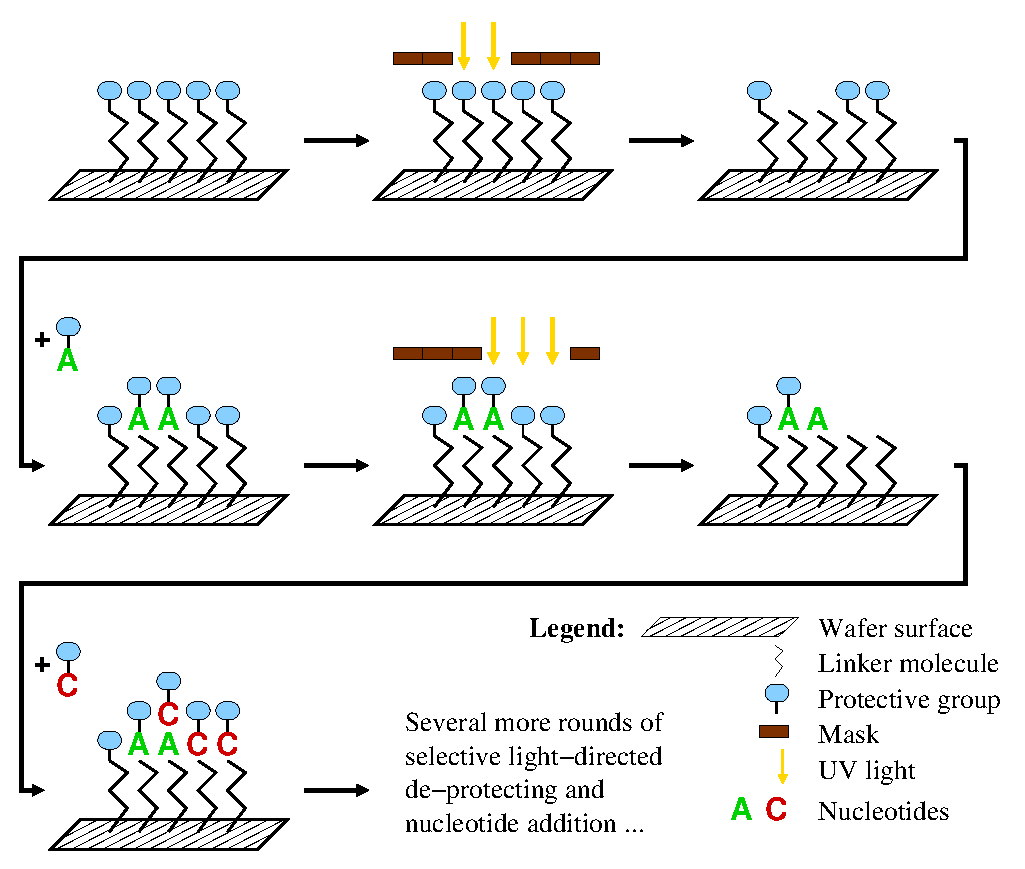
\includegraphics[width=.7\textwidth]{production.eps}
\caption{Affymetrix's probe synthesis via photolithographic masks. The chip is
  coated with a chemical compound and a light-sensitive protecting group;
  masks are used to direct light and activate selected probes for chemical
  coupling; nucleotides are appended to deprotected probes; the process is
  repeated until all probes have been fully synthesized.}
\label{fig:photolithography}
\end{figure}

Figure~\ref{fig:photolithography} illustrates this process: The quartz
wafer of a GeneChip array is initially coated with a chemical compound
topped with a light-sensitive protecting group that is removed when
exposed to ultraviolet light, activating the compound for chemical
coupling. A lithographic mask is used to direct light and remove the
protecting groups of only those positions that should receive the
nucleotide of a particular synthesis step.  A solution containing
adenine (A), thymine (T), cytosine (C) or guanine (G) is then flushed
over the chip surface, but the chemical coupling occurs only in those
positions that have been previously deprotected. Each coupled
nucleotide also bears another protecting group so that the process can
be repeated until all probes have been fully synthesized.

Photolithographic masks are notoriously expensive and cannot be changed once
they have been manufactured. Thus, any change in the chip layout requires the
production of a new set of masks. A similar method of \emph{in situ} synthesis
known as Maskless Array Synthesizer (MAS) was later developed to eliminate the
need of such masks \citep{Singh-Gasson1999}. Probes are still built by
repeating cycles of deprotection and chemical coupling of nucleotides. The
illumination, however, relies on an array of miniature mirrors that can be
independently controlled to direct or deflect the incidence of light on the
chip.

NimbleGen Systems, Inc.\ uses its own Digital Micromirror Device (DMD) that
can control up to 786\,000 individual mirrors to produce microarrays with
spots as small as 16 $\mu$m $\times$ 16 $\mu$m. The Geniom\textR\ system of
febit biotech GmbH, a platform for customized microarray production, also uses
a micromirror array to direct the synthesis process.

\subsection{The Problem of Unintended Illumination}

Regardless of which method is used to direct light (masks or micromirror
arrays), it is possible that some probes are accidentally activated for
chemical coupling because of light diffraction, scattering or internal
reflection on the chip surface. This unwanted illumination of regions
introduces unexpected nucleotides that change probe sequences,
significantly reducing their chances of successful hybridization with their
targets. Moreover, these faulty probes may also introduce
cross-hybridizations, which can interfere in the experiments performed with
the chip.

This problem is more likely to occur near the borders between a masked and
an unmasked spot (in the case of maskless synthesis, between a spot that
is receiving light and a spot that is not). This observation has given rise to
the term \emph{border conflict}.

It turns out that by carefully designing the \emph{arrangement} of the probes
on the chip and their \emph{embeddings} (the sequences of masked and unmasked
steps used to synthesize each probe), it is possible to reduce the risk of
unintended illumination. This issue becomes even more important as there is a
need to accommodate more probes on a single chip, which requires the
production of spots at higher densities and, consequently, with reduced
distances between probes.

In this thesis, we address the problem of designing the layout of a
microarray with the goal of reducing the chances of unintended illumination,
which we call Microarray Layout Problem (MLP). We use the term \emph{layout}
to refer to where and how the probes are synthesized on the chip (their
arrangement and their embeddings).

%%%%%%%%%%%%%%%%%%%%%%%%%%%%%%%%%%%%%%%%%%%%%%%%%%%%%%%%%%%%%%%%%%%%%%%%%%%%%%%%
\chapter{The Microarray Layout Problem}
\label{ch:mlp}
%%%%%%%%%%%%%%%%%%%%%%%%%%%%%%%%%%%%%%%%%%%%%%%%%%%%%%%%%%%%%%%%%%%%%%%%%%%%%%%%

In this chapter we give a more precise definition of the microarray layout
problem (MLP) and define criteria for evaluating a given layout. The description
that follows assumes that probes are synthesized with photolithographic masks,
but the concepts also apply to the maskless production (with micromirror
arrays). Two evaluation criteria are presented: \emph{border length} and
\emph{conflict index}. As shown later, the conflict index model can be seen as a
generalization of the border length model.

Formally, we have a set of probes $\CalP = \{p_{1}, p_{2}, \dots, p_{n}\}$,
where each $p_k \in \{\tA,\tC,\tG,\tT\}^\ast$ with $1 \leq k \leq n$ is produced
by a series of $T$
synthesis steps. Frequently, but not necessarily, all probes have the same
length $\ell$. Each synthesis step $t$ uses a mask $M_t$ to induce the addition
of a particular nucleotide $N_t \in \{\tA,\tC,\tG,\tT\}$ to a subset of~$\CalP$
(Figure~\ref{fig:masking_process}). The \emph{nucleotide deposition sequence}
$N = N_{1} N_{2} \ldots N_{T}$ corresponding to the sequence of nucleotides
added at each synthesis step is a supersequence of all $p \in \CalP$.

A microarray chip consists of a set of spots, or sites,
$\CalS = \{s_{1}, s_{2}, \dots, s_{m}\}$, where each spot $s$ is specified by
its coordinates on the chip surface and accommodates a unique probe
$p_k \in \CalP$. Note that we usually refer to $s$ as containing a single probe
$p_k$ although, in practice, it contains several million copies of it. Each
probe is synthesized at a unique spot, hence there is a one-to-one assignment
between probes and spots (if we assume that there are as many spots as probes,
i.e., $m=n$). Real microarrays may have complex physical structures but
we assume that the spots are arranged in a rectangular grid with
$n_r$ rows and $n_c$ columns. We also assume that probes can be assigned to any
spot.

In general, a probe can be \emph{embedded} within $N$ in several ways. An
embedding of $p_{k}$ is a $T$-tuple
$\eps_{k} = (\eps_{k,1}, \eps_{k,2}, \dots, \eps_{k,T})$ in which
$\eps_{k,t} = 1$ if probe $p_{k}$ receives nucleotide $N_{t}$ (at step~$t$), and
0 otherwise. In particular, a \emph{left-most embedding} is an embedding in
which the bases are added as early as possible (as in $\eps_1$ in
Figure~\ref{fig:masking_process}). Similarly, a \emph{right-most embedding} is
an embedding in which the bases are added as late as possible (as in $\eps_8$ in
Figure~\ref{fig:masking_process}).

We say that an embedding $\eps_k$ is \emph{productive} (unmasked) at step $t$ if
$\eps_{k,t} = 1$, or \emph{unproductive} (masked) otherwise. The terms
productive and unproductive can also be used to denote unmasked and masked
spots, respectively.

\begin{figure}[t]\centering
\centerline{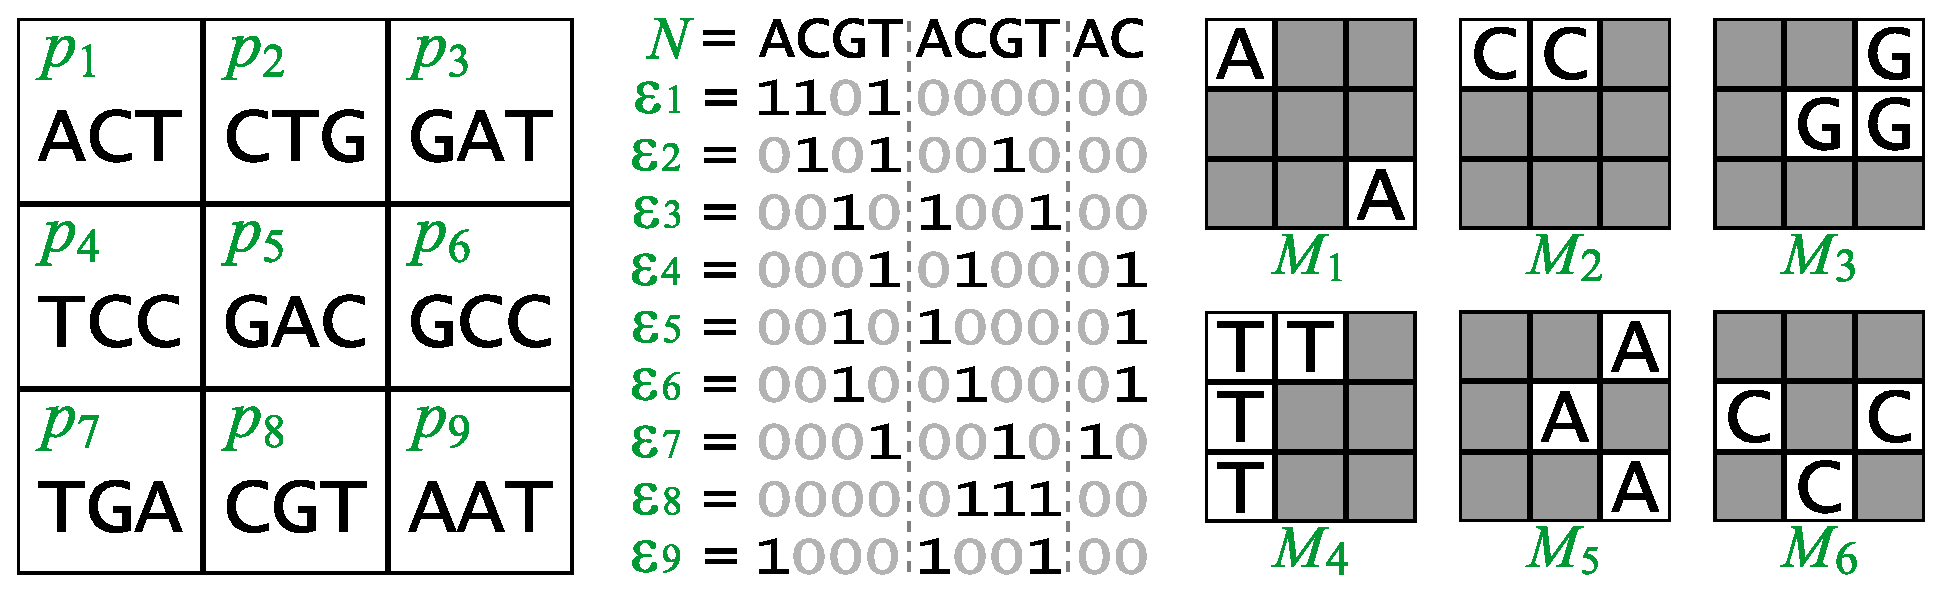
\includegraphics[width=\textwidth]{figures/chip.eps}}
\caption{Synthesis of a hypothetical 3$\times$3 chip with photolithographic
  masks. Left: chip layout and the 3-mer probe sequences. Center: deposition
  sequence with 2.5 cycles (cycles are delimited with dashed lines) and probe
  embeddings (asynchronous). Right: first six masks (masks 7 to 10 not shown).}
\label{fig:masking_process}
\end{figure}

The deposition sequence is often a repeated permutation of the alphabet, mainly
because of its regular structure and because such sequences maximize the number
of distinct subsequences \citep{Chase1976}. The deposition sequence shown in
Figure~\ref{fig:masking_process} is a 2.5-time repetition of \Seq{ACGT}, and we
thus say that it has two and a half \emph{cycles}.

For cyclic deposition sequences, it is possible to distinguish between two types
of embeddings: \emph{synchronous} and \emph{asynchronous}. In the former, each
probe has exactly one nucleotide added in every cycle of the deposition
sequence; hence, 25 cycles or 100 steps are needed to synthesize probes of
length 25. In the latter, probes can have any number of nucleotides added
in any given cycle, allowing shorter deposition sequences. For this reason,
asynchronous embeddings are usually the choice for commercial microarrays.  For
instance, all GeneChip arrays that we know of can be asynchronously synthesized
in 74~steps with $N=(\Seq{TGCA})^{18}\Seq{TG}$., i.e., $18.5$ cycles of
\Seq{TGCA} --- we refer to this sequence as the \emph{standard Affymetrix
deposition sequence} (see Chapter~\ref{ch:affy}).

Ideally, the deposition sequence should be as short as possible in order to
reduce manufacturing time, cost and probability of errors \citep{Rahmann2003}.
Finding the shortest deposition sequence to synthesize a set of probes is an
instance of a classical computer science problem known as the shortest common
supersequence problem, which will be the focus of Chapter~\ref{ch:scs}. For the
MLP, however, we assume that $N$ is a fixed sequence given as input.

%%%%%%%%%%%%%%%%%%%%%%%%%%%%%%%%%%%%%%%%%%%%%%%%%%%%%%%%%%%%%%%%%%%%%%%%%%%%%%%%
\section{Problem statement}
\label{sec:mlp_problem}

Given a set of probes $\CalP$, a geometry of spots $\CalS$, and a deposition
sequence $N$ as specified above, the MLP asks to specify a chip layout
$(\lambda,\eps)$ that consists of
\begin{enumerate}
\item a bijective assignment $\lambda: \CalS\to \{1,\dots,n\}$ that specifies a
  probe index $k(s)$ for each spot $s$ (meaning that $p_{k(s)}$ will be
  synthesized at $s$),
\item an assignment $\eps: \{1,\dots,n\}\to \{0,1\}^T$ specifying an embedding
  $\eps_k = (\eps_{k,1},\dots,\eps_{k,T})$ for each probe index $k$, such that
  $N[\eps_k] :\equiv (N_t)_{t: \eps_{k,t}=1} = p_k$,
\end{enumerate}
such that a given penalty function is minimized.  We introduce two such penalty
functions: total border length and total conflict index.

%We may thus speak of $\eps_{k(s)}$ as the embedding at spot $s$.

%%%%%%%%%%%%%%%%%%%%%%%%%%%%%%%%%%%%%%%%%%%%%%%%%%%%%%%%%%%%%%%%%%%%%%%%%%%%%%%%
\section{Border length}
\label{sec:mlp_border_length}

The first formal definition of the unintended illumination problem was given by
\citet{Hannenhalli2002}, who defined the \emph{border length}~$\CalB_t$ of a
mask~$M_{t}$ as the number of borders separating masked and unmasked spots at
synthesis step~$t$, that is, the number of border conflicts in $M_{t}$.
Formally,
%%
\begin{equation}
\label{eq:border_length}
  \CalB_t := \frac{1}{2} \cdot \sum_{s,s' \in \CalS}
    \Ind{s \text{ and } s' \text{ are adjacent}}
    \cdot \Ind{\eps_{k(s),t} \neq \eps_{k(s'),t}}.
\end{equation}
%%
where $\Ind{cond}$ is the indicator function that equals 1 if condition $cond$
is true, and 0 otherwise. The \emph{total border length} of a given layout
$(\lambda,\eps)$ is the sum of border lengths over all masks, that is
%%
\begin{equation}
\label{eq:total_border_length}
  \CalB(\lambda,\eps) := \sum_{t=1}^{T} \CalB_t.
\end{equation}

The \emph{border length minimization problem} was then defined as the problem of
finding a layout minimizing the total border length \citep{Hannenhalli2002}. As
an example, the six masks shown in Figure~\ref{fig:masking_process} have
$\CalB_1 = 4$, $\CalB_2 = 3$, $\CalB_3 = 5$, $\CalB_4 = 4$, $\CalB_5 = 8$ and
$\CalB_6 = 9$. The total border length of that layout is 52 (masks $M_7$ to
$M_{10}$ are not shown).

\paragraph{Hamming distance.}
In the next chapters, we refer to the \emph{Hamming distance} $H(k,k')$ between
the embeddings $\eps_k$ and $\eps_{k'}$ as the number of synthesis steps in
which they differ. Formally,
%%
\begin{equation}\label{eq:hamming}
  H(k,k') := \sum_{t=1}^{T} \Ind{\eps_{k,t} \neq \eps_{k',t}}.
\end{equation}

Note that $H(k,k')$ gives the number of border conflicts generated when probes
with embeddings $\eps_k$ and $\eps_{k'}$ are placed in adjacent spots.

\subsection{Lower bounds}

Lower bounds for the BLMP with synchronous and asynchronous embeddings were
given by \citet{Kahng2002}, based on a simple graph formulation. Unfortunately,
both lower bounds are not tight, and their computation is time-consuming,
especially for large chips.

\paragraph{Synchronous embeddings.}
Let $L$ be a complete directed graph over the set of probes $\CalP$ with arcs
weighted with the Hamming distance between the (unique) embeddings of the
corresponding probes.

Since a probe can have at most four neighbors on the chip, we delete all but the
four arcs with the least weights of every node. Furthermore, assuming that the
chip is a rectangular grid with $n_r$ rows and $n_c$ columns, we delete the
heaviest $2 \cdot (n_r + n_c)$ remaining arcs, because the spots on the borders
of the chip have less than four neighbors. It is not difficult to see that the
cost of any placement must be greather than the total arc weight of $L$, and we
obtain the following theorem.

\begin{theorem}
  \label{thm:sync_lb}
  The total arc weight of $L$ is a lower bound on the total border length of
  the optimum layout with synchronous embeddings.
\end{theorem}

\paragraph{Asynchronous embeddings.}
With asynchronous embeddings, we can construct a similar complete directed graph
$L'$. For the arc weights, however, it is necessary to estimate the minimum
number of border conflicts between the two probes (among all of their possible
embeddings).

\citet{Kahng2002} observed that the number of bases of a probe $p_k$ that can
be ``aligned'' with bases of $p_{k'}$ cannot exceed the length of $LCS(p_k,p_{k'})$,
where $LCS(p_k,p_{k'})$ is the
\emph{longest common subsequence} of $p_k$ and $p_{k'}$. Therefore, an arc of $L'$
between probes $p_k$ and $p_{k'}$ can be weighted with $\ell - |LCS(p_k,p_{k'})|$,
where $\ell$ is the length of both probe sequences (assuming probes have the same length).

We can then delete all but the four arcs with the least weights of each probe
and, subsequently, the heaviest $2 \cdot (n_r + n_c)$ remaining arcs of $L'$, to
obtain the following theorem.

\begin{theorem}
  \label{thm:async_lb}
  The total arc weight of $L'$ is a lower bound on the total border length of
  the optimum layout with asynchronous embeddings.
\end{theorem}

%%%%%%%%%%%%%%%%%%%%%%%%%%%%%%%%%%%%%%%%%%%%%%%%%%%%%%%%%%%%%%%%%%%%%%%%%%%%%%%%
\section{Conflict index}
\label{sec:mlp_conflict_index}

The border length measures the quality of an individual mask or set of masks.
With this model, however, it is not possible to know how the border conflicts
are distributed among the probes. Ideally, all probes should have roughly the
same risk of being damaged by unintended illumination, so that all signals are
affected in approximately the same way.

The \emph{conflict index} is a quality measure defined with the aim of
estimating the risk of damaging probes at a particular spot
\citep{Carvalho2006a}; it is thus a per-spot or per-probe measure instead of a
per-mask measure. Additionally, it takes into account two practical
considerations observed by \citet{Kahng2003}:
%%
\begin{itemize}
\item[a)] stray light might activate not only adjacent neighbors but also spots
  that lie as far as three cells away from the targeted spot;
\item[b)] imperfections produced in the middle of a probe are more harmful than
  in its extremities.
\end{itemize}

For a proposed layout $(k,\eps)$, the conflict index~$\CalC(s)$ of a spot $s$
whose probe $p_{k(s)}$ is synthesized in $T$~masking steps according to its
embedding vector $\eps_{k(s)}$ is
%%
\begin{equation}
\label{eq:conf_idx}
\CalC(s) := \sum_{t=1}^{T} \Bigl(
  \Ind{\eps_{k(s),t}=0}
  \cdot \omega(\eps_{k(s)},t)
  \cdot \sum_{\substack{s'\text{: neighbor}\\\text{of } s}}
  \Ind{\eps_{k(s'),t}=1}
  \cdot \gamma(s,s') \Bigr).
\end{equation}

The indicator functions ensure the following conflict condition: During
step~$t$, there is a conflict at spot~$s$ if and only if $s$ is masked
($\eps_{k(s),t}=0$) and a close neighbor $s'$ is unmasked ($\eps_{k(s'),t}=1$)
--- since light directed at $s'$ may somehow reach $s$. When $s$ is unmasked, it
does not matter if it accidentally receives light targeted at a neighbor, and
when $s'$ is masked, there is no risk that it damages probes of $s$ since it is
not receiving light.

\begin{figure}[t]\centering
%%
\begin{picture}(435,150)
  \put(0,0){\makebox(180,150){
    \includegraphics[width=0.4\textwidth]{distweights}
  }}
  \put(180,5){\makebox(255,145){
    \includegraphics{posweights}
  }}
\end{picture}
%%
\vspace*{-3ex}
\caption{\label{fig:conflictindex}
  Ranges of values for both $\gamma$ and $\omega$ on a typical Affymetrix chip
  where probes of length $\ell=25$ are synthesized in $T=74$ masking steps.
  Left: approximate values of the distance-dependent weighting function
  $\gamma(s,s')$ for a spot $s$ in the center and close neighbors~$s'$. Right:
  position-dependent weights $\omega(\eps,t)$ on the y-axis for each value of~
  $b_{\eps,t}\in\{0,\dots,25\}$ on the x-axis, using $\theta = 5/\ell$ and
  $c = 1/\exp{(\theta)}$.
  }%
\end{figure}

Function $\gamma(s,s')$ is a ``closeness'' measure between $s$ and $s'$ (to
account for observation a). We define it as
%%
\begin{equation}\label{eq:dist_weight}
\gamma(s,s') := (d(s,s'))^{-2},\nopagebreak
\end{equation}\nopagebreak
%%
where $d(s,s')$ is the Euclidean distance between the spots $s$ and $s'$. Note
that in (\ref{eq:conf_idx}), $s'$ ranges over all neighboring spots that are at
most three cells away from $s$ (see Figure~\ref{fig:conflictindex}, left), which
is in accordance with observation a. In general, we use the terms \emph{close
neighbor} or simply \emph{neighbor} of a spot $s$ to refer to a spot $s'$ that
is at most three cells away (vertically and horizontally) from $s$. In other
words, $s'$ is inside a $7\times 7$ region centered around $s$. This is in
contrast to the terms \emph{direct} or \emph{immediate neighbor} of $s$, used to
denote a spot $s'$ that is adjacent to $s$ (in other words, when $s'$ shares a
common border with $s$ on the chip). Obviously, an immediate neighbor $s'$ is
also a close neighbor of $s$.

The position-dependent weighting function $\omega(\eps,t)$ accounts for the
significance of the location inside the probe where the undesired nucleotide is
introduced in case of accidental illumination (observation b). We defined it as:
%%
\begin{equation}\label{eq:pos_mult}
\omega(\eps,t) := c \cdot \exp{\left(\theta \cdot \lambda(\eps,t)\right)}
\end{equation}
%%
where $c>0$ and $\theta>0$ are constants, and for $1\leq t\leq T$,
%%
\begin{equation}\label{eq:base_pos}
  \lambda(\eps,t) := 1 + \min(b_{\eps,t},\ell_{\eps} - b_{\eps,t}),
\end{equation}
%%
\begin{equation}\label{eq:b_ell}
  b_{\eps,t} := \sum_{t'=1}^{t} \eps_{t'},
  \qquad
  \ell_{\eps} := \sum_{t=1}^{T} \eps_t = b_{\eps,T}.
\end{equation}

In other words, $\ell_\eps$ is the length of the final probe specified by $\eps$
(equal to the number of ones in the embedding), and $b_{\eps,t}$ denotes the
number of nucleotides added up to and including step~$t$. The parameter $\theta$
controls how steeply the exponential weighting function rises towards the middle
of the probe (Figure~\ref{fig:conflictindex}, right). In our experiments, unless
stated otherwise, we use probes of length $\ell=25$, and parameters
$\theta = 5/\ell$ and $c = 1/\exp{(\theta)}$.
We can now speak of the \emph{total conflict index} of a given layout
$(\lambda,\eps)$ as the sum of conflict indices over all spots, that is
%%
\begin{equation}
\label{eq:total_conf_idx}
  \CalC(\lambda,\eps) := \sum_{s} \CalC(s).
\end{equation}

\paragraph{Conflict index distance.}
Many of the algorithms discussed in later chapters were initially developed for
border length minimization, and they usually rely on the Hamming distance
defined earlier (\ref{eq:hamming}). We have adapted some of these algorithms to
work with conflict index minimization by using the \emph{conflict index
distance}, which extends the Hamming distance by taking into account the
position inside the probe where the conflict occurs (observation b). The
conflict index distance $C(k,k')$ between the embeddings $\eps_k$ and
$\eps_{k'}$ is defined as:
%%
\begin{equation}
\label{eq:ci_dist}
C(k,k') := \sum_{t=1}^{T}
  \Bigl(
    \Ind{\eps_{k,t}=0 \text{ and } \eps_{k',t}=1}
    \cdot \omega(\eps_{k},t)
    +
    \Ind{\eps_{k',t}=0 \text{ and } \eps_{k,t}=1}
    \cdot \omega(\eps_{k'},t)
  \Bigr).
\end{equation}

The conflict index distance $C(k,k')$ can be interpreted as the sum of the
conflict indices resulting from placing probes with embeddings $\eps_k$ and
$\eps_{k'}$ at hypothetical neighboring spots, ignoring the distance between
these spots (note that there is no dependency on $\gamma$) and the conflicts
generated by other neighbors.

\subsection{The choices of $\gamma$ and $\omega$}

The conflict index $\CalC(s)$ attempts to estimate the risk of damaging the
probes of a spot $s$ due to unintended illumination. The definitions of $\gamma$
and $\omega$ given here are an arbitrary choice in an attempt to capture the
characteristics of the problem.

However, the most appropriate choice of $\gamma$ depend on several attributes of
the specific technology utilized to produce the chips such as the size of the
spots, the density of the probes on the chip, the physical properties of the
light being used (intensity, frequency, etc.), the distance between the light
source and the mask, and the distance between the mask (or the micromirrors) and
the chip surface.

The most appropriate choice of $\omega$ depend on the chemical properties of the
hybridization between probes and targets. Although it is generally agreed that
the chances of a successful hybridization are higher if a mismatched base occurs
at the extremities of the formed duplex instead of at its center
\citep{Hubbell1999,Southern1999,Guo1997}, the precise effects of this position
is not yet fully understood and has been an active topic of research
\citep{Binder2004,Binder2005}.

We propose the use of an exponential function, so that $\omega$ grows
exponentially from the extremities of the probe to its center (see
Figure~\ref{fig:conflictindex}, right). The motivation behind this definition is
that the probability of a successful stable hybridization of a probe with its
target should increase exponentially with the absolute value of its Gibbs free
energy, which increases linearly with the length of the longest perfect match
between probe and target.

Finding the best choice of $\gamma$ and $\omega$ for a particular technology is
beyond the scope of this thesis. We note, however, that all algorithms discussed
in the next chapters were developed to work independently of the values given by
these functions. In other words, should $\gamma$ and $\omega$ be defined
differently, no changes to the algorithms are necessary.

%%%%%%%%%%%%%%%%%%%%%%%%%%%%%%%%%%%%%%%%%%%%%%%%%%%%%%%%%%%%%%%%%%%%%%%%%%%%%%%%
\section{Chip quality measures}
\label{sec:mlp_bl_vs_ci}

Most of the algorithms discussed in the next chapters can work with border
length as well as conflict index minimization. In our experiments, we will
usually present results with both measures, making a distinction between border
length minimization (BLM) and conflict index minimization (CIM).

The relation between these two
measures becomes clear if $\gamma(s,s')$ and $\omega(\eps,t)$ are re-defined as
follows: Set $\gamma(s,s') := 1$ if $s'$ is a direct neighbor of~ $s$, and $:=0$
otherwise. Also, set $c=1/2$ and $\theta=0$ so that $\omega(\eps,t) := 1/2$
independently of the position in the probe where the conflict occurs. Now
$\sum_s\, \CalC(s) = \sum_{t=1}^T\, \CalB_t$; that is, total border length is
equivalent to the total conflict index for a particular choice of $\gamma$ and
$\omega$. For the choices~(\ref{eq:dist_weight}) and~(\ref{eq:pos_mult}), they
are not equivalent but still correlated, since a good layout has low border
lengths as well as low conflict indices.

To better compare border lengths for chips of different sizes, we usually divide
the total border length by the number $n_b$ of internal borders of the chip,
which equals $n_r(n_c - 1) + n_c(n_r - 1)$ if the the chip is a rectangular grid
with $n_r$ rows and $n_c$ columns. We thus call $\CalB(\lambda,\eps)/n_b$ the
\emph{normalized border length}, NBL for short, of a given layout
$(\lambda,\eps)$. This can be further divided by the number of synthesis steps
to give the \emph{normalized border length per mask}
$\CalB(\lambda,\eps)/(n_b \cdot T)$. We may also refer to the normalized border
length of a particular mask $M_t$ as $B_t/n_b$. Since $B_t \leq n_b$,
$B_t/n_b \leq 1$ and thus $\CalB(\lambda,\eps)/n_b \leq T$.

Similarly, it is useful to divide the total conflict index by the number of
probes on the chip, and we define the \emph{average conflict index}, ACI for
short, of a layout as $\CalC(\lambda,\eps)/|\CalP|$.

%%%%%%%%%%%%%%%%%%%%%%%%%%%%%%%%%%%%%%%%%%%%%%%%%%%%%%%%%%%%%%%%%%%%%%%%%%%%%%%%
\section{How hard is the microarray layout problem?}
\label{sec:mlp_how_hard}

The MLP appears to be hard because of the super-exponential number of possible
arrangements, although no NP-hardness proof is yet known. A formulation of the
MLP as a quadratic assignment problem (QAP) is given in Chapter~\ref{ch:qap}.
The QAP is a classical combinatorial optimization problem that is, in general,
NP-hard, and particularly hard to solve in practice \citep{Cela1997}. Optimal
solutions are thus unlikely to be found even for small chips and even if we
assume that all probes have a single predefined embedding.

If we consider all possible embeddings (up to several million for a typical
Affymetrix probe), the MLP is even harder. For this reason, the problem has been
traditionally tackled in two phases. First, an initial embedding of the probes
is fixed and an arrangement of these embeddings on the chip with minimum
conflicts is sought. This is usually referred to as the \emph{placement} phase.
Second, a post-placement optimization phase \emph{re-embeds} the probes
considering their location on the chip, in such a way that the conflicts with
neighboring spots are further reduced. Often, the chip is \emph{partitioned}
into smaller sub-regions before the placement phase in order to reduce running
times, especially on larger chips.

The most important placement algorithms are surveyed in
Chapter~\ref{ch:placement}, whereas re-embedding algorithms are discussed in
Chapter~\ref{ch:reembed}. Partitioning algorithms are the focus of
Chapter~\ref{ch:part}. Finally, we present recent developments that
simultaneously place and re-embed probes in Chapter~\ref{ch:merge}.

%%%%%%%%%%%%%%%%%%%%%%%%%%%%%%%%%%%%%%%%%%%%%%%%%%%%%%%%%%%%%%%%%%%%%%%%%%%%%%%%
\chapter{Placement Algorithms}
\label{ch:placement}
%%%%%%%%%%%%%%%%%%%%%%%%%%%%%%%%%%%%%%%%%%%%%%%%%%%%%%%%%%%%%%%%%%%%%%%%%%%%%%%%

The input for a placement algorithm consists of a geometry of spots
$\mathcal{S}$, the deposition sequence $N$, and a set of probes $\mathcal{P}$,
where each probe is assumed to have at least one embedding in $N$. The output is
a one-to-one assignment $\lambda$ of probes to spots. If there are more spots
than probes to place, one can add enough ``empty'' probes that do not introduce
any conflicts with the other probes (since light is never directed to their
spots).

All algorithms discussed in this section assume that an initial embedding of the
probes is given, which can be a left-most, right-most, synchronous or otherwise
pre-computed embedding --- a placement algorithm typically does not change the
given embeddings.

%%%%%%%%%%%%%%%%%%%%%%%%%%%%%%%%%%%%%%%%%%%%%%%%%%%%%%%%%%%%%%%%%%%%%%%%%%%%%%%%
\section{Optimal masks for uniform arrays}
\label{sec:placement_uniform}

\citet{Feldman1994} were the first to formally address the unintended
illumination problem. They showed how a placement for a \emph{uniform array}
with minimum number of border conflicts can be constructed using a
two-dimensional Gray code. Uniform arrays are arrays containing all $4^\ell$
probes of a given length $\ell$, which require a deposition sequence of length
$4\cdot \ell$. These arrays were initially developed for the technique known as
Sequencing by Hybridization \citep{Southern1992}.

\begin{figure}[t]\centering
\includegraphics[width=\textwidth]{place/uniform_placement}
\caption{\label{fig:uniform_placement}%
  Construction of a placement for uniform arrays (containing the complete set of
  $\ell$-mer probes) based on a two-dimensional Gray code, resulting in layouts
  with minimum number of border conflicts.}
\end{figure}

In general, the term Gray code refers to an ordering of a set of elements in
which successive elements differ in some pre-specified, usually small, way
\citep{Savage1997}. The construction of Feldman and Pevzner is based on a
two-dimensional Gray code composed of strings of length $\ell$ over a
four-letter alphabet. It generates a $2^\ell \times 2^\ell$ array filled with
$\ell$-mer probes in which each pair of adjacent probes (horizontally or
vertically) differs by exactly one letter. This construction is illustrated in
Figure~\ref{fig:uniform_placement}. An $(\ell + 1)$-mer array is constructed by
first copying the $\ell$-mer array into the upper left quadrant of the
$(\ell + 1)$-mer array and reflecting it horizontally and vertically into the
other three quadrants. The letter in front of the probes in the upper left
quadrant of the $\ell$-mer array is added to all probes in the upper left
quadrant of the $(\ell + 1)$-mer array. The probes of the other three quadrants
are extended in the same way.

It can be shown that such placement generates masks with a minimum number of
border conflicts if probes are synchronously embedded (see
Figure~\ref{fig:uniform_masks}). However, because this construction is
restricted to uniform arrays and synchronous embeddings, it is of limited
practical importance for current microarrays.

\begin{figure}[t]\centering
\begin{picture}(435,175)
\put(0,0){ \makebox(435,175){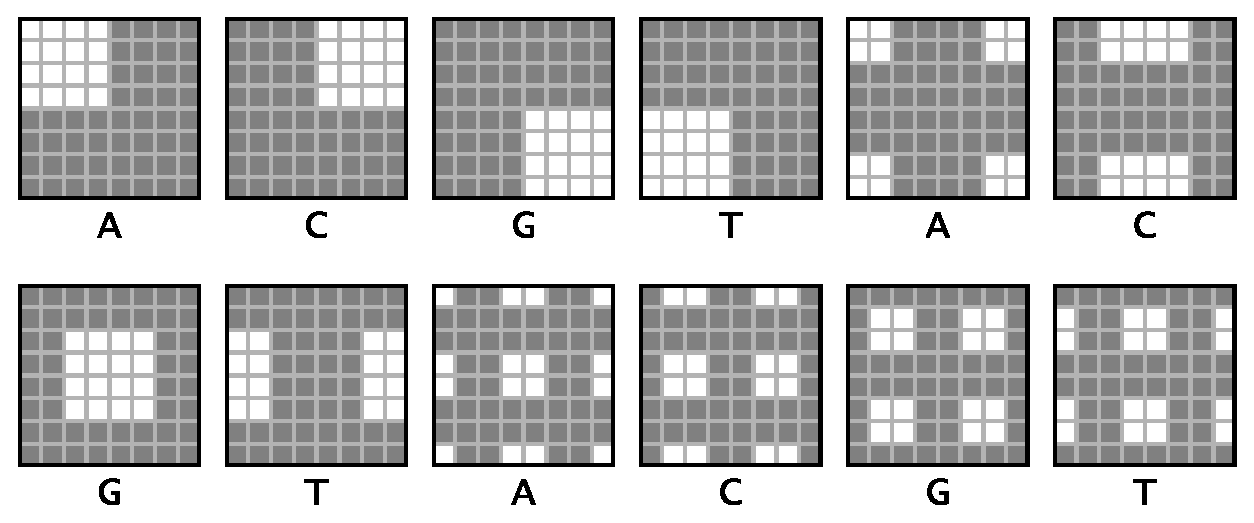
\includegraphics[width=\textwidth]{place/uniform_masks}}}
\end{picture}
\caption{\label{fig:uniform_masks}%
  Masks for the $8\times 8$ uniform array of Figure~\ref{fig:uniform_placement}
  when probes are synchronously embedded into $(\Seq{ACGT})^{3}$. Masked spots
  are represented by shaded squares, unmasked spots by white squares. Note that
  masks of the same cycle have the same number of border conflicts.}
\end{figure}

%%%%%%%%%%%%%%%%%%%%%%%%%%%%%%%%%%%%%%%%%%%%%%%%%%%%%%%%%%%%%%%%%%%%%%%%%%%%%%%%
\section{TSP and threading algorithms}
\label{sec:placement_threading}

The border length problem on arrays of arbitrary probes was first discussed by
\citet{Hannenhalli2002}. The article reports that the first Affymetrix chips
were designed using a heuristic for the traveling salesman problem (TSP). The
idea is to build a weighted graph with nodes representing probes, and edges
containing the Hamming distances between their embeddings (see Equation
\ref{eq:hamming}). A TSP tour on this graph is heuristically constructed and
\emph{threaded} on the array in a row-by-row fashion
(Figure~\ref{fig:threading}a).

For uniform arrays, every solution of the TSP corresponds to a (one-dimensional)
Gray code since consecutive elements in the tour differ in only one position,
thus minimizing border conflicts between neighboring probes. For general arrays,
a TSP solution also reduces border conflicts as consecutive probes in the tour
are likely to be similar. Threading the (one-dimensional) tour on a
two-dimensional chip, row-by-row, on a leads to an arrangement where consecutive
probes in the same row have few border conflicts, but probes in the same column
may have very different embeddings.

Another problem of this approach is that the TSP is known to be NP-hard
\citep{Gross2004}, so computing an optimal TSP tour even for a small
$300\times 300$ array is not feasible, and only fast approximation algorithms
are suitable. In practice, Hannenhalli et.~al.\ managed to achieve
marginal improvements in tour cost using the 2-opt algorithm for TSP of
\citet{Lin1973} and an algorithm for weighted matching due to \citet{Gabow1976}.
Unfortunately, their efforts resulted in only $1.05\%$ reduction in tour cost
for a chip with $66\,000$ probes when compared to the greedy TSP algorithm
initially used at Affymetrix.

\begin{figure}[t]\centering
\begin{picture}(435,130)
\put(-2,0){ \makebox(145,15){a)}}
\put(147,0){\makebox(145,15){b)}}
\put(292,0){\makebox(145,15){c)}}
\put(-2,15){ \makebox(145,115){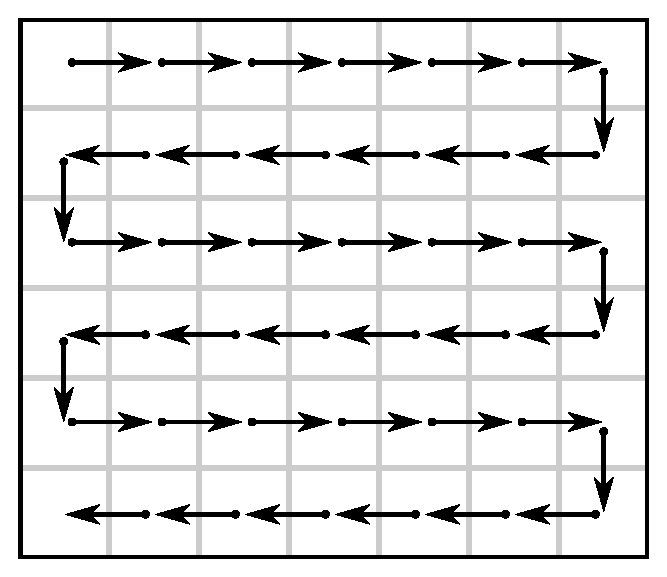
\includegraphics[width=0.3\textwidth]{0threading}}}
\put(147,15){\makebox(145,115){\includegraphics[width=0.3\textwidth]{1threading}}}
\put(292,15){\makebox(145,115){\includegraphics[width=0.3\textwidth]{2threading}}}
\end{picture}
\caption{\label{fig:threading}%
  Different ways of \emph{threading} probes on a chip. a) Standard row-by-row
  (0-threading); b) 1-threading; c) 2-threading.}
\end{figure}

Since improvements in the cost of the TSP tour seemed unlikely, Hannenhalli
et.~al.\ turned their attention to the problem of threading the tour on the
chip. They studied several threading alternatives, which they collectively
called \emph{$k$-threading} (Figure~\ref{fig:threading}). A $k$-threading is a
variation of the standard row-by-row threading, in which the right-to-left and
left-to-right paths are interspaced with alternating upward and downward
movements over $k$ sites (the row-by-row threading can be seen as a
$k$-threading with $k=0$); $k$ is called the \emph{amplitude} of the threading.
Hannenhalli et.~al.\ experimentally observed that 1-threading may reduce total
border length of layouts constructed with TSP tours in up to 20\% for large
chips when compared to row-by-row threading.

From now on, we will use the term TSP\,+$k$-threading to refer to the method of
computing a TSP tour and threading it on the array using $k$-threading.

%%%%%%%%%%%%%%%%%%%%%%%%%%%%%%%%%%%%%%%%%%%%%%%%%%%%%%%%%%%%%%%%%%%%%%%%%%%%%%%%
\section{Epitaxial placement}
\label{sec:placement_epitaxial}

A different strategy inspired by techniques used in the design of VLSI circuits,
called Epitaxial placement, or \emph{seeded crystal growth}, was proposed by
\citet{Kahng2002}. It essentially grows a placement around a single starting
``seed'' using a greedy heuristic. Although it was originally designed for chips
with synchronous embeddings, it can be trivially implemented for asynchronous
embeddings as well.

The algorithm starts by placing a random probe in the center of the array and
continues to insert probes in spots adjacent to already-filled spots. Priority
is given to spots whose all four neighbors are filled, in which case a probe
with the minimum number of border conflicts with the neighbors is placed.
Otherwise, all spots with $1 \leq i < 4$ filled neighbors are examined. For each
spot $s$, the algorithm finds a non-assigned probe~$p$ whose number of border
conflicts with the filled neighbors of $s$, $c(s,p)$, is minimal and assigns a
normalized cost $\bar{c}(s,p) := \sigma_i \cdot c(s,p) / i$ for this assignment,
where $0 < \sigma_i \leq 1$ are scaling coefficients (the authors propose
$\sigma_1 = 1$, $\sigma_2 = 0.8$, and $\sigma_3 = 0.6$). The assignment with
minimum $\bar{c}(s,p)$ is made and the procedure is repeated until all probes
have been placed.

In order to avoid repeated cost computations, the authors propose keeping a list
of probe candidates, for each spot, sorted by their normalized costs. This list
must be updated whenever one of its neighbors is filled; thus, it is updated at
most four times (but only two times on average).

With this algorithm, Kahng et.~al.\ claim a further 10\% reduction in
border conflicts over the TSP\,+\,1-threading approach of
\citet{Hannenhalli2002}. However, the Epitaxial algorithm has
at least quadratic time complexity as it examines every non-placed probe to fill
each spot, and large memory requirements if a list of probe candidates is kept
for each spot. Hence, like the TSP approach, it does not scale well to large
chips. In their experiments, the Epitaxial algorithm needed 274 seconds to
design a $100\times 100$ chip, but $4\,441$ seconds to design a $200\times 200$
chip. That is a $16.2$-fold increase in running time for a 4-fold increase in
number of spots. Chips of larger dimensions could not be computed because of
prohibitively large running time and memory requirements.

%%%%%%%%%%%%%%%%%%%%%%%%%%%%%%%%%%%%%%%%%%%%%%%%%%%%%%%%%%%%%%%%%%%%%%%%%%%%%%%%
\section{Sliding-Window Matching}
\label{sec:placement_swm}

\begin{figure}[t!]\centering
\centerline{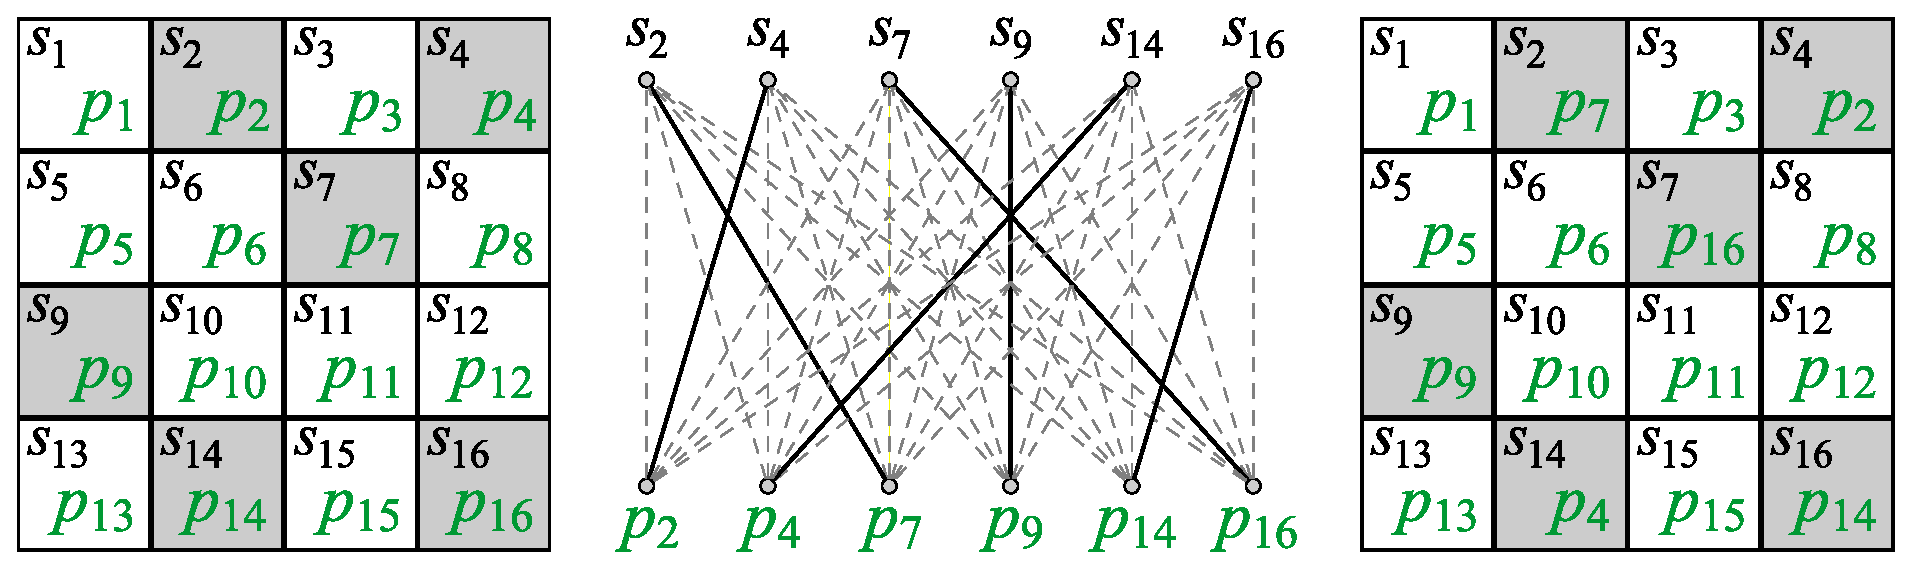
\includegraphics[width=\textwidth]{swm.eps}}
\begin{picture}(435,20)
\put(-3,0){ \makebox(125,20){a)}}
\put(139,0){\makebox(159,20){b)}}
\put(313,0){\makebox(125,20){c)}}
\end{picture}
\caption{\label{fig:swm}%
  Sliding-Window Matching algorithm. a) Initial arrangement of probes
  $p_1$ to $p_{16}$ inside a $4 \times 4$ window (with spots $s_1$ to $s_{16}$
  and a selected maximal independent set of spots (shaded). b) Bipartite graph
  with selected probes and spots, and a minimum weight perfect matching (dark
  edges) resulting in a minimum cost re-assignment of probes to spots. c) New
  arrangement inside the window according to the perfect matching.}%
\end{figure}

The Sliding-Window Matching algorithm \citep{Kahng2003}, SWM for short, is not
exactly a placement algorithm as it iteratively improves an existing placement
that can be constructed, for instance, by TSP\,+\,1-threading (Section
\ref{sec:placement_threading}).

The authors noted that the TSP tour can be conveniently substituted by
lexicographically sorting the probe sequences or, alternatively, their binary
embedding vectors with a linear-time radix sort. The sorting is faster, but it
is also likely to produce a worse initial placement than the TSP tour, with
consecutive embeddings being similar only in their first synthesis steps. The
authors argue that this is of little importance in practice given that this
placement is only used as a starting point for the SWM algorithm, and the
lexicographical sorting should be the choice for large microarrays because
computing a TSP tour takes prohibitively long for chips larger than
$500\times 500$ spots. (From now on, we will use the term
sorting\,+$k$-threading, or simply $k$-threading, to refer to the method of
sorting probes lexicographically and threading them on the array using
$k$-threading.)

As its name implies, SWM works inside a window that starts at the top left of
the chip and slides from left to right, top to bottom, while maintaining a
certain amount of overlap between each iteration. When the window reaches the
right-end of the chip, it is re-started at the left-end of the next set of rows,
also retaining an overlap with the preceding set of rows.

At each iteration, the algorithm attempts to reduce the total border length
inside the window by relocating some of its probes (Figure~\ref{fig:swm}a).
First, a random maximal independent set of spots is selected, and the probes
assigned to these spots are removed. The term independent refers to the fact
that selected spots can be re-assigned to probes without affecting the border
length of other selected spots. The algorithm then creates a bipartite graph
with nodes representing the removed probes and the now vacant spots
(Figure~\ref{fig:swm}b). The edges of this graph are weighted with the number of
border conflicts that are generated by the corresponding assignment.  Finally, a
minimum weight perfect matching on this graph is computed, and the indicated
assignments are made (Figure~\ref{fig:swm}c).

A minimum weight perfect matching requires polynomial time \citep{Gross2004},
but the small graphs generated by SWM can be computed rather quickly. The
authors experimentally observed that the best results are obtained with small
window sizes (e.g. $6\times 6$) and an overlap of half the window size.
Moreover, employing less effort in each window and executing more cycles of
optimization gives better results than more effort in each window and less
cycles.

Selecting an independent set of spots ensures that the cost of each new
assignment can be computed independently of the other assignments. The SWM was
designed for border length minimization (BLM) and it takes advantage of the fact
that, in this model, an independent set of spots can be constructed by selecting
spots that do not share a common border. SWM can be adapted for conflict index
minimization (CIM) by using larger windows containing relatively sparse
independent sets (to our knowledge, this has not been implemented yet).
Therefore several random independent sets should be constructed before moving
the window.

%%%%%%%%%%%%%%%%%%%%%%%%%%%%%%%%%%%%%%%%%%%%%%%%%%%%%%%%%%%%%%%%%%%%%%%%%%%%%%%%
\section{Row-Epitaxial}
\label{sec:placement_reptx}

Row-Epitaxial \citep{Kahng2003} is a variant of the Epitaxial algorithm with two
main differences introduced to improve scalability: i) spots are filled in a
pre-defined order, namely, from top to bottom, left to right, and ii) only a
limited number $Q$ of probe candidates are considered for filling each spot.

Like SWM, Row-Epitaxial improves an initial placement that can be constructed
by, for example, sorting\,+\,1-threading. For each spot $s$ with a probe $p$,
it looks at the next $Q$ probes that lie in close proximity (to the right or
below $s$), and swaps $p$ with the probe that generates the minimum number of
border conflicts between $s$ and its left and top neighbors.

In the experiments conducted by \citet{Kahng2003,Kahng2004}, Row-Epitaxial was
the best large-scale placement algorithm (for BLM), achieving up to 9\%
reduction in border conflicts over TSP\,+\,1-threading, whereas SWM achieved
slightly worse results but required significantly less time.

Row-Epitaxial can also be adapted to CIM by swapping a probe of a spot $s$ with
the probe candidate that minimizes the sum of conflict indices in a region
around $s$ restricted to those neighboring probes that are to the left or above
$s$ (those which have already found their final positions).

Table~\ref{tab:reptx} shows the results of using Row-Epitaxial for both border
length and conflict index minimization on chips with random probe sequences
(uniformly generated). Probes were lexicographically sorted and left-most
embedded into the standard 74-step Affymetrix deposition sequence and threaded
on the array with $k$-threading. The resulting layouts were then used as a
starting point for Row-Epitaxial.

Although \citet{Hannenhalli2002} suggested 1-threading for laying out a TSP tour
on the chip, our results show that increasing the threading's amplitude from
$k=0$ to $k=4$ usually improves the initial layout produced by
sorting\,+\,$k$-threading, both in terms of border length and conflict index
minimization. For example, increasing the amplitude from $k=0$ to $k=4$ reduced
the normalized border length of the initial layout in up to $6.56\%$ (from
$23.6828$ to $22.1279$) and the average conflict index in up to $4.51\%$ (from
$689.6109$ to $658.5097$) on $800\times 800$ chips.

However, the best initial layouts rarely led to the best final layout produced
by Row-Epitaxial. With BLM the best results were usually achieved with $k=0$,
whereas with CIM there was no clear best value for $k$. In any case, the
difference due to varying $k$ for the threading were rather small for
Row-Epitaxial --- at most $0.78\%$ in normalized border length (from $16.9760$
with $k=0$ to $17.1085$ with $k=4$) and $0.26\%$ in average conflict index (from
$448.0140$ with $k=0$ to $449.1653$ with $k=4$), both on a $800\times 800$ chip
with $Q=5$K (we use ``K'' to denote a multiple of a thousand).

\begin{table}[p!]\centering
\caption{\label{tab:reptx}
  Normalized border length and average conflict index of layouts produced by
  Row-Epitaxial (Row-Eptx) on random chips of various dimensions, with initial
  layouts produced by sorting\,+\,$k$-threading. Running times are reported
  in minutes and include the time for $k$-threading and Row-Epitaxial. All
  results are averages over a set of five chips.}
\footnotesize{
\begin{tabular*}{\hsize}{crrlrrrlrrr}
\vspace{1pt}
     &     &     & & \multicolumn{3}{c}{Border length minimization} & & \multicolumn{3}{c}{Conflict index minimization} \\ \cline{5-7} \cline{9-11}
\vspace{1pt}
Dim. & $Q$ & $k$ & & $k$-threading & Row-Eptx & Time                & & $k$-threading & Row-Eptx & Time \\
\hline
$300\times 300$ &  5K & 0 &   &      24.9649  & {\bf 18.2935} &  1.1 &  &      701.8698  &      462.5194  &   4.9 \\
                &     & 1 &   &      24.1235  &      18.2999  &  1.3 &  &      690.8091  & {\bf 462.4656} &   5.1 \\
                &     & 2 &   &      23.8695  &      18.3072  &  1.2 &  &      685.5916  &      462.6394  &   4.6 \\
                &     & 3 &   &      23.7993  &      18.3226  &  1.2 &  &      683.5980  &      462.5885  &   5.1 \\
                &     & 4 &   & {\bf 23.7588} &      18.3279  &  1.3 &  & {\bf 682.3542} &      462.7775  &   5.1 \\
\cline{2-11}
                & 10K & 0 &   &      24.9649  & {\bf 18.1477} &  2.8 &  &      701.8698  &      444.0354  &   9.7 \\
                &     & 1 &   &      24.1235  &      18.1529  &  2.8 &  &      690.8091  &      444.0904  &   9.3 \\
                &     & 2 &   &      23.8695  &      18.1519  &  2.9 &  &      685.5916  &      444.1960  &  10.0 \\
                &     & 3 &   &      23.7993  &      18.1591  &  2.8 &  &      683.5980  & {\bf 443.9850} &  10.6 \\
                &     & 4 &   & {\bf 23.7588} &      18.1603  &  2.9 &  & {\bf 682.3542} &      444.1745  &   9.8 \\
\cline{2-11}
                & 20K & 0 &   &      24.9649  &      18.0274  &  7.2 &  &      701.8698  &      426.7824  &  18.9 \\
                &     & 1 &   &      24.1235  &      18.0325  &  6.9 &  &      690.8091  &      426.8863  &  18.5 \\
                &     & 2 &   &      23.8695  &      18.0277  &  6.6 &  &      685.5916  &      426.8832  &  19.3 \\
                &     & 3 &   &      23.7993  & {\bf 18.0272} &  6.6 &  &      683.5980  &      426.8694  &  19.6 \\
                &     & 4 &   & {\bf 23.7588} &      18.0321  &  7.5 &  & {\bf 682.3542} & {\bf 426.6600} &  20.2 \\
\hline
$500\times 500$ &  5K & 0 &   &      24.2693  & {\bf 17.6000} &  4.3 &  &      693.5428  &      456.2042  &  15.2 \\
                &     & 1 &   &      23.3454  &      17.6095  &  4.1 &  &      682.2097  & {\bf 456.1341} &  15.2 \\
                &     & 2 &   &      23.0797  &      17.6246  &  4.3 &  &      676.4884  &      456.5261  &  14.1 \\
                &     & 3 &   &      22.9632  &      17.6474  &  3.8 &  &      672.8160  &      456.5337  &  14.1 \\
                &     & 4 &   & {\bf 22.9162} &      17.6670  &  3.7 &  & {\bf 671.2636} &      456.8203  &  15.3 \\
\cline{2-11}
                & 10K & 0 &   &      24.2693  & {\bf 17.4503} & 13.1 &  &      693.5428  &      438.7075  &  33.9 \\
                &     & 1 &   &      23.3454  &      17.4523  & 12.8 &  &      682.2097  &      438.7379  &  33.6 \\
                &     & 2 &   &      23.0797  &      17.4582  & 12.7 &  &      676.4884  & {\bf 438.6477} &  30.4 \\
                &     & 3 &   &      22.9632  &      17.4685  & 12.5 &  &      672.8160  &      438.8183  &  30.8 \\
                &     & 4 &   & {\bf 22.9162} &      17.4755  & 12.5 &  & {\bf 671.2636} &      438.9280  &  32.8 \\
\cline{2-11}
                & 20K & 0 &   &      24.2693  &      17.3303  & 28.2 &  &      693.5428  &      421.1358  &  66.7 \\
                &     & 1 &   &      23.3454  & {\bf 17.3297} & 29.0 &  &      682.2097  &      421.1580  &  63.6 \\
                &     & 2 &   &      23.0797  &      17.3308  & 27.4 &  &      676.4884  &      421.1087  &  67.7 \\
                &     & 3 &   &      22.9632  &      17.3344  & 27.4 &  &      672.8160  & {\bf 420.9758} &  65.1 \\
                &     & 4 &   & {\bf 22.9162} &      17.3376  & 27.7 &  & {\bf 671.2636} &      421.0436  &  64.2 \\
\hline
$800\times 800$ &  5K & 0 &   &      23.6818  & {\bf 16.9760} & 12.2 &  &      689.6109  & {\bf 448.0140} &  36.9 \\
                &     & 1 &   &      22.6092  &      16.9927  & 12.2 &  &      672.2254  &      448.1474  &  40.3 \\
                &     & 2 &   &      22.3205  &      17.0187  & 11.7 &  &      664.9753  &      448.6130  &  38.6 \\
                &     & 3 &   &      22.1958  &      17.0589  & 11.7 &  &      660.5923  &      448.9159  &  40.2 \\
                &     & 4 &   & {\bf 22.1279} &      17.1085  & 12.0 &  & {\bf 658.5097} &      449.1653  &  40.0 \\
\cline{2-11}
                & 10K & 0 &   &      23.6818  & {\bf 16.8032} & 37.0 &  &      689.6109  & {\bf 432.2283} &  88.2 \\
                &     & 1 &   &      22.6092  &      16.8111  & 39.1 &  &      672.2254  &      432.5153  &  91.4 \\
                &     & 2 &   &      22.3205  &      16.8235  & 37.7 &  &      664.9753  &      432.5031  &  85.8 \\
                &     & 3 &   &      22.1958  &      16.8353  & 37.7 &  &      660.5923  &      432.6652  &  90.1 \\
                &     & 4 &   & {\bf 22.1279} &      16.8622  & 39.0 &  & {\bf 658.5097} &      432.6980  &  91.9 \\
\cline{2-11}
                & 20K & 0 &   &      23.6818  & {\bf 16.6771} & 83.1 &  &      689.6109  & {\bf 415.6470} & 174.2 \\
                &     & 1 &   &      22.6092  &      16.6803  & 83.2 &  &      672.2254  &      415.7402  & 181.1 \\
                &     & 2 &   &      22.3205  &      16.6851  & 83.4 &  &      664.9753  &      415.6622  & 179.7 \\
                &     & 3 &   &      22.1958  &      16.6915  & 86.5 &  &      660.5923  &      415.7609  & 172.3 \\
                &     & 4 &   & {\bf 22.1279} &      16.7007  & 80.3 &  & {\bf 658.5097} &      415.7951  & 190.9 \\
\hline
\end{tabular*}}
\end{table}

Our results also give further indication that the running time of Row-Epitaxial
is approximately $O(Qn)$, i.e., linear in the chip size, where $Q$ is a
user-defined parameter that controls the number of probe candidades examined for
each spot. In this way, solution quality can be traded for running time: More
candidates yield better layouts but also demand more time.

%%%%%%%%%%%%%%%%%%%%%%%%%%%%%%%%%%%%%%%%%%%%%%%%%%%%%%%%%%%%%%%%%%%%%%%%%%%%%%%%
\section{Greedy}
\label{sec:placement_greedy}

As discussed in the previous section, the best results obtained with
Row-Epitaxial rarely came from the best initial layouts (produced by
$k$-threading). This is probably because Row-Epitaxial ignores the probe order
used by $k$-threading when it looks for probe candidates to fill a certain spot
(Row-Epitaxial always looks for candidates in the next $Q$ spots, row-by-row,
regardless of how probes were threaded on the array). Another possible
disadvantage of the $k$-threading\,+\,Row-Epitaxial approach is that each swap
made by Row-Epitaxial shuffles the probes in the not-changed spots, destroying
the lexicographical order used during the threading.

In this section, we present a new placement algorithm, Greedy, that combines the
Row-Epitaxial greedy heuristic and a $k$-threading filling strategy in a single
phase, using a linked list of probes to maintain the probe order during the
whole placement. Like Row-Epitaxial, Greedy fills the spots in a greedy fashion,
i.e., for each spot $s$, it examines $Q$ probe candidates and chooses the one
that can be placed at $s$ with minimum cost (Greedy can also be easily
implemented for border length as well as for conflict index minimization).

There are two main differences to Row-Epitaxial. First, instead of (re-)filling
spots row-by-row, spots are filled with $k$-threading (there is no need for an
initial layout). Perhaps more importantly, Greedy sorts the probes
lexicographically and keeps them in a doubly-linked list. This list is used to
maintain the lexicographical order during placement. Moreover, it is also used
to improve the chances of finding a candidate having fewer conflicts with the
last placed probe (which will be its neighbor on the chip): Once a probe $p$ is
selected to fill a certain spot, it is removed from the list and the next search
of candidates examines the probes around $p$'s former position in the list,
e.g., $Q/2$ probes to the left and to the right of $p$.

Table~\ref{tab:greedy} shows the results of using Greedy for both border length
and conflict index minimization on the same set of (random) chips that have been
previously used for the experiments with Row-Epitaxial
(Table~\ref{tab:reptx}). The best layouts were always achieved with $k=0$.
Interestingly, increasing the amplitude of the threading from $k=1$ to $k=4$
always improved the results in terms of border length. In terms of conflict
index, increasing $k$ from 1 to 3 worsened the results; in most cases,
increasing it from 3 to 4 improved the results.

In terms of BLM, Greedy and Row-Epitaxial produced similar results, with the
best layout of Greedy being sometimes marginally better and sometimes marginally
worse than the best layout of Row-Epitaxial. In terms of CIM, however, Greedy
was constantly and significantly better than Row-Epitaxial, achieving up to
$5.65\%$ reduction in average conflic index (from $415.6470$ to $392.1786$) on a
$800\times 800$ chip with $Q=20$K.

In our results, Greedy was between $13.9\%$ and $59.9\%$ slower than
Row-epitaxial in the BLM case ($19.7\%$ on average), and between $3.7\%$
and $18.1\%$ in the CIM case (only $5.6\%$ on average). The difference between
Row-epitaxial and Greedy drops in the CIM case because the extra time spent in
computing the cost of each candidate is higher than in the BLM case, which
reduces the impact of the time required to keep the doubly-linked list.

\begin{figure}\centering
%%
\begin{picture}(438,200)\footnotesize{
  \put(0,0){\makebox(215,200){
    \includegraphics{place/tradeoff/bl}
  }}
  \put(223,0){\makebox(215,200){
    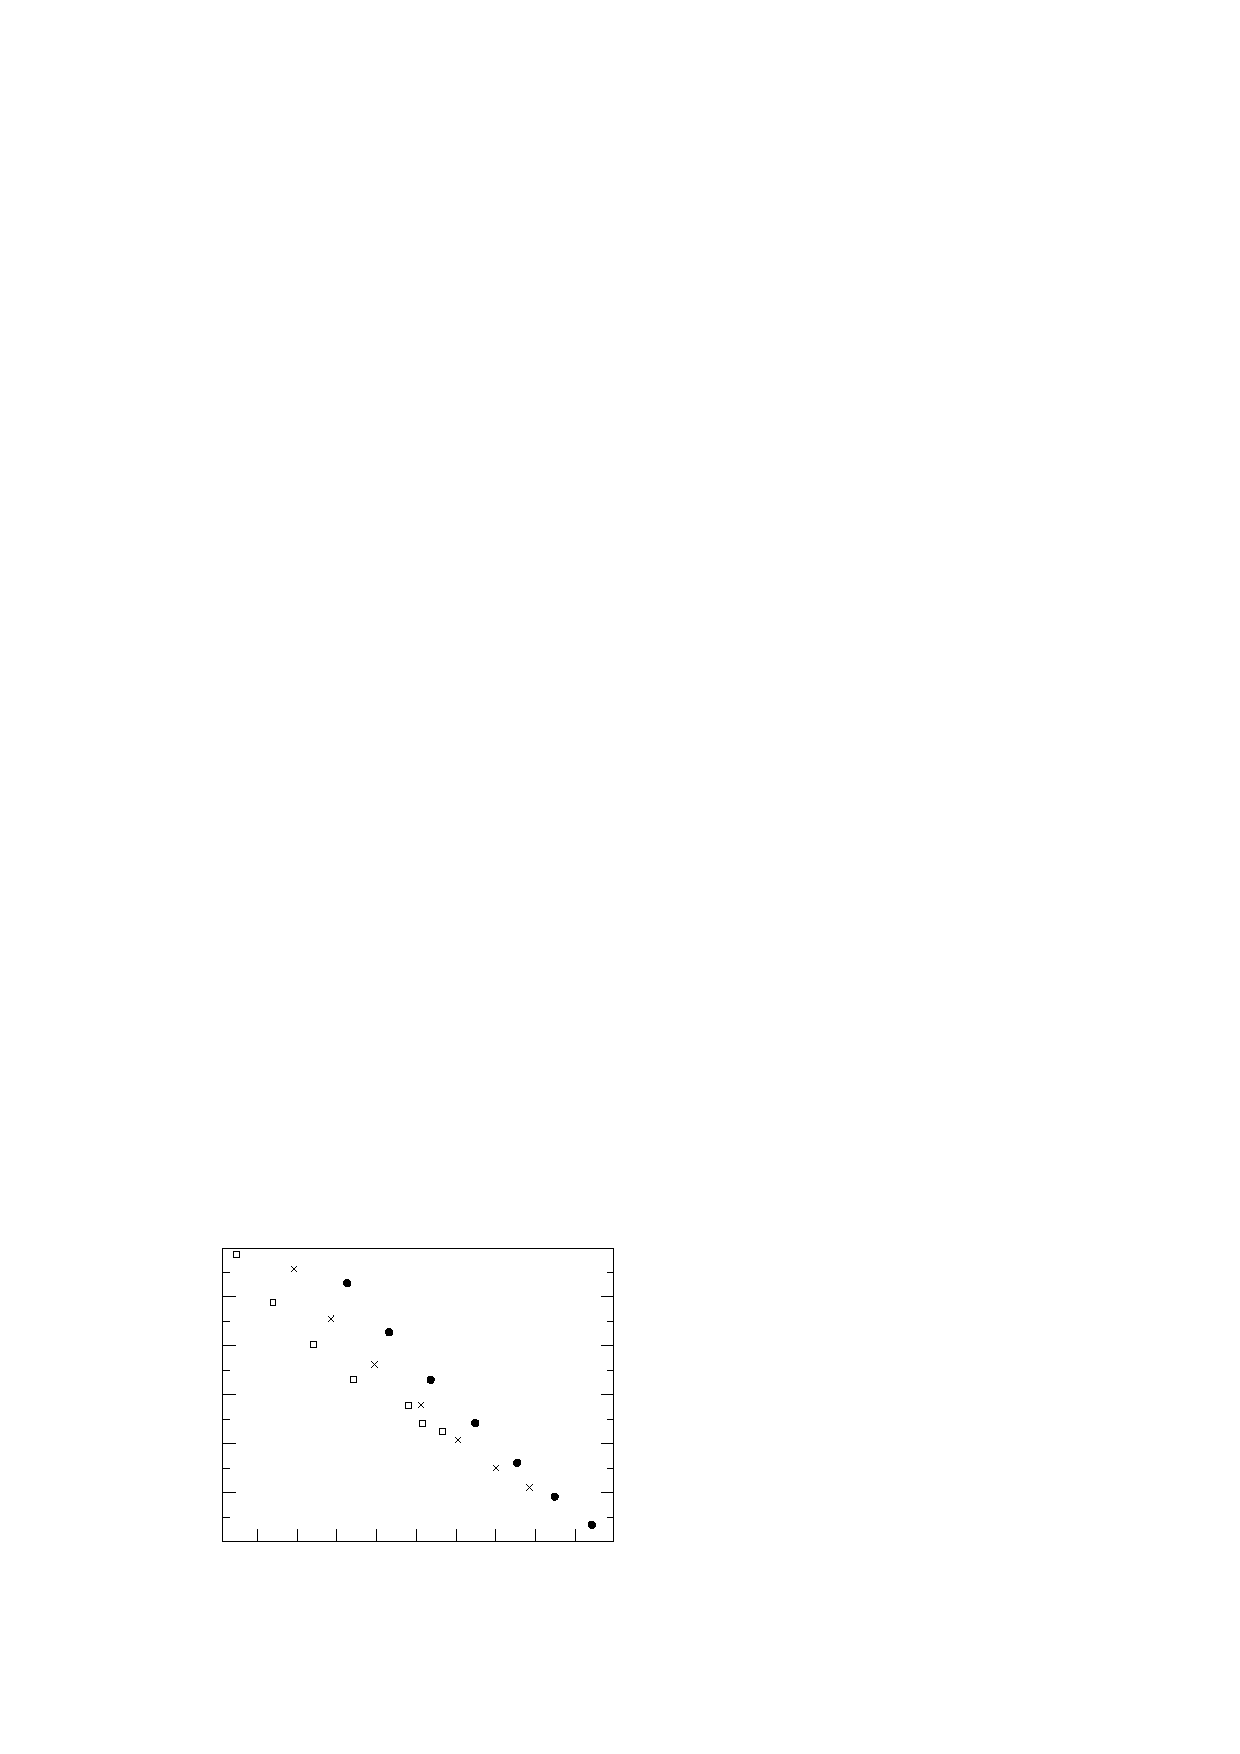
\includegraphics{place/tradeoff/ci}
  }}
}\end{picture}
%%
\caption{\label{fig:greedy_tradeoff}
  Trade-off between solution quality and running time (in logarithmic scale)
  with the Greedy algorithm on random chips of dimensions $300 \times 300$
  ({\tiny $\boxdot$}), $500 \times 500$ ({\tiny $\times$}) and $800 \times 800$
  ({\scriptsize $\bullet$}). The number $Q$ of candidates per spot are $1.25$K,
  $2.5$K, 5K, 10K, 20K, 40K, and 80K (from left to right). Layouts are measured
  by normalized border length (left) and average conflict index (right).}
\end{figure}

\begin{table}[p!]\centering
\caption{\label{tab:greedy}
  Normalized border length (NBL) and average conflict index (ACI) of layouts
  produced by Greedy on random chips of various dimensions. The results of
  Row-Epitaxial on the same set of chips (Table~\ref{tab:reptx}) is shown for
  comparison. Running times in minutes.}
\footnotesize{
\begin{tabular*}{\hsize}{crrrrrlrrrr}
\vspace{1pt}
     &         & \multicolumn{4}{c}{Border length minimization} & & \multicolumn{4}{c}{Conflict index minimization} \\ \cline{3-6} \cline{8-11}
\vspace{1pt}
     &         & \multicolumn{2}{c}{Row-Epitaxial} & \multicolumn{2}{c}{Greedy} & & \multicolumn{2}{c}{Row-Epitaxial} & \multicolumn{2}{c}{Greedy} \\
\vspace{1pt}
Dim. & $Q$ $k$ & NBL & Time & NBL & Time & & ACI & Time & ACI & Time \\
\hline
$300^2$ &  5K 0 & {\bf 18.2935} &  1.1 & {\bf 18.3182} &  1.6 &  &      462.5194  &   4.9 & {\bf 440.5166} &   5.4 \\
        &     1 &      18.2999  &  1.3 &      18.5037  &  1.6 &  & {\bf 462.4656} &   5.1 &      444.7837  &   5.3 \\
        &     2 &      18.3072  &  1.2 &      18.4222  &  1.6 &  &      462.6394  &   4.6 &      446.8662  &   5.3 \\
        &     3 &      18.3226  &  1.2 &      18.3863  &  1.6 &  &      462.5885  &   5.1 &      447.7464  &   5.0 \\
        &     4 &      18.3279  &  1.3 &      18.3728  &  1.5 &  &      462.7775  &   5.1 &      447.6559  &   5.3 \\
\cline{2-11}
        & 10K 0 & {\bf 18.1477} &  2.8 & {\bf 18.1830} &  4.3 &  &      444.0354  &   9.7 & {\bf 426.3480} &  10.9 \\
        &     1 &      18.1529  &  2.8 &      18.3912  &  4.7 &  &      444.0904  &   9.3 &      429.5617  &  11.3 \\
        &     2 &      18.1519  &  2.9 &      18.3058  &  4.5 &  &      444.1960  &  10.0 &      431.7555  &  11.1 \\
        &     3 &      18.1591  &  2.8 &      18.2732  &  4.6 &  & {\bf 443.9850} &  10.6 &      432.6821  &  11.3 \\
        &     4 &      18.1603  &  2.9 &      18.2415  &  4.6 &  &      444.1745  &   9.8 &      432.3800  &  11.0 \\
\cline{2-11}
        & 20K 0 &      18.0274  &  7.2 & {\bf 18.0576} &  9.6 &  &      426.7824  &  18.9 & {\bf 415.5003} &  30.3 \\
        &     1 &      18.0325  &  6.9 &      18.2813  &  9.2 &  &      426.8863  &  18.5 &      418.2357  &  21.3 \\
        &     2 &      18.0277  &  6.6 &      18.1985  &  9.2 &  &      426.8832  &  19.3 &      419.4866  &  21.1 \\
        &     3 & {\bf 18.0272} &  6.6 &      18.1617  &  9.5 &  &      426.8694  &  19.6 &      420.7345  &  20.1 \\
        &     4 &      18.0321  &  7.5 &      18.1328  &  8.8 &  & {\bf 426.6600} &  20.2 &      420.7332  &  21.0 \\
\hline
$500^2$ &  5K 0 & {\bf 17.6000} &  4.3 & {\bf 17.5830} &  5.8 &  &      456.2042  &  15.2 & {\bf 432.3023} &  15.9 \\
        &     1 &      17.6095  &  4.1 &      17.7842  &  5.3 &  & {\bf 456.1341} &  15.2 &      437.2417  &  16.2 \\
        &     2 &      17.6246  &  4.3 &      17.7087  &  5.3 &  &      456.5261  &  14.1 &      439.7432  &  15.6 \\
        &     3 &      17.6474  &  3.8 &      17.6759  &  5.4 &  &      456.5337  &  14.1 &      441.3441  &  16.2 \\
        &     4 &      17.6670  &  3.7 &      17.6561  &  5.4 &  &      456.8203  &  15.3 &      441.0668  &  16.1 \\
\cline{2-11}
        & 10K 0 & {\bf 17.4503} & 13.1 & {\bf 17.4673} & 15.8 &  &      438.7075  &  33.9 & {\bf 415.6951} &  35.4 \\
        &     1 &      17.4523  & 12.8 &      17.6765  & 16.0 &  &      438.7379  &  33.6 &      419.7788  &  33.4 \\
        &     2 &      17.4582  & 12.7 &      17.5936  & 16.8 &  & {\bf 438.6477} &  30.4 &      422.1943  &  36.3 \\
        &     3 &      17.4685  & 12.5 &      17.5550  & 16.2 &  &      438.8183  &  30.8 &      424.0554  &  34.6 \\
        &     4 &      17.4755  & 12.5 &      17.5324  & 15.7 &  &      438.9280  &  32.8 &      423.7936  &  35.2 \\
\cline{2-11}
        & 20K 0 &      17.3303  & 28.2 & {\bf 17.3554} & 33.3 &  &      421.1358  &  66.7 & {\bf 401.4609} &  67.1 \\
        &     1 & {\bf 17.3297} & 29.0 &      17.5829  & 34.0 &  &      421.1580  &  63.6 &      404.9949  &  69.8 \\
        &     2 &      17.3308  & 27.4 &      17.4939  & 34.1 &  &      421.1087  &  67.7 &      406.9576  &  67.8 \\
        &     3 &      17.3344  & 27.4 &      17.4519  & 34.7 &  & {\bf 420.9758} &  65.1 &      408.5048  &  69.4 \\
        &     4 &      17.3376  & 27.7 &      17.4273  & 33.7 &  &      421.0436  &  64.2 &      408.4556  &  68.4 \\
\hline
$800^2$ &  5K 0 & {\bf 16.9760} & 12.2 & {\bf 16.9124} & 15.3 &  & {\bf 448.0140} &  36.9 & {\bf 426.0757} &  41.9 \\
        &     1 &      16.9927  & 12.2 &      17.1259  & 15.5 &  &      448.1474  &  40.3 &      430.9759  &  42.7 \\
        &     2 &      17.0187  & 11.7 &      17.0551  & 15.1 &  &      448.6130  &  38.6 &      433.8504  &  42.9 \\
        &     3 &      17.0589  & 11.7 &      17.0214  & 15.4 &  &      448.9159  &  40.2 &      435.4797  &  43.3 \\
        &     4 &      17.1085  & 12.0 &      17.0009  & 15.4 &  &      449.1653  &  40.0 &      435.2589  &  43.2 \\
\cline{2-11}
        & 10K 0 & {\bf 16.8032} & 37.0 & {\bf 16.7951} & 45.5 &  & {\bf 432.2283} &  88.2 & {\bf 408.3982} &  91.4 \\
        &     1 &      16.8111  & 39.1 &      17.0122  & 43.2 &  &      432.5153  &  91.4 &      412.9971  &  95.1 \\
        &     2 &      16.8235  & 37.7 &      16.9333  & 45.1 &  &      432.5031  &  85.8 &      415.7934  &  91.7 \\
        &     3 &      16.8353  & 37.7 &      16.8935  & 45.9 &  &      432.6652  &  90.1 &      417.5229  &  95.2 \\
        &     4 &      16.8622  & 39.0 &      16.8748  & 45.6 &  &      432.6980  &  91.9 &      417.5098  &  91.3 \\
\cline{2-11}
        & 20K 0 & {\bf 16.6771} & 83.1 & {\bf 16.6980} & 95.8 &  & {\bf 415.6470} & 174.2 & {\bf 392.1786} & 186.4 \\
        &     1 &      16.6803  & 83.2 &      16.9263  & 93.2 &  &      415.7402  & 181.1 &      396.3923  & 185.9 \\
        &     2 &      16.6851  & 83.4 &      16.8376  & 93.8 &  &      415.6622  & 179.7 &      399.0043  & 186.9 \\
        &     3 &      16.6915  & 86.5 &      16.7947  & 94.4 &  &      415.7609  & 172.3 &      400.7189  & 183.3 \\
        &     4 &      16.7007  & 80.3 &      16.7727  & 97.2 &  &      415.7951  & 190.9 &      400.7257  & 189.3 \\
\hline
\end{tabular*}}
\end{table}

It should be noted that, like Row-Epitaxial, Greedy has the drawback of treating
the last spots of a chip ``unfairly'': While $Q$ probe candidades are examined
for each of the first $n - Q + 1$ filled spots, the last $Q - 1$ spots have
fewer than $Q$ candidates (in particular, when the last spot is being filled,
there is only one probe candidate). As a result, we usually observe
comparatively higher levels of conflicts in the last filled spots.

We also observed that, in terms of border length, increasing $Q$ above 5K has
little positive effect (see Figure~\ref{fig:greedy_tradeoff}). For instance, on
$800\times 800$ chips, increasing $Q$ from 5K to 20K reduced the normalized
border length by only $1.27\%$ (from $16.9124$ to $16.6980$ with $k=0$), while
requiring approximately six times more time. In terms of conflict index,
however, increasing $Q$ even above 40K still results in significant improvements
for large chips. For instance, on $800\times 800$ chips, increasing $Q$ from 40K
to 80K reduced the average conflict index by $3.18\%$ (from $378.3110$ to
$366.8446$ with $k=0$, data not shown). The fact that increasing $Q$ has more
effect in terms of conflict index is probably because, in this measure, there is
more room for optimization as the conflicts can be moved to the extremities of
the probes (while retaining the same number of border conflicts) and a larger
number of neighbors are involved.

Figure~\ref{fig:greedy_blm} shows the normalized border length per masking step
of layouts produced by Greedy for a $500\times 500$ chip with border length and
conflict index minimization. With BLM, the generated layout has most border
conflicts concentrated between steps 7 and 58. The last masks of this layout
have low levels of border conflicts because the probes are left-most embedded,
which leaves most embeddings in an unproductive state during the final synthesis
steps. As a result of the lexicographical sorting of probes, the first masks
also have relatively few conflicts. A representation of selected
photolithographic masks for this layout are shown in Figure
\ref{fig:greedy-bl_masks}. Layers of masked and unmasked regions that result
from sorting probes lexicographically can be seen in masks $M_1$ to $M_8$.
Masks $M_9$ to $M_{62}$ are very ``noisy'' as there seems to be little
regularity in their arrangement. After $M_{62}$, masks start to get ``darker''
as most probes have been already fully synthesized.

With CIM, Greedy shifts border conflicts away from the steps that add the
middle bases (between steps 20 and 45; see Figure~\ref{fig:greedy_blm}),
which effectively reduces the average conflict index. Not surprisingly, this
reduction comes at the expense of an increase in total border length --- the
normalized border length of this particular chip rose from $17.3513$ with BLM to
$19.8461$ with CIM. Figure~\ref{fig:greedy-ci_masks} shows a representation of
selected masks for this layout. Note that the first masks ($M_1$ to $M_4$)
still exhibit a ``layered'' structured, althought the layers are much narrower
and the masks noisier than the first masks of Figure~\ref{fig:greedy-bl_masks}.
In the central masks $M_{20}$ to $M_{45}$, especially between $M_{25}$ and
$M_{40}$, it is possible to see clusters of masked and unmasked spots that cause
the reduction in average conflict index.

\begin{figure}[t]\centering
\includegraphics{place/greedymasks/bl}
\caption{\label{fig:greedy_blm}%
  Normalized border length (on the left y-axis) per masking step
  of layouts produced by Greedy for a $500\times 500$ chip with border length
  ({\tiny $\times$}) and conflict index ({\tiny $\boxdot$}) minimization using
  $0$-threading and $Q=20$K. Chip contained random probe sequences left-most
  embedded in the standard 74-step Affymetrix deposition sequence. The number of
  middle bases synthesized at each step is shown in boxes (right y-axis).}
\end{figure}

\begin{figure}[p]\centering
%%
\begin{picture}(435,567)\footnotesize{
\put( -2,439){\makebox(145,128){\includegraphics{place/greedymasks/bl/mask01}}}
\put(147,439){\makebox(145,128){
\includegraphics{place/greedymasks/bl/mask02}}}
\put(292,439){\makebox(145,128){
\includegraphics{place/greedymasks/bl/mask03}}}
\put( -2,429){\makebox(145, 10){$M_1$}}
\put(147,429){\makebox(145, 10){$M_2$}}
\put(292,429){\makebox(145, 10){$M_3$}}
\put( -2,296){\makebox(145,128){\includegraphics{place/greedymasks/bl/mask04}}}
\put(147,296){\makebox(145,128){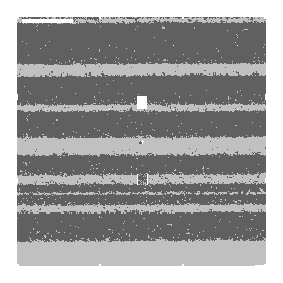
\includegraphics{place/greedymasks/bl/mask05}}}
\put(292,296){\makebox(145,128){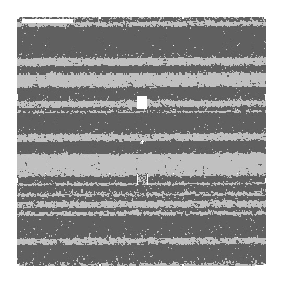
\includegraphics{place/greedymasks/bl/mask06}}}
\put( -2,286){\makebox(145, 10){$M_4$}}
\put(147,286){\makebox(145, 10){$M_5$}}
\put(292,286){\makebox(145, 10){$M_6$}}
\put( -2,153){\makebox(145,128){
\includegraphics{place/greedymasks/bl/mask07}}}
\put(147,153){\makebox(145,128){
\includegraphics{place/greedymasks/bl/mask08}}}
\put(292,153){\makebox(145,128){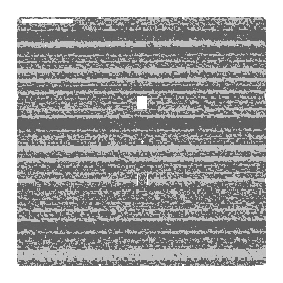
\includegraphics{place/greedymasks/bl/mask09}}}
\put( -2,143){\makebox(145, 10){$M_7$}}
\put(147,143){\makebox(145, 10){$M_8$}}
\put(292,143){\makebox(145, 10){$M_9$}}
\put( -2, 10){\makebox(145,128){\includegraphics{place/greedymasks/bl/mask62}}}
\put(147, 10){\makebox(145,128){
\includegraphics{place/greedymasks/bl/mask70}}}
\put(292, 10){\makebox(145,128){\includegraphics{place/greedymasks/bl/mask74}}}
\put( -2,  0){\makebox(145, 10){$M_{62}$}}
\put(147,  0){\makebox(145, 10){$M_{70}$}}
\put(292,  0){\makebox(145, 10){$M_{74}$}}
}\end{picture}
%%
\caption{\label{fig:greedy-bl_masks}%
  Selected masks generated by Greedy with border length minimization for a
  random $500\times 500$ chip with 25-mer probes left-most embedded in the
  standard Affymetrix deposition sequence. Unmasked (masked) spots are
  represented by light (dark) dots.}
\end{figure}

\begin{figure}[p]\centering
%%
\begin{picture}(435,567)\footnotesize{
\put( -2,439){\makebox(145,128){\includegraphics{place/greedymasks/ci/mask01}}}
\put(147,439){\makebox(145,128){
\includegraphics{place/greedymasks/ci/mask02}}}
\put(292,439){\makebox(145,128){
\includegraphics{place/greedymasks/ci/mask03}}}
\put( -2,429){\makebox(145, 10){$M_1$}}
\put(147,429){\makebox(145, 10){$M_2$}}
\put(292,429){\makebox(145, 10){$M_3$}}
\put( -2,296){\makebox(145,128){\includegraphics{place/greedymasks/ci/mask04}}}
\put(147,296){\makebox(145,128){\includegraphics{place/greedymasks/ci/mask20}}}
\put(292,296){\makebox(145,128){
\includegraphics{place/greedymasks/ci/mask25}}}
\put( -2,286){\makebox(145, 10){$M_4$}}
\put(147,286){\makebox(145, 10){$M_{20}$}}
\put(292,286){\makebox(145, 10){$M_{25}$}}
\put( -2,153){\makebox(145,128){\includegraphics{place/greedymasks/ci/mask30}}}
\put(147,153){\makebox(145,128){
\includegraphics{place/greedymasks/ci/mask32}}}
\put(292,153){\makebox(145,128){\includegraphics{place/greedymasks/ci/mask37}}}
\put( -2,143){\makebox(145, 10){$M_{30}$}}
\put(147,143){\makebox(145, 10){$M_{32}$}}
\put(292,143){\makebox(145, 10){$M_{37}$}}
\put( -2, 10){\makebox(145,128){\includegraphics{place/greedymasks/ci/mask40}}}
\put(147, 10){\makebox(145,128){\includegraphics{place/greedymasks/ci/mask45}}}
\put(292, 10){\makebox(145,128){\includegraphics{place/greedymasks/ci/mask65}}}
\put( -2,  0){\makebox(145, 10){$M_{40}$}}
\put(147,  0){\makebox(145, 10){$M_{45}$}}
\put(292,  0){\makebox(145, 10){$M_{65}$}}
}\end{picture}
%%
\caption{\label{fig:greedy-ci_masks}%
  Selected masks generated by Greedy with conflict index minimization for a
  random $500\times 500$ chip with 25-mer probes left-most embedded in the
  standard Affymetrix deposition sequence. Unmasked (masked) spots are
  represented by light (dark) dots.}
\end{figure}

%%%%%%%%%%%%%%%%%%%%%%%%%%%%%%%%%%%%%%%%%%%%%%%%%%%%%%%%%%%%%%%%%%%%%%%%%%%%%%%%
\section{Summary}
\label{sec:placement_summary}

In this chapter, we have surveyed placement algorithms for the microarray layout
problem, including an optimal placement strategy for uniform arrays based on a
two-dimensional Gray code, an approach based on the traveling salesman problem
and different threading techniques. For general arrays, we have presented more
experimental results with Row-Epitaxial, the best known placement algorithm to
date, and studied the impact of the choice of threading for its initial layout.

We have also introduced a new placement algorithm, called Greedy. Greedy
achieved similar results in terms of BLM and better results in terms of CIM
compared to Row-Epitaxial. For BLM, Row-Epitaxial is faster than Greedy and
should still be the method of choice. For CIM, however, the improvements
achieved by Greedy over Row-Epitaxial justify the small increase in running
time.

%%%%%%%%%%%%%%%%%%%%%%%%%%%%%%%%%%%%%%%%%%%%%%%%%%%%%%%%%%%%%%%%%%%%%%%%%%%%%%%%
\chapter{MLP and the Quadratic Assignment Problem}
\label{ch:qap}
%%%%%%%%%%%%%%%%%%%%%%%%%%%%%%%%%%%%%%%%%%%%%%%%%%%%%%%%%%%%%%%%%%%%%%%%%%%%%%%%

In this chapter, we show that the Microarray Placement Problem (MLP) with
general distance-dependent and position-dependent weights is an instance of the
\emph{Quadratic Assignment Problem} (QAP), a classical combinatorial
optimization problem introduced by~\citet{Koopmans1957}, which opens up the way
for using QAP techniques to design microarray chips.

We then use an existing QAP heuristic algorithm called GRASP to design the
layout of small artificial chips, comparing our results with the best known
placement algorithm. The chapter ends with a discussion about how this approach
can be combined with other existing algorithms to design and improve larger
microarrays.

%%%%%%%%%%%%%%%%%%%%%%%%%%%%%%%%%%%%%%%%%%%%%%%%%%%%%%%%%%%%%%%%%%%%%%%%%%%%%%%%
\section{Quadratic assignment problem}
\label{sec:qap_qap}

The quadratic assignment problem (QAP) can be stated as follows. Given
$n \times n$ real-valued matrices $F = (f_{ij})\geq 0$ and $D = (d_{kl})\geq 0$,
find a permutation $\pi$ of $\{1, 2, \ldots n\}$ such that
\begin{equation}\label{eq:qap_def}
  \sum_{i=1}^{n} \sum_{j=1}^{n}\,  f_{ij} \cdot d_{\pi(i)\pi(j)} \to \min.
\end{equation}

The attribute \emph{quadratic} stems from the fact that the target function can
be written with $n^2$ binary indicator variables $x_{ik}\in\{0,1\}$, where
$x_{ik}:=1$ if and only if $k=\pi(i)$. The objective~(\ref{eq:qap_def}) then
becomes
%%
\[
  \sum_{i=1}^{n} \sum_{j=1}^{n}\,  f_{ij} \cdot 
  \sum_{k=1}^{n} \sum_{l=1}^{n}\,  d_{kl} \cdot x_{ik}\cdot x_{jl}
  \to \min,
\]
%%
such that $\sum_{k}\, x_{ik}=1$ for all $i$, $\sum_{i}\, x_{ik}=1$ for all $k$,
and $x_{ik}\in\{0,1\}$ for all $(i,k)$. The objective function is a quadratic
form in $x$.

The QAP has been used to model a variety of real-life problems. One common
example is the facility location problem where $n$ facilities must be assigned
to $n$ locations. The facilities could be, for instance, the clinics, doctors or
services (X-ray, emergency room, etc.) provided by a hospital and the locations
could be the available rooms of the hospital building.

In this scenario, $F$ is called the \emph{flow matrix} as $f_{ij}$ represents
the flow of materials or persons from facility $i$ to facility $j$. Matrix $D$
is called the \emph{distance matrix}, as $d_{kl}$ gives the distance between
locations $k$ and $l$. One unit of flow is assumed to have an associated cost
proportional to the distance between the facilities, and the optimal permutation
$\pi$ defines a one-to-one assignment of facilities to locations with minimum
cost.

%%%%%%%%%%%%%%%%%%%%%%%%%%%%%%%%%%%%%%%%%%%%%%%%%%%%%%%%%%%%%%%%%%%%%%%%%%%%%%%%
\section{QAP formulation of the MLP}
\label{sec:qap_mlp}

The MLP can be seen as an instance of the QAP, where we want to find a
one-to-one correspondence between spots and probes minimizing a given penalty
funtion such as total border length or total conflict index (defined in Chapter
\ref{ch:mlp}). To formulate it, we use the facility location example by viewing
the probes as locations and the spots as facilities, i.e., the spots are
assigned to the probes. The flow matrix $F$ then contains the ``closeness''
values between spots, while the distance matrix $D$ contains the conflicts
between probe embeddings.

We first give the general formulation for conflict index minimization case; the
border length minimization case is obtained by using the particular weight
functions given in Section~\ref{sec:mlp_bl_vs_ci}.

In a realistic setting, we may have more spots available than probes to place.
Below, we show that this does not cause problems as we can add enough ``empty''
probes and define their weights appropriately.

Perhaps more severely, we assume that all probes have a single pre-defined
embedding in order to force a one-to-one relationship.  A more elaborate
formulation would consider all possible embeddings of a probe, but then it
becomes necessary to ensure that only one embedding of each probe is used. This
still leads to a quadratic integer programming problem, albeit with slightly
different side conditions.

Our goal is to design a microarray minimizing the sum of conflict indices over
all spots~$s \in \CalS$, i.e.,
%%
\[
\sum_{s \in \CalS} \mathcal{C}(s) \to \min.
\]

The ``flow'' $f_{ij}$ between spots $i$ and $j$ depends on their distance on the
chip; in accordance with the conflict index model, we set
%%
\begin{equation}
  f_{ij} := \Ind{i,j \text{ neighbors}} \cdot \gamma(i,j)
\end{equation}
%%
where ``neighbors'' means that spots $i$ and $j$ are at most three cells away
(horizontally and vertically) from each other. Note that most of the flow values
on large arrays are zero. For border length minimization, the case is even
simpler: We set $f_{ij}:=1$ if spots $i$ and $j$ are adjacent, and $f_{ij}:=0$
otherwise.

The ``distance'' $d_{kl}$ between probes $k$ and $l$ depends on the conflicts
between their embeddings $\eps_k$ and $\eps_l$. To account for possible
``empty'' probes to fill up surplus spots, we set $d_{kl}:=0$ if $k$ or $l$ or
both refer to an empty probe --- i.e., empty probes never contribute to the
target function since we do not mind if nucleotides are erroneously synthesized
on spots assigned to empty probes. For real probes, we set
%%
\begin{equation}
  d_{kl} := \sum_{t=1}^{T} \Bigl(
    \Ind{\eps_{k,t}=0}
    \cdot \omega(\eps_k,t)
    \cdot \Ind{\eps_{l,t}=1} \Bigr).
\end{equation}

Note that $d_{kl}$ is related to the conflict index distance $C(k,l)$ defined in
Section~\ref{sec:mlp_conflict_index} (Eq.~\ref{eq:ci_dist}):
%%
\begin{eqnarray*}
 &   & d_{kl} + d_{lk} \\
 & = & \sum_{t=1}^{T} \Bigl( \Ind{\eps_{k,t}=0} \cdot \omega(\eps_k,t) \cdot \Ind{\eps_{l,t}=1} \Bigr)
     + \sum_{t=1}^{T} \Bigl( \Ind{\eps_{l,t}=0} \cdot \omega(\eps_l,t) \cdot \Ind{\eps_{k,t}=1} \Bigr) \\
 & = & \sum_{t=1}^{T} \Bigl( \Ind{\eps_{k,t}=0 \text{ and } \eps_{l,t}=1} \cdot \omega(\eps_k,t) \Bigr)
     + \sum_{t=1}^{T} \Bigl( \Ind{\eps_{l,t}=0 \text{ and } \eps_{k,t}=1} \cdot \omega(\eps_l,t) \Bigr) \\
 & = & \sum_{t=1}^{T} \Bigl(
                        \Ind{\eps_{k,t}=0 \text{ and } \eps_{l,t}=1} \cdot \omega(\eps_k,t) +
                        \Ind{\eps_{l,t}=0 \text{ and } \eps_{k,t}=1} \cdot \omega(\eps_l,t)
                      \Bigr) \\
 & = & C(k,l)
\end{eqnarray*}

In the case of border length minimization, where $\theta=0$ and $c=1/2$ (see
Section~\ref{sec:mlp_bl_vs_ci}), we obtain that
$d_{kl} + d_{lk} = H(k,l) = H(l,k)$, where $H_{kl}$ denotes the Hamming distance
between the embeddings $\eps_k$ and $\eps_l$ (Eq.~\ref{eq:hamming}).

It now follows that for a given assignment $\pi$, we have,
%%
\[
f_{ij} \cdot d_{\pi(i)\pi(j)} = \sum_{t=1}^{T} \Bigl(
  \Ind{\eps_{\pi(i),t}=0}
  \cdot \omega(\eps_{\pi(i)},t)
  \cdot \Ind{\eps_{\pi(j),t}=1}
  \cdot \Ind{i,j \text{ neighbors}}
  \cdot \gamma(i,j) \Bigr).
\]

The objective function~(\ref{eq:qap_def}) then becomes
%%
\begin{eqnarray*}
 &   & \sum_i \sum_j\, f_{ij} \cdot d_{\pi(i)\pi(j)} \\
 & = & \sum_i \sum_j\, \sum_{t=1}^{T}
                       \Bigl(
                         \Ind{\eps_{\pi(i),t}=0}
                         \cdot \omega(\eps_{\pi(i)},t)
                         \cdot \Ind{\eps_{\pi(j),t}=1}
                         \cdot \Ind{i,j \text{ neighbors}}
                         \cdot \gamma(i,j)
                       \Bigr) \\
 & = & \sum_i \sum_{t=1}^T\,
              \Bigl(
                 \Ind{\eps_{\pi(i),t}=0}
                 \cdot \omega(\eps_{\pi(i)},t)
                 \cdot \sum_j\,
                 \Ind{i,j \text{ neighbors}}
                 \cdot \Ind{\eps_{\pi(j),t}=1}
                 \cdot \gamma(i,j)
              \Bigr) \\
 & = & \sum_i \sum_{t=1}^T\,
              \Bigl(
                 \Ind{\eps_{\pi(i),t}=0}
                 \cdot \omega(\eps_{\pi(i)},t)
                 \cdot \sum_{\substack{j \text{: neighbor}\\\text{of } i}}\,
                 \Ind{\eps_{\pi(j),t}=1}
                 \cdot \gamma(i,j)
              \Bigr) \\
 & = & \sum_i \mathcal{C}(i), \\
\end{eqnarray*}
%%
and indeed equals the total conflict index with our definitions of $F=(f_{ij})$
and $D=(d_{kl})$.

\paragraph{Remark.}
Note that it is technically possible to switch the definitions of $F$ and $D$,
i.e., to assign probes to spots instead of spots to probes as we do now, without
modifying the mathematical problem formulation. However, this would lead to high
distance values for neighboring spots and many zero distance values for
independent spots, a somewhat counterintuitive model. Also, some QAP heuristics
initially find pairs of objects with large flow values and place them close to
each other. Therefore, the way of modeling $F$ and $D$ may be significant.

%%%%%%%%%%%%%%%%%%%%%%%%%%%%%%%%%%%%%%%%%%%%%%%%%%%%%%%%%%%%%%%%%%%%%%%%%%%%%%%%
\section{QAP heuristics}
\label{sec:qap_heuristics}

We have shown how the microarray placement problem can be modeled as a
quadratic assignment problem. However, the QAP is known to be NP-hard and
particularly hard to solve in practice. Instances of size larger than
$n = 20$ are generally considered to be impossible to solve to
optimality. Fortunately, several heuristics exist, including approaches based on
tabu search, simulated annealing and genetic algorithms
\citep[for a survey, see][]{Cela1997}. Our formulation is thus of interest
because we can now use existing QAP heuristics to design the layout of
microarrays minimizing either the sum of border lengths or conflict indices.

As an example, we briefly describe a general QAP heuristic known as GRASP \citep
{Li1994}, which was first used for solving the QAP by \citet{Feo1995}, and an
improved version called GRASP with path-relinking \citep{Oliveira2004}, that we
used to design small microarray chips with our formulation.

\subsection{GRASP with Path-relinking}
\label{sec:qap_grasp}

GRASP (Greedy Randomized Adaptive Search Procedure) is comprised of two phases:
a construction phase where a random feasible solution is built, and a local
search phase where a local optimum in the neighborhood of that solution is
sought. In the following description we use the terms of the facility location
problem: $f_{ij}$ is the flow between facilities $i$ and $j$, $d_{kl}$ is the
distance between locations $k$ and $l$.

The construction phase starts by sorting the $(n^2 - n)$ elements of the
distance matrix in increasing order and keeping the smallest
$E:= \lfloor \beta (n^2 - n) \rfloor$ elements, where $0 < \beta < 1$ is a
restriction parameter given as input.
%%
\begin{displaymath}
d_{k_1 l_1} \le d_{k_2 l_2} \le \cdots \le d_{k_E l_E}.
\end{displaymath}

Similarly, the $(n^2 - n)$ elements of the flow matrix are sorted, this time in
decreasing order, and the largest $E$ elements are kept:
%%
\begin{displaymath}
f_{i_1 j_1} \ge f_{i_2 j_2} \ge \cdots \ge f_{i_E j_E}.
\end{displaymath}

Then, the costs of assigning pairs of facilities to pairs of locations are
computed. The cost of initially assigning facility $i_q$ to location $k_q$ and
facility $j_q$ to location $l_q$ for some $q\in\{1,\ldots,E\}$ is
$d_{k_q l_q} f_{i_q j_q}$. GRASP sorts the vector
%%
\begin{displaymath}
(d_{k_1 l_1} f_{i_1 j_1},\;
 d_{k_2 l_2} f_{i_2 j_2},\; \ldots,\;
 d_{k_E l_E} f_{i_E j_E}),
\end{displaymath}
%%
keeping the $\lfloor \alpha E \rfloor$ smallest elements, where $0 < \alpha < 1$
is another restriction parameter. A simultaneous assignment of a pair of
facilities to a pair of locations is selected at random among those with the
$\lfloor \alpha E \rfloor$ smallest costs, and a feasible solution is then built
by making a series of greedy assignments.

In the local search phase, GRASP searches for a local optimum in the
neighborhood of the constructed solution. Several search strategies and
definitions of neighborhood can be used. One possible approach is to check every
possible swap of assignments and make only those which improve the current
solution until no further improvements can be made.

The construction and local search phases are repeated for a given number of
times, and the best solution found is returned.

\paragraph{Path-relinking.}
GRASP takes no advantage of the knowledge gained in previous iterations to
build or improve an obtained solution, i.e., each new solution is built from
scratch.

GRASP with path-relinking is an extension of the basic GRASP algorithm that uses
an ``elite set'' to store the best solutions found. It incorporates a third
phase that chooses, at random, one elite solution that is used to improve the
solution produced at the end of the local search phase.

Solutions $p$ and $q$ are combined as follows. For every location
$k = 1, \ldots, n$, the path-relinking algorithm attempts to exchange facility
$p_k$ assigned to location $k$ in  solution $p$ with facility $q_k$ assigned to
location $k$ in the elite solution. In order to keep the solution $p$ feasible,
it exchanges $p_k$ with $p_l$, where $p_l = q_k$. This exchange is performed
only if it results in a better solution. The result of the path-relinking phase
is a solution $r$ that is at least as good as the better of $p$ and $q$.

%%%%%%%%%%%%%%%%%%%%%%%%%%%%%%%%%%%%%%%%%%%%%%%%%%%%%%%%%%%%%%%%%%%%%%%%%%%%%%%%
\section{Results}
\label{sec:qap_results}

We present experimental results of using GRASP with path-relinking (GRASP-PR)
for designing the layout of small artificial chips, and compare them with the
layouts produced by Row-Epitaxial (described in Chapter \ref{ch:placement}).

We used a C implementation of GRASP-PR provided by \citet{Oliveira2004} with
default parameters (32 iterations, $\alpha=0.1$, $\beta=0.5$, and elite set of
size $10$). The main routine takes three arguments: the dimension $n$ of the
problem (in our case, the number of spots or probes) and matrices $F$ and $D$.
The matrices were generated using the formulations presented in Section
\ref{sec:qap_mlp}.

The data set consists of chips with probes of length 25 uniformly generated and
asynchronously embedded in a deposition sequence of length 74. The running times
and the border lengths of the resulting layouts are shown in
Table~\ref{tab:graspr_reptx_bl} (all results are averages over a set of ten
chips).

\begin{table}[t]\centering
\caption{\label{tab:graspr_reptx_bl}
  Border length of random chips compared with the layouts produced by
  Row-Epitaxial and GRASP with path-relinking. Reductions in border length are
  reported in percentages compared to the random layout.}
\small{
\begin{tabular*}{\hsize}{crcrrrcrrr}
          & Random & & \multicolumn{3}{c}{Row-Epitaxial}  & & \multicolumn{3}{c}{GRASP with path-relinking}  \\ \cline{2-2} \cline{4-6} \cline{8-10}
Chip      & Border & & Border & Reduction & Time          & & Border & Reduction & Time   \\
dimension & length & & length & (\%)      & (sec.)        & & length & (\%)      & (sec.) \\
\hline
$6\times 6$   & 1\,989.20 & & 1\,714.60 & 13.80 & 0.01 & & 1\,672.20 & 15.94 &   2.73 \\
$7\times 7$   & 2\,783.20 & & 2\,354.60 & 15.40 & 0.02 & & 2\,332.60 & 16.19 &   6.43 \\
$8\times 8$   & 3\,721.20 & & 3\,123.80 & 16.05 & 0.03 & & 3\,099.13 & 16.72 &  12.49 \\
$9\times 9$   & 4\,762.00 & & 3\,974.80 & 16.53 & 0.05 & & 3\,967.20 & 16.69 &  25.96 \\
$10\times 10$ & 5\,985.20 & & 4\,895.60 & 18.20 & 0.06 & & 4\,911.40 & 17.94 &  47.57 \\
$11\times 11$ & 7\,288.40 & & 5\,954.40 & 18.30 & 0.10 & & 5\,990.73 & 17.80 &  87.48 \\
$12\times 12$ & 8\,714.00 & & 7\,086.20 & 18.68 & 0.11 & & 7\,159.80 & 17.84 & 152.42 \\
\hline
\end{tabular*}}
\end{table}

Our results show that GRASP-PR produces layouts with lower border lengths than
Row-Epitaxial on the smaller chips. On 6\,x\,6 chips, GRASP-PR outperforms
Row-Epitaxial by $2.14$ percentage points on average ($15.94\% - 13.80\%$), when
compared to the initial random layout. On 9\,x\,9 chips, however, this
difference drops to $0.16$ percentage points, while Row-Epitaxial generates
better layouts on 11\,x\,11 or larger chips. In terms of running time,
Row-Epitaxial is faster and shows little variation as the number of probes
grows. In contrast, the time required to compute a layout with GRASP-PR
increases at a fast rate.

Table~\ref{tab:graspr_reptx_ci} shows better results in terms of conflict
indices. GRASP-PR consistently produces better layouts on all chip dimensions,
achieving up to $6.38$\% less conflicts on 10\,x\,10 chips, for example, when
compared to Row-Epitaxial. In terms of running times, GRASP-PR is even slower
than in the border length case. The reason is not clear, but it could be related
to the fact that the distance matrix contains fewer zero entries with the
conflict index formulation.

The gains in terms of conflict index of both Row-Epitaxial and GRASP-PR are
clearly less than the gains in terms of border length (when compared to the
initial random layout). This may be because the embeddings are fixed and the
reduction of conflicts is restricted to the relocation of the probes, which only
accounts for one part of the conflict index model.

\begin{table}[t]
\caption{\label{tab:graspr_reptx_ci}
  Average conflict indices of random chips compared with the layouts produced by
  Row-Epitaxial and GRASP with path-relinking.}
\small{
\begin{tabular*}{\hsize}{crcrrrcrrr}
          & Random & & \multicolumn{3}{c}{Row-Epitaxial}  & & \multicolumn{3}{c}{GRASP with path-relinking}  \\ \cline{2-2} \cline{4-6} \cline{8-10}
Chip      & Avg. C.& & Avg. C.& Reduction & Time          & & Avg. C.& Reduction & Time   \\
dimension & Index  & & Index  & (\%)      & (sec.)        & & Index  & (\%)      & (sec.) \\
\hline
$6\times 6$   & 524.28 & & 495.15 & 5.56 & 0.05 & & 467.08 & 10.91 &   3.68 \\
$7\times 7$   & 558.25 & & 521.90 & 6.51 & 0.07 & & 489.32 & 12.35 &   8.84 \\
$8\times 8$   & 590.51 & & 551.84 & 6.55 & 0.09 & & 515.69 & 12.67 &  19.48 \\
$9\times 9$   & 613.25 & & 568.62 & 7.28 & 0.11 & & 533.79 & 12.96 &  38.83 \\
$10\times 10$ & 628.50 & & 576.49 & 8.28 & 0.11 & & 539.69 & 14.13 &  73.09 \\
$11\times 11$ & 642.72 & & 588.91 & 8.37 & 0.12 & & 551.41 & 14.21 & 145.67 \\
$12\times 12$ & 656.86 & & 598.21 & 8.93 & 0.12 & & 561.21 & 14.56 & 249.19 \\
\hline
\end{tabular*}}
\end{table}

%%%%%%%%%%%%%%%%%%%%%%%%%%%%%%%%%%%%%%%%%%%%%%%%%%%%%%%%%%%%%%%%%%%%%%%%%%%%%%%%
\section{Discussion}
\label{sec:qap_discussion}

The QAP is notoriously hard to solve, and currently known exact methods start to
take prohibitively long already for slightly more than $20$ objects, i.e., we
could barely solve the problem exactly for $5\times 5$ arrays. Fortunately, the
literature on QAP heuristics is rich, as many problems in operations research
can be modeled as QAPs. Here we used one such heuristic to identify the
potential of the MLP-QAP-relation.

As our results show, however, even heuristic algorithms are too slow to deal
with chips of dimensions larger than $12 \times 12$, and although we could
design a $20 \times 20$ chip with a QAP heuristic within a day, we have to keep
in mind that this would still be a very small part of bigger problem as real
microarray dimensions range from $200 \times 200$ up to $1164 \times 1164$.

For this reason, we restricted our experiments to such small chips and QAP
heuristics that could handle the problems within a few minutes. Up to now,
finding exact solutions even to these small microarrays seems to be an
incredible hard task. We mention here experiments conducted by Dr. Peter Hahn,
who used two branch-and-bound algorithms to solve some problem instances from
Table \ref{tab:graspr_reptx_bl}. With RTL-2 \citep{Adams}, it was possible to
find two solutions with total border length of $1\,652$ for a selected
$6\times 6$ chip, being only $1.43\%$ better than the solution found with GRASP-
PR ($1\,676$), although it took RTL-2 about $6.5$ hours, in contrast with the
less than 3 seconds needed by GRASP-PR. A lower bound calculation for the same
problem resulted in $1\,624$, so the RTL-2 solution is only $1.69\%$ higher,
while the gap to the GRASP-PR solution is about $3.10\%$.

For another selected problem of dimension $7\times 7$, Dr. Hahn found one
solution with border length $2\,290$ using RTL-1 \citep{Hahn1998}, being about
$1.72\%$ better than the solution found by GRASP-PR ($2\,330$), although it took
RTL-1 some 29 hours, in contrast with the less than 7 seconds needed for the
GRASP-PR run. The results obtained with exact QAP solvers give an idea of how
hard the quadratic assignment problem actually is, and show that the results
with GRASP-PR are a good compromise when time is limited.

Improved results for several selected problem instances from Tables
\ref{tab:graspr_reptx_bl} and \ref{tab:graspr_reptx_ci} were also reported by
Chris MacPhee using GATS, a hybrid genetic / tabu search algorithm, although
these results were obtained on a number of large memory SMP machines, each
having 144 processors and 576 GB of global memory. The latest results for these
selected problems are available online at \url{
http://gi.cebitec.uni-bielefeld.de/assb/chiplayout/qap}.

\subsection{Alternatives}

It is clear that, because of the large number of probes on industrial
microarrays, it is not feasible to use GRASP-PR (or any other currently
available QAP method) to design an entire microarray chip. However, we showed
that it is certainly possible to use it on small sub-regions of a chip, which
opens up the way for two alternatives.

First, the QAP approach could be used combined with a partitioning algorithm
such as those discussed in Chapter \ref{ch:part} to the design the smaller
regions that result from the partitioning. This, however, does not seem
promising because, as we will see later, a partitioning is a compromise in
solution quality, and level of partitioning required to achieve the dimensions
supported by the QAP approach is too high.

It is interesting to extrapolate the times shown on Table
\ref{tab:graspr_reptx_bl} to predict the total time that would be required to
design the layout of commercial microarrays, if we were to combine GRASP-PR with
a partitioning algorithm. If the partitioning produced $6\times 6$ regions,
$37\,636$ sub-regions would be created from the $1164\times 1164$ Affymetrix
Human Genome U133 Plus 2.0 GeneChip array, one of the largest Affymetrix chips.
Since each sub-region takes around 3 seconds to compute with GRASP-PR, the total
time required for designing such a chip would be a little over 31 hours
(ignoring the time for the partitioning itself).

If the partitioning produced $12\times 12$ regions, $9\,409$ sub-regions would
be created and, at 2.4 minutes each, the total time would be more than 16 days.
This is probably prohibitive, although it is certainly possible to reduce the
time of each GRASP-PR execution by running it on faster machines or run them in
parallel.

A better alternative is to use the QAP approach to improve an existing layout,
iteratively, by relocating probes inside a defined region of the chip, in a
sliding-window fashion. Each iteration of this method would produce an instance
of a QAP whose size equals the number of spots inside the window.The QAP
heuristics could then be used to check whether a different arrangement of the
probes inside the window can reduce the conflicts. For this approach to work,
however, we also need to take into account the conflicts due to the spots around
the window. Otherwise, a new layout with less internal conflicts could be
achieved at the expense of increasing conflicts on the borders of the window.

A simple way of preventing this problem is to solve a larger QAP instance
consisting of the spots inside the window as well as those in a layer (of three
spots) around it. The spots outside the window obviously must remain unchanged,
and that can be done by fixing the corresponding elements of the permutation
$\pi$. Note that there is no need to compute $f_{ij}$ if spots $i$ and $j$ are
both outside the window, nor $d_{kl}$ if probes $k$ and $l$ are assigned to
spots outside the window.


%%%%%%%%%%%%%%%%%%%%%%%%%%%%%%%%%%%%%%%%%%%%%%%%%%%%%%%%%%%%%%%%%%%%%%%%%%%%%%%%
\chapter{Re-embedding Algorithms}
\label{ch:reembed}
%%%%%%%%%%%%%%%%%%%%%%%%%%%%%%%%%%%%%%%%%%%%%%%%%%%%%%%%%%%%%%%%%%%%%%%%%%%%%%%%

Once the probes have been placed, conflicts can be further reduced by
re-embedding the probes without changing their locations. All
re-embedding algorithms presented in this section are based on the
Optimum Single Probe Embedding (OSPE) introduced by \citet{Kahng2002}.
OSPE is a dynamic programming for computing an optimum embedding of a
single probe with respect to its neighbors, whose embeddings are
considered as fixed. The algorithm was originally developed for border
length minimization but here we present a more general form designed
for the conflict index model \citep{Carvalho2006}.

\section{Optimum Single Probe Embedding}
\label{sec:reembed_ospe}

The OSPE algorithm can be seen as a special case of a global alignment
between a probe sequence $p$ of length $\ell$ and the deposition
sequence $N$ of length $T$, disallowing mismatches and gaps in $N$.
We assume that $p$ is placed at spot $s$, and that we know the
embeddings of all probes placed at spots near $s$.

The optimal embedding of $p$ into $N$ is built by determining the
minimum cost of embedding a prefix of $p$ into a prefix of $N$: We use
an $(\ell + 1) \times (T + 1)$ matrix $D$, where $D[i,t]$ is defined
as the minimum cost of an embedding of $p[1..i]$ into $N[1..t]$. The
cost is the sum of conflicts induced by the embedding of $p[1..i]$ on
its neighbors, plus the conflicts suffered by $p[1..i]$ because of the
embeddings of its neighbors.

We can compute the value for $D[i,t]$ by looking at two previous
entries in the matrix: $D[i,t-1]$ and $D[i-1,t-1]$. The reason is that
$D[i,t]$ is the minimum cost of embedding $p[1..i]$ up to the
$t$-th synthesis step, which can only be obtained from the previous
step ($t-1$) by either masking or unmasking spot~$s$ at step~$t$.

If $s$ is productive at step $t$, base $N_t$ is appended to
$p[1..i-1]$; this is only possible if $p[i]=N[t]$. In this case a cost
$U_t$ is added for the risk of damaging probes at neighboring spots
$s'$. We know that $p[1..i-1]$ can be embedded in $N[1..t-1]$ with
optimal cost $D[i-1,t-1]$.  Hence, the minimum cost at step $t$, if
$s$ is productive, is $D[i-1,t-1] + U_t$.  According to the conflict
index model,
\[
U_t := \sum_{\substack{s'\text{: neighbor}\\\text{of } s}}
  \Ind{\eps_{k(s'),t}=0}
  \cdot \omega(\eps_{k(s')},t)
  \cdot \gamma(s',s).
\]


If $s$ is masked at step $t$, no base is appended to $p[1..i]$, but a
cost $M_{i,t}$ must be added for the risk of damaging $p$ (by light
directed at neighboring spots $s'$). Since $D[i,t-1]$ is the minimum
cost of embedding $p[1..i]$ in $N[1..t-1]$, the minimum cost up to step
$t$, if $s$ is unmasked, is $D[i,t-1] + M_{i,t}$.

Note that $M_{i,t}$ depends on the number of bases $p$ already
contains (that is, on $i$): Each unmasked neighboring spot $s'$
generates a conflict on $p$ with cost $\gamma(s,s') \cdot c \cdot
\exp[\theta\cdot (1+\min\{i,\ell-i\})]$, in accordance with
(\ref{eq:pos_mult})--(\ref{eq:b_ell}). Thus
\[
M_{i,t} := c \cdot \exp[\theta\cdot (1+\min\{i,\ell-i\})] \cdot
\sum_{\substack{s'\text{: neighbor}\\\text{of } s}}
\Ind{\eps_{k(s'),t}=1}  \cdot \gamma(s,s').
\]

Finally, $D[i,t]$ is computed as the minimum cost of the possible
actions,
%%
\[
D[i,t] := \begin{cases}
  \min \{\, D[i,t-1] + M_{i,t},\;  D[i-1,t-1] + U_t \,\}
  & \text{ if $p[i]=N[t]$,}\\
  D[i,t-1] + M_{i,t}
  & \text{ if $p[i]\neq N[t]$.}
  \end{cases}
\]

The first column of $D$ is initialized as follows: $D[0,0] = 0$ and
$D[i,0] = \infty$ for $0 < i \leq \ell$, since no probe of length
$\ell > 0$ can be embedded into an empty deposition sequence. The
first row is initialized by setting $D[0,t] = D[0,t-1]+M_{0,t}$ for
$0<t\leq T$.

If we assume that costs $U_t$ and $M_{i,t}$ can be computed in
constant time, the time complexity of the OSPE algorithm is $O(\ell
T)$ since there are $O(\ell T)$ entries in $D$ to compute. The algorithm can
be rather time-consuming in the general form presented here, since we
have to look at the embeddings of up to 48 neighbors around~$s$.
Naturally, it runs much faster for border length minimization, since
there are only four neighbors, and there are neither
position-dependent ($\omega$) nor distance-dependent ($\gamma$)
weights to compute. In any case, a few optimizations significantly
reduce the running time.  For instance, in each row, only the columns
between the left-most and the right-most embedding of $p$ in $N$ need
to be computed.

Once $D$ is computed, the minimum cost is $D[\ell,T]$, and an
optimal embedding of $p$ into $N$ can be constructed by tracing a path from
$D[\ell,T]$ back to $D[0,0]$, similarly to the procedure used to build an
optimal global alignment.  This takes $O(T)$ time.



\section{Re-embedding algorithms}
\label{sec:reembed_alg}

The OSPE algorithm is the basic operation of several post-placement
optimization algorithms: Greedy, Batched Greedy and Chessboard
\citep{Kahng2002}, and Sequential~\citep{Kahng2003a}. Their main difference
lies in the order in which the probes are re-embedded.

Since OSPE never increases the amount of conflicts in the region
around the re-embedded probe, optimization algorithms can execute
several re-embedding operations without risk of worsening the current
solution. Moreover, probes can be re-embedded several times since new
improvements may be possible once neighbors are changed.
In fact, the following
algorithms work in repeating cycles of optimization until no more
improvements are possible (when a local optimal solution is found), or
until improvements drop below a given threshold.
  
The Greedy algorithm uses OSPE to compute, for each spot of the chip,
the maximum reduction of border conflicts achievable by optimally
re-embedding its probe. It then selects a spot $s$ with the highest
gain (reduction of conflicts) and re-embeds its probe optimally,
updating the gains of affected neighboring spots.

A faster version of this algorithm, called Batched Greedy, pre-selects
several spots for re-embedding and thus sacrifices its greedy nature
by postponing the update of gains.

The Chessboard optimization is based on the fact that a chip can be bi-colored
like a chessboard, in such a way that the embeddings of probes located on
white spots are independent of those placed on black spots (with respect to
border length), and vice-versa. The Chessboard uses this coloring to alternate
the optimal re-embedding of probes located on black and white spots.

The Sequential optimization is the simplest algorithm among the four.
It proceeds spot by spot, from top to bottom, from left to right,
re-embedding each probe optimally. Once the end of the array is
reached, it restarts at the top left for the next iteration.

Surprisingly, the Sequential algorithm achieves the greatest reduction
of border conflicts with a running time comparable to Batched Greedy,
the fastest among the four.  All re-embedding algorithms mentioned
here were initially developed for border length minimization, but they
can all be applied to the conflict index model as well. For the
Chessboard optimization, $4\times 4=16$ colors must be used
instead of~$2$.

%%%%%%%%%%%%%%%%%%%%%%%%%%%%%%%%%%%%%%%%%%%%%%%%%%%%%%%%%%%%%%%%%%%%%%%%%%%%%%%%
\chapter{Partitioning}
\label{ch:part}
%%%%%%%%%%%%%%%%%%%%%%%%%%%%%%%%%%%%%%%%%%%%%%%%%%%%%%%%%%%%%%%%%%%%%%%%%%%%%%%%

We mentioned earlier that the MLP is usually approached in two phases:
placement and re-embedding. The placement, however, is sometimes
preceded by a \emph{partitioning} phase, which breaks the problem into
smaller sub-problems that are easier to manage. This is especially
helpful for placement algorithms with non-linear time or space
complexities that are otherwise unable to handle very large chips.

A partitioning algorithm divides the set of probes $\mathcal{P}$ into smaller
subsets, and assigns them to defined regions of the chip. Each region can then
be treated as an independent chip (and processed by a placement algorithm) or
recursively partitioned. Linear-time placement algorithms may also benefit from
a partitioning since probes with similar embeddings are typically assigned to
the same region (Row-Epitaxial, for instance, is more likely to find good
candidates for filling a spot).

We describe four partitioning algorithms: 1-Dimensional Partitioning,
2-Dimen\-sional Partitioning, Centroid-based Quadrisection (CQ), and
Pivot Partitioning (PP). Like placement algorithms, they assume that
an initial (left-most, right-most, synchronous or otherwise
pre-computed) embedding of the probes is given. Pivot Partitioning is
the only algorithm that modifies these embeddings.  As we shall see,
1-D and 2-D Partitioning generate a few masks with extremely few
conflicts, leaving the remaining masks with high levels of conflicts
that are difficult to handle. CQ and PP offer a more uniform
optimization over all masks. Results of \citet{Carvalho2006} indicate
that PP produces better layouts than CQ on large chips.

Partitioning is a compromise in solution quality since it restricts
the space of solutions and may lead to conflicts at partition borders.
However, it can improve solution quality in practice when the
placement algorithm cannot handle large regions well. It is not
advisable to perform too many levels of partitionings because smaller
sub-regions mean less freedom for optimization during placement. The
right balance depends on both the placement algorithm and the
partitioning algorithm.


\section{1-Dimensional Partitioning}
\label{sec:part_1d}

1-Dimensional Partitioning divides the set of probes based on the state of
their embeddings at a particular synthesis step. It starts by creating two
subsets of $\mathcal{P}$:
%%
\[
\mathcal{P}_0 = \{ p_k \in \mathcal{P} | \eps_{k,1} = 0 \},
\qquad
\mathcal{P}_1 = \{ p_k \in \mathcal{P} | \eps_{k,1} = 1 \}.
\]

In other words, $\mathcal{P}_0$ contains all probes whose embeddings are
unproductive during the first synthesis step, whereas $\mathcal{P}_1$
contains the probes with productive embeddings. The chip is then
divided into two horizontal bands, proportionally to the number of probes in
$\mathcal{P}_0$ and $\mathcal{P}_1$, so each band accommodates one subset
of $\mathcal{P}$.

This procedure is recursively applied to each band, using the the next
synthesis steps to further divide each subset of probes. For
instance, the following subsets of $\mathcal{P}_0$ and
$\mathcal{P}_1$ are created during step $t=2$:
%%
\[
\mathcal{P}_{00} = \{ p_k \in \mathcal{P}_0 | \eps_{k,2} = 0 \},
\qquad
\mathcal{P}_{01} = \{ p_k \in \mathcal{P}_0 | \eps_{k,2} = 1 \},
\]
\[
\mathcal{P}_{10} = \{ p_k \in \mathcal{P}_1 | \eps_{k,2} = 0 \},
\qquad
\mathcal{P}_{11} = \{ p_k \in \mathcal{P}_1 | \eps_{k,2} = 1 \}.
\]

\begin{figure}\centering
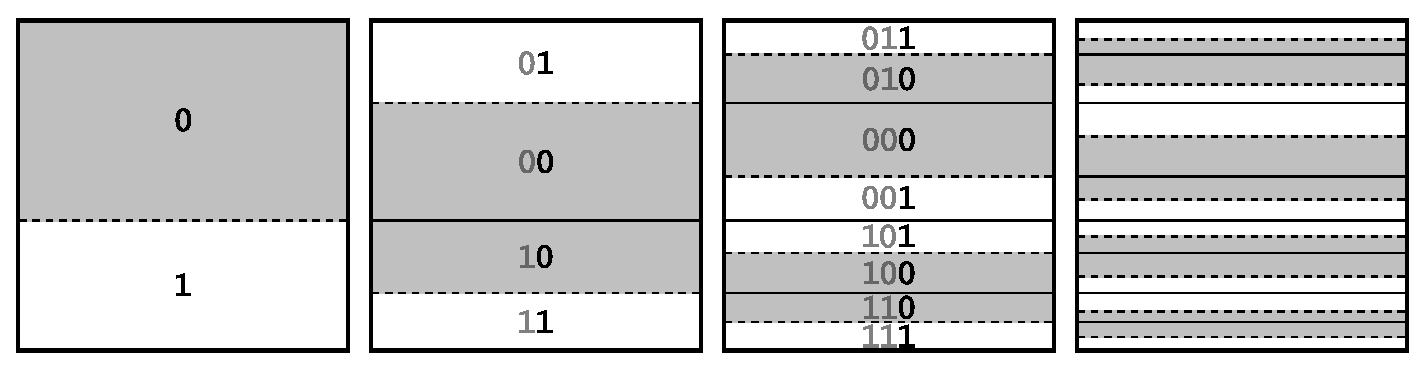
\includegraphics[width=\textwidth]{1dpart.eps}
\caption{\label{fig:1dpart}%
  First four levels of 1-Dimensional Partitioning. Dashed lines show the
  divisions performed in each step; solid lines indicate regions delimited in
  previous steps (there are no border conflicts between spots separated by
  solid lines). Masked (shaded) regions are labeled ``0'',
  unmasked (white) regions are labeled ``1''. This labeling forms
  a Gray code (shown in the first three steps only).}
\end{figure}


The next assignments of subsets to the upper or lower band of their regions
are made in such a way that regions with the same ``state'' --- productive
(unmasked) or unproductive (masked) --- are joined as far as
possible, resulting in masks that consist of alternating layers of masked and
unmasked spots. This process is illustrated in Fig.~\ref{fig:1dpart}, where at
each step~$t$, a band is labeled ``0'' when its embeddings are unproductive,
and ``1'' when its embeddings are productive. The resulting binary numbers
from top to bottom form a Gray code, i.e., two successive numbers differ in
only one bit.

The Gray code highlights an interesting property of 1-D Partitioning.
After $d$~levels of partitionings (based on steps $1$ to $d$), the
embeddings of any two immediate neighbors differ among the first
$d$~steps in at most one step.  As a result, masks $M_1 \dots M_d$
exhibit a layered structure that effectively reduces border conflicts.

Unfortunately, the Gray code is disrupted as soon as a region cannot be divided
(because all probes of that region are, for instance, masked at a particular
step). This will certainly happen as several binary numbers are unlikely to be
substrings of embeddings (think of, for example, a long run of zeros).

Moreover, 1-D Partitioning can optimize only a limited number of masks
because the sub-regions soon become too narrow to be further divided. The
maximum \emph{partitioning depth} $d_{max}$ is primarily limited by the number
of rows in the chip. In practice, since regions are likely to be unevenly
divided, $d_{max}$ varies between regions. The algorithm can also be configured
to stop partitioning a region once its dimensions drop below a given threshold.

1-D Partitioning is easier to implement if the partitionings always produce
rectangular regions (i.e., splitting a row between two regions is not allowed).
In order to force an exact division of a region, however, it might be necessary
to move a few probes from one subset of probes to the other one.

For example, imagine that a chip with $|\mathcal{P}| = 900$ probes, $n_r = 30$
rows and $n_c = 30$ columns is to be partitioned based on the state of the
embeddings at the first synthesis step, resulting in sub-sets $\mathcal{P}_0$
and $\mathcal{P}_1$ with, say, 638 and 262 probes, respectively. The chip must
thus be divided into two sub-regions, the upper one containing $[30 \cdot
638/900]=21$ rows and the lower one with $[30 \cdot 262/900]=9$ rows ($[x]$ is
$x$ rounded to the nearest integer). The problem is that the upper region then
contains $21 \cdot 30 = 630$ spots but it has to accommodate 638 probes,
whereas the lower region contains $9 \cdot 30 = 270$ spots but only 262
probes. The solution is to (arbitrarily) move 8 probes from $\mathcal{P}_0$ to
$\mathcal{P}_1$, which, results in some imperfections in the layers
of the corresponding mask (a few masked spots in a region of unmasked spots,
for instance).

\section{2-Dimensional Partitioning}
\label{sec:part_2d}

%%%
\begin{figure}\centering
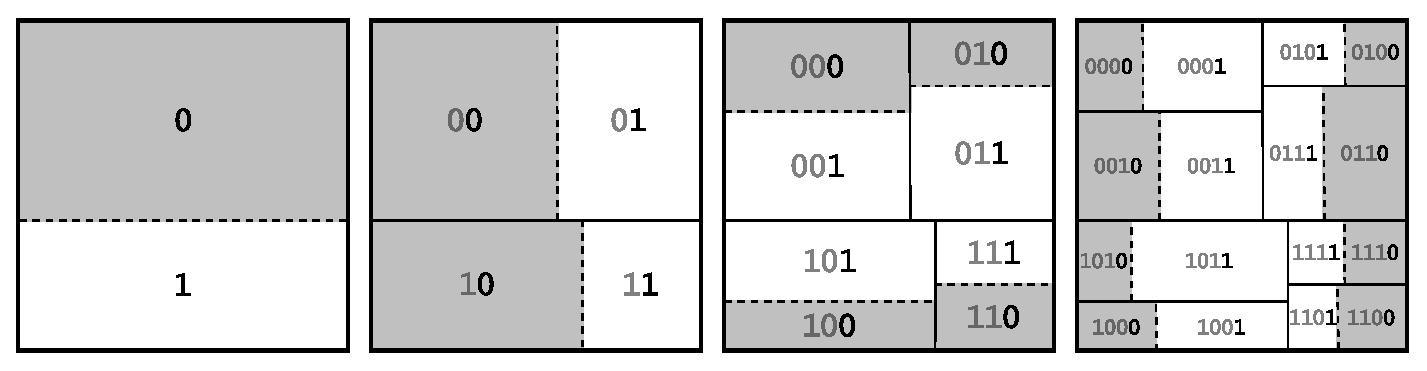
\includegraphics[width=\textwidth]{2dpart.eps}
\caption{\label{fig:2dpart}%
  First four levels of 2-Dimensional Partitioning. Dashed lines show
  the divisions performed in each step; solid lines indicate regions
  delimited in previous steps. Masked regions are labeled with ``0'',
  unmasked regions with ``1''; this labeling forms an approximation to
  a two-dimensional Gray code.}%
\end{figure}
%%%

The 2-Dimensional Partitioning algorithm extends the idea of 1-D
Partitioning to two dimensions, with the potential of optimizing twice
as many masks. The algorithm is similar: $\mathcal{P}$ is divided into
subsets based on the state of the embeddings at a particular
synthesis step. The difference is that 2-D Partitioning alternates
horizontal and vertical divisions of regions, and that the assignments
of probes to regions obey a two-dimensional Gray code
(Fig.~\ref{fig:2dpart}).

In a 2-D Gray code, two neighboring numbers differ in at most one
bit.  Thus, regions whose embeddings are at the same state (productive or
unproductive) are joined as far as possible.

If regions were always equally divided, 2-D Partitioning would have
the same property as 1-D Partitioning: After $d$~levels of
partitionings (based on steps $1$ to $d$), the embeddings of any two
immediate neighbors would differ among the first $d$ steps in at most
one step. However, this is not always the case since 2-D Partitioning
is likely to create regions with different dimensions, forcing some
regions to share a border with more than its four natural neighbors
(for example, region ``1100'' in Fig.~\ref{fig:2dpart} borders with
``0101'' and ``1111'').

So far we have described both 1-D and 2-D Partitionings using the
state of the first $d$ synthesis steps to divide the set of probes.
The result of this approach is that, while the first masks are
optimized, the remaining masks are left with high levels of border
conflicts; we call this a \emph{left-most mask optimization}.

However, a defect in the middle of the probe is more harmful than in
its extremities, so it is more important to optimize the central masks,
which synthesize the middle bases. Thus we
partition the chip based on the following sequence
of synthesis steps, assuming that $T$ is even and $d$ is odd: $T/2,
(T/2)\pm 1, (T/2)\pm 2, \dots, (T/2)\pm\lfloor d/2\rfloor$; we call
this a \emph{centered mask optimization}.

For left-most optimization, it makes sense to embed the probes in a
left-most fashion in order to reduce conflicts in the last masks
(which are not optimized by the partitioning); the left-most
embeddings reduce the number of unmasked spots in the last steps,
resulting in masks that largely consist of masked spots. Similarly,
centered mask optimization produces better results with \emph{centered
  embeddings}. A centered embedding is constructed by shifting a
left-most embedding to the right so that the number of masked steps to
the left of the first productive step approximately equals the number
of masked steps to the right of the last productive step.

%%%
\begin{figure}\centering
%%
\begin{picture}(335,150)\footnotesize{
  \put(0,0){\makebox(335,150){
    %GNUPLOT: LaTeX picture with Postscript
    \begin{picture}(0,0)%
    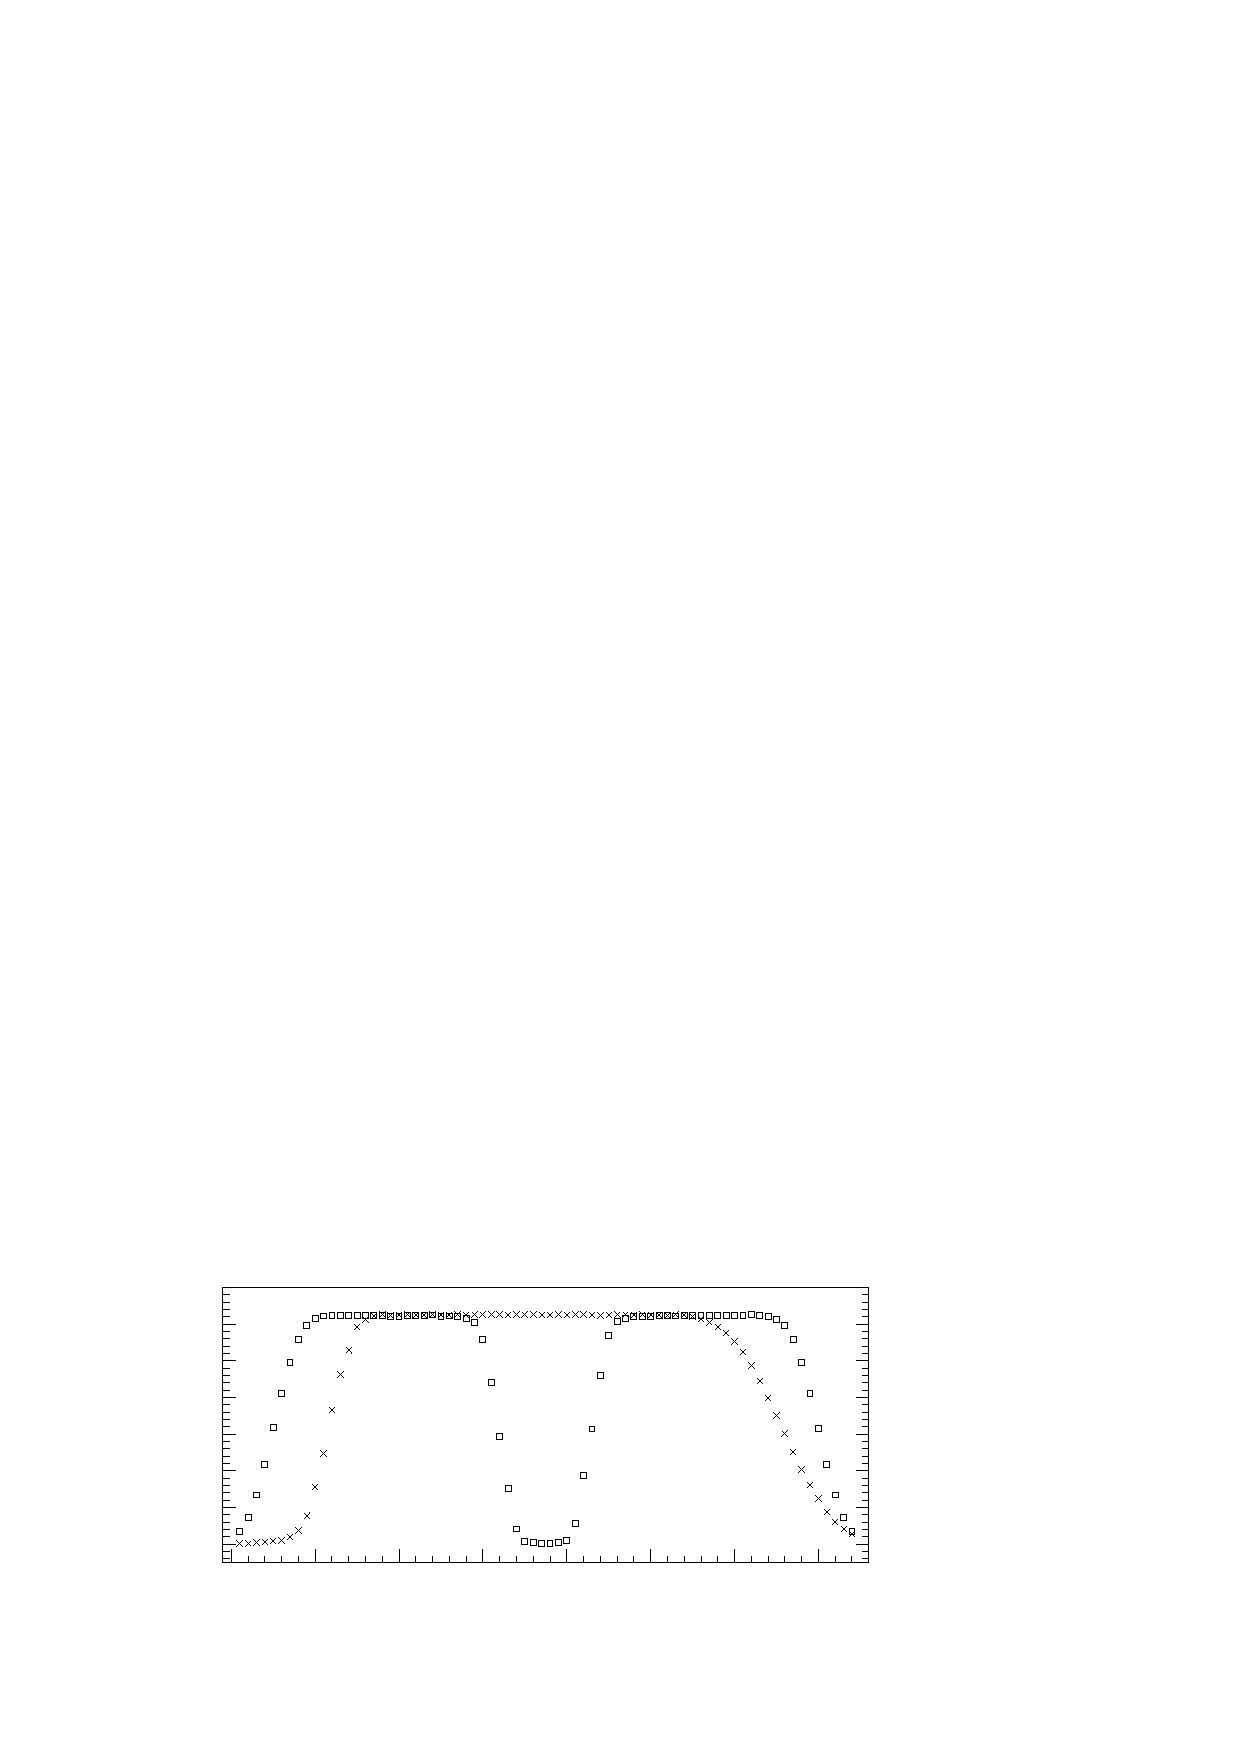
\includegraphics{2dpart_bl/2dpart_bl}%
    \end{picture}%
    \begingroup
    \setlength{\unitlength}{0.0200bp}%
    \begin{picture}(18000,8100)(0,0)%
    \put(1500,1440){\makebox(0,0)[r]{\strut{} 0}}%
    \put(1500,2320){\makebox(0,0)[r]{\strut{} 0.1}}%
    \put(1500,3200){\makebox(0,0)[r]{\strut{} 0.2}}%
    \put(1500,4080){\makebox(0,0)[r]{\strut{} 0.3}}%
    \put(1500,4960){\makebox(0,0)[r]{\strut{} 0.4}}%
    \put(1500,5840){\makebox(0,0)[r]{\strut{} 0.5}}%
    \put(1500,6720){\makebox(0,0)[r]{\strut{} 0.6}}%
    \put(1500,7600){\makebox(0,0)[r]{\strut{} 0.7}}%
    \put(1951,500){\makebox(0,0){\strut{} 0}}%
    \put(3964,500){\makebox(0,0){\strut{} 10}}%
    \put(5977,500){\makebox(0,0){\strut{} 20}}%
    \put(7990,500){\makebox(0,0){\strut{} 30}}%
    \put(10003,500){\makebox(0,0){\strut{} 40}}%
    \put(12016,500){\makebox(0,0){\strut{} 50}}%
    \put(14029,500){\makebox(0,0){\strut{} 60}}%
    \put(16042,500){\makebox(0,0){\strut{} 70}}%
    \end{picture}%
    \endgroup
  }}
}\end{picture}
%%
%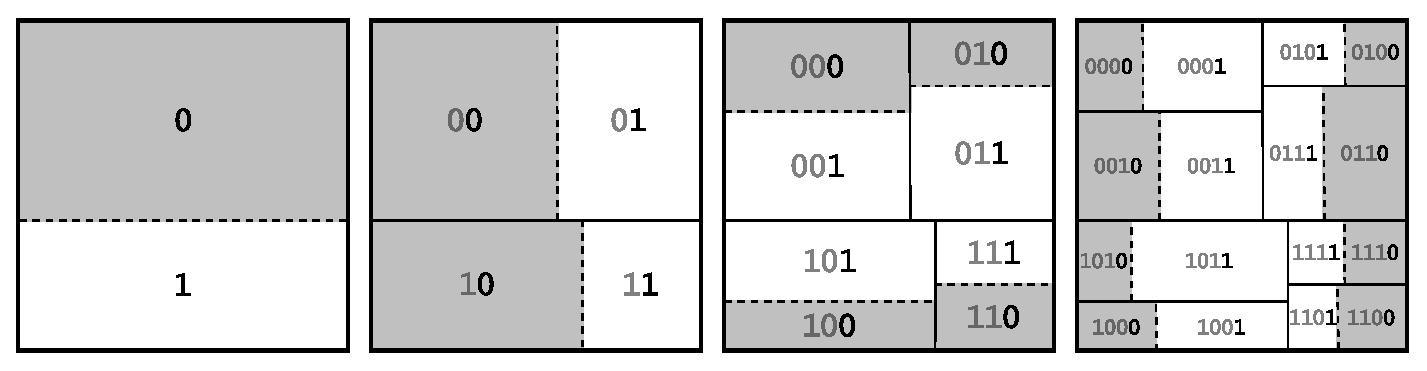
\includegraphics[width=\textwidth]{2dpart.eps}
\caption{\label{fig:2dpart_bl}%
  Normalized border length (on the y-axis) per masking step (on the x-axis) of
  a layout produced by 2-Dimensional Partitioning for a $1\,000 \times 1\,000$
  chip with random probe sequences (embedded in the standard 74-step Affymetrix
  deposition sequence). Partitioning stops when a region becomes smaller than
  $64 \times 64$; Row-Epitaxial is used for the placement. ({\tiny $\times$})
  Left-most mask optimization with left-most embeddings; ({\tiny $\Box$})
  centered mask optimization with centered embeddings.}
\end{figure}
%%%

Fig.~\ref{fig:2dpart_bl} shows the results of 2-D Partitioning on a
$1\,000\times 1\,000$ chip with both optimizations. For left-most mask
optimization, we obtain a normalized border length of 33.89 (up to
approximately 0.6 per step). For centered mask optimization, the normalized
border length improves slightly to 33.59. The average conflict index (not
shown in the figure) for left-most mask optimization is 571.8; for centered
mask optimization, it improves considerably to 383.5 because of the higher
weight of the middle bases.


\section{Centroid-based Quadrisection}
\label{sec:part_cq}

\begin{figure}\centering
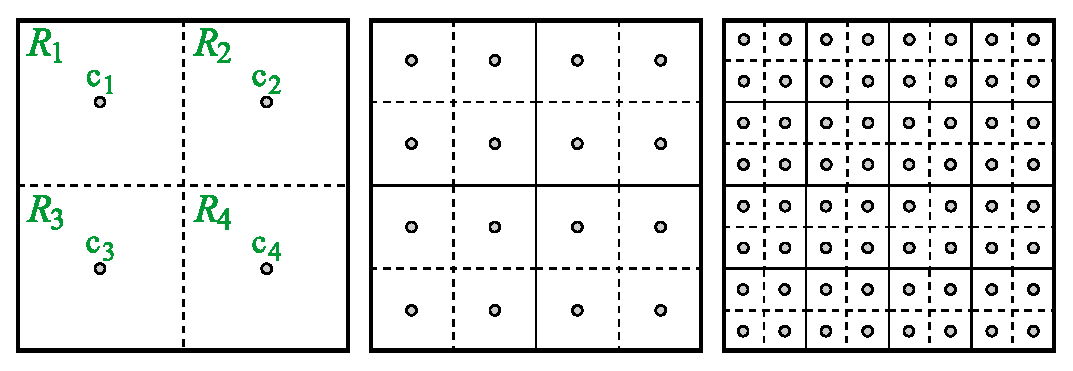
\includegraphics[width=\textwidth]{quadrisect.eps}
\caption{\label{fig:quadrisect}%
  First three levels of Centroid-base Quadrisection Partitioning. Dashed lines
  show the divisions performed in each step; solid lines indicate regions
  delimited in previous steps. The centroids of each partition $R_1 \dots R_4$
  are represented by small circles (labeled with $q_1 \dots q_4$ in the first
  step).}
\end{figure}

Centroid-based Quadrisection or CQ \citep{Kahng2003a} employs a
different criterion for dividing the set of probes and a different
approach for partitioning. At each iteration, a region $R$ is
quadrisectioned into $R_1$, $R_2$, $R_3$, and $R_4$. Each sub-region
$R_i$ is associated with a selected probe $p_{c_i}\in \mathcal{P}$,
called \emph{centroid}, that is used to guide the assignment of the
remaining probes to the sub-regions.

A centroid is a representative of its region; it should symbolize the
``average embedding'' in that region. The remaining probes $p_k \in
\mathcal{P} \setminus \{p_{c_1},p_{c_2},p_{c_3},p_{c_4}\}$ are
compared to each centroid and assigned to the sub-region $R_i$ whose
centroid's embedding $\eps_{c_i}$ has minimum $H(k,c_i)$, where
$H(k,k')$ is the Hamming distance between the embeddings $\eps_k$ of
$p_k$ and $\eps_{k'}$ of $p_{k'}$ (i.e., the number of steps in which
$\eps_k$ and $\eps_{k'}$ differ).

In order to improve the clustering of similar probes, the four
centroids should be very different from each other. The following
heuristic is used: First, a probe index $c_1$ is randomly selected
from $\{1,\dots,|\mathcal{P}|\}$.  Then, a probe index $c_2\neq c_1$
maximizing $H(c_2,c_1)$ is selected.  Similarly, $c_3$ maximizing
$H(c_3,c_1) + H(c_3,c_2)$ and $c_4$ maximizing $H(c_4,c_1) +
H(c_4,c_2) + H(c_4,c_3)$ are selected.  The assignment of centroids to
the quadrisections of the chip is arbitrary.

In order to recover from a possibly bad choice of centroids, one can
use a ``multi-start heuristic'', running the centroid selection
procedure several times (using different ``seeds'' for $c_1$), and
keeping those that lead to the best partitioning (partitioning quality
is measured by the sum of Hamming distances of probe embeddings to
their corresponding centroid embeddings).

The partitioning continues recursively until a pre-defined depth has been
reached.

CQ was developed for border length minimization, but can be adapted
for conflict index minimization by using the \emph{conflict index
  distance} $C(k,k')$ instead of the Hamming distance $H(k,k')$
between the embeddings $\eps_k$ and $\eps_{k'}$,
%%
\begin{equation}
\label{eq:ci_dist}
C(k,k') := \sum_{t=1}^{T}
  \Bigl(
    \Ind{\eps_{k,t}=0 \text{ and } \eps_{k',t}=1}
    \cdot \omega(\eps_{k},t)
    +
    \Ind{\eps_{k',t}=0 \text{ and } \eps_{k,t}=1}
    \cdot \omega(\eps_{k'},t)
  \Bigr).
\end{equation}
%%
It can be interpreted as the sum of the conflict indices resulting
from placing probes $p_k$ and $p_{k'}$ at hypothetical neighboring
spots, ignoring the distance between these spots and the conflicts
generated by other neighbors.


\section{Pivot Partitioning: Merging partitioning and re-embedding}
\label{sec:part_pp}

Pivot Partitioning or PP \citep{Carvalho2006} is, to a certain extent,
similar to CQ: Sub-regions are recursively associated with special
probes $p_{c_i}$, here called \emph{pivots} instead of centroids, that
are used to guide the assignment of the other probes to the
sub-regions.  The main differences between PP and CQ are as follows.

Instead of quadrisectioning the chip, PP creates sub-regions by
alternating horizontal and vertical divisions (like 2-D Partitioning).
The advantage is that regions are divided proportionally to the size
of each subset of probes, so they are not required to have the same
size. Furthermore, for each partitioning level, only two pivots need
to be selected.

Another distinction is motivated by the fact that different probes
have different numbers of embeddings, ranging from a single one to
several millions.  Probes with more embeddings can more easily adapt
to the other probes, that is, they are more likely to have an
embedding with fewer conflicts to fill a particular spot than a probe
that has only a limited number of embeddings. For this reason, PP uses
probes with a single embedding (or few embeddings) as pivots, and
chooses the other probes' embeddings and region assignments accordingly.

Indeed, the most important feature of PP is the simultaneous embedding and
assignment of probes to sub-regions. Let $M(k,c_i)$ denote the minimum
conflict index distance $C(k,c_i)$, as defined in~(\ref{eq:ci_dist}), over all
embeddings of $p_k$; we call it the \emph{minimum conflict index distance}
between probes $p_k$ and $p_{c_i}$. It can be efficiently computed with a
variant of the OSPE algorithm that ignores the location of the probes and the
distance-dependent weights $\gamma$. Now, a non-pivot probe $p_k$ is assigned
to the region $R_i$ whose pivot $p_{c_i}$ has minimum $M(k,q_i)$ over $i=1,2$.
Pivot Partitioning continues recursively up to a pre-defined depth. Finally,
each probe is embedded to minimize conflicts with its assigned pivot.

%%%%%%%%%%%%%%%%%%%%%%%%%%%%%%%%%%%%%%%%%%%%%%%%%%%%%%%%%%%%%%%%%%%%%%%%%%%%%%%%
\chapter{Merging Placement and Re-embedding}
\label{ch:merge}
%%%%%%%%%%%%%%%%%%%%%%%%%%%%%%%%%%%%%%%%%%%%%%%%%%%%%%%%%%%%%%%%%%%%%%%%%%%%%%%%

In the previous chapters we have reviewed several algorithms that deal with the
Microarray Layout Problem in the traditional way: partitioning, placement and
re-embedding. The problem with the ``place and re-embed'' approach is that once
the placement is fixed, there is usually little freedom for optimization by
re-embedding the probes. Intuitively, better results should be obtained when the
placement and embedding phases are considered simultaneously instead of
separately. However, because of the generally high number of embeddings of each
single probe, it is not easy to design algorithms that efficiently use the
additional freedom and run reasonably fast in practice. In Chapter
\ref{ch:part}, we have shown how Pivot Partitioning successfully explored this
extra freedom to outperform previous partitioning algorithms.

In this chapter, we describe the first placement algorithm that simultaneously
places and re-embeds the probes. Our goal was to design an algorithm that is
similar to the Greedy placement algorithm (Section \ref{sec:placement_greedy}),
so that we can make a better assessment of the gains resulting from merging the
placement and re-embedding phases.

%%%%%%%%%%%%%%%%%%%%%%%%%%%%%%%%%%%%%%%%%%%%%%%%%%%%%%%%%%%%%%%%%%%%%%%%%%%%%%%%
\section{\Greedyplus}
\label{sec:merge_greedyplus}

\Greedyplus\ is similar to Greedy in many respects. Spots are filled in a greedy
fashion, sequentially, using a user-configurable $k$-threading pattern. For each
spot $s$, \Greedyplus\ looks at $Q$ probe candidates and chooses the one that
can be placed at $s$ with minimum cost. The main difference is that \Greedyplus\
considers all possible embeddings of a candidate $p$ instead of only $p$'s given
embedding. This is done by temporarily placing $p$ at the spot $s$ and using
OSPE (Section~\ref{sec:reembed_ospe}) to compute $p$'s optimal embedding with
respect to the already-filled neighbors of $s$. Naturally, OSPE can be used to
compute the optimal embedding with respect to border length or conflict index.

Compared to Greedy, \Greedyplus\ spends more time evaluating each probe
candidate $p$ for filling a spot $s$. While Greedy takes $O(T)$ time to compute
the conflict index or the border length resulting from placing $p$ at $s$,
\Greedyplus\ requires $O(\ell \cdot T)$ time since it uses OSPE (recall that
$\ell$ is the probe length and $T$ is the deposition sequence length). We must
therefore use lower numbers $Q$ of candidates per spot to achieve a running
time comparable to Greedy.

There are three observations that significantly reduce the time spent with OSPE
computations when several probe candidates are considered in succession for
filling the same spot. First, we note that the $U_t$ and $M_{i,t}$ costs of OSPE
(Equations \ref{eq:ospe_ucost} and \ref{eq:ospe_mcost}, respectively) need to be
computed only once for a given spot $s$ since they do not depend on the probe
placed at $s$ but rather on the probes placed at neighbors of $s$: $U_t$ depends
solely on the neighbors of $s$, whereas $M_{i,t}$ depends on the neighbors of
$s$ and on the number $i$ of bases probe $p$ already contains at synthesis step
$t$ (assumming that all probes have the same length $\ell$; $c$ and $\theta$ in
Equation \ref{eq:ospe_mcost} are constants).

Second, once we know that a probe candidate $p$ can be placed at the spot $s$
with minimum cost $\kappa$, we can stop the OSPE computation for another
candidate $p'$ as soon as all values in a row of OSPE's dynamic programming
matrix are greater than or equal to $\kappa$.

Finally, we note that if two probe sequences $p$ and $p'$ share a common prefix
of length $r$, the first $r + 1$ rows of OSPE's matrix $D$ will be identical.
Hence, if we have previously calculated the minimum cost of $p$, we can speed up
the calculation of the minimum cost of $p'$ by skipping the first $r + 1$ rows
of $D$. In order to fully exploit this fact, we must examine the probes in
lexicographical order so that we maximize the length of the common prefix
between two consecutive probe candidates. For this reason, \Greedyplus\ uses the
same technique used by Greedy: Initially, the probe sequences are sorted
lexicographically and stored in a doubly-linked list. Once a probe $p$ is
selected to fill the current spot, it is removed from the list. For the next
spot to be filled, \Greedyplus\ looks at $Q$ probes in the list around $p$'s
former position, e.g., at $\lfloor Q/2 \rfloor$ probes to the left and at
$\lceil Q/2 \rceil$ probes to the right of $p$ (the list is traversed from left
to right).

%%%%%%%%%%%%%%%%%%%%%%%%%%%%%%%%%%%%%%%%%%%%%%%%%%%%%%%%%%%%%%%%%%%%%%%%%%%%%%%%
\section{Results}
\label{sec:merge_results}

\begin{table}[p!]\centering
\caption{\label{tab:greedyplus_nbl}
  Normalized border length (NBL) of layouts produced by \Greedyplus\ on random
  chips with varying number $Q$ of candidades per spot and amplitude of
  $k$-threading. Running times are reported in minutes.}
\footnotesize{
\begin{tabular}{crcrlcrlcr}
\vspace{1pt}
     &     & \multicolumn{2}{c}{$Q=500$} & & \multicolumn{2}{c}{$Q=1\,000$} & & \multicolumn{2}{c}{$Q=2\,000$} \\ \cline{3-4} \cline{6-7} \cline{9-10}
\vspace{1pt}
Dim. & $k$ & NBL & Time & & NBL & Time & & NBL & Time \\
\hline
$300\times 300$ &  0 &      17.9356  &  5.4 &  &      17.7136  & 10.6 &  &      17.5460  &  20.6 \\
                &  1 &      18.0922  &  5.4 &  &      17.8988  & 10.5 &  &      17.7501  &  20.4 \\
                &  2 &      17.9886  &  5.4 &  &      17.7905  & 10.5 &  &      17.6342  &  20.5 \\
                &  3 &      17.9339  &  5.7 &  &      17.7406  & 10.5 &  &      17.5799  &  20.5 \\
                &  4 &      17.8978  &  5.7 &  &      17.7155  & 11.1 &  &      17.5506  &  20.5 \\
                &  5 &      17.8862  &  5.7 &  &      17.7013  & 10.6 &  &      17.5359  &  20.5 \\
                &  6 &      17.8749  &  5.4 &  &      17.6908  & 10.6 &  &      17.5225  &  20.5 \\
                &  7 &      17.8641  &  5.5 &  &      17.6807  & 10.6 &  &      17.5223  &  20.6 \\
                &  8 &      17.8605  &  5.4 &  &      17.6711  & 10.6 &  &      17.5141  &  20.6 \\
                &  9 &      17.8519  &  5.4 &  &      17.6685  & 10.6 &  &      17.5083  &  20.6 \\
                & 10 &      17.8518  &  5.4 &  &      17.6657  & 10.6 &  &      17.5067  &  20.6 \\
                & 11 &      17.8427  &  5.5 &  &      17.6705  & 10.6 &  &      17.5066  &  20.6 \\
                & 12 &      17.8431  &  5.4 &  &      17.6643  & 10.6 &  &      17.5070  &  20.6 \\
                & 13 &      17.8455  &  5.4 &  & {\bf 17.6628} & 10.6 &  & {\bf 17.5021} &  20.6 \\
                & 14 & {\bf 17.8423} &  5.4 &  &      17.6629  & 10.6 &  &      17.5053  &  20.5 \\
\hline
$500\times 500$ &  0 &      17.3240  & 14.9 &  &      17.0576  & 29.1 &  &      16.8707  &  57.0 \\
                &  1 &      17.4648  & 14.8 &  &      17.2483  & 28.9 &  &      17.0761  &  56.5 \\
                &  2 &      17.3372  & 14.9 &  &      17.1318  & 29.0 &  &      16.9650  &  56.4 \\
                &  3 &      17.2732  & 14.9 &  &      17.0785  & 29.0 &  &      16.9135  &  56.5 \\
                &  4 &      17.2371  & 14.9 &  &      17.0436  & 29.0 &  &      16.8855  &  56.8 \\
                &  5 &      17.2143  & 14.9 &  &      17.0264  & 29.3 &  &      16.8676  &  57.2 \\
                &  6 &      17.1990  & 15.0 &  &      17.0141  & 29.3 &  &      16.8557  &  57.2 \\
                &  7 &      17.1812  & 15.0 &  &      17.0049  & 29.3 &  &      16.8420  &  57.2 \\
                &  8 &      17.1774  & 15.0 &  &      16.9965  & 29.3 &  &      16.8398  &  57.0 \\
                &  9 &      17.1704  & 15.0 &  &      16.9921  & 29.4 &  &      16.8346  &  57.3 \\
                & 10 &      17.1666  & 15.8 &  &      16.9876  & 29.2 &  &      16.8332  &  59.7 \\
                & 11 &      17.1629  & 15.0 &  &      16.9814  & 29.1 &  &      16.8294  &  56.8 \\
                & 12 &      17.1594  & 14.9 &  &      16.9821  & 29.3 &  &      16.8280  &  56.7 \\
                & 13 &      17.1549  & 15.8 &  &      16.9767  & 29.1 &  & {\bf 16.8240} &  56.8 \\
                & 14 & {\bf 17.1503} & 14.9 &  & {\bf 16.9737} & 29.1 &  &      16.8261  &  56.8 \\
\hline
$800\times 800$ &  0 &      16.7983  & 38.0 &  &      16.4944  & 73.8 &  &      16.2640  & 144.4 \\
                &  1 &      16.8849  & 37.7 &  &      16.6615  & 73.3 &  &      16.4780  & 143.3 \\
                &  2 &      16.7420  & 37.8 &  &      16.5377  & 73.5 &  &      16.3626  & 143.6 \\
                &  3 &      16.6693  & 37.9 &  &      16.4775  & 73.9 &  &      16.3070  & 143.9 \\
                &  4 &      16.6266  & 38.0 &  &      16.4375  & 73.8 &  &      16.2707  & 144.2 \\
                &  5 &      16.5938  & 38.1 &  &      16.4096  & 74.2 &  &      16.2497  & 145.1 \\
                &  6 &      16.5700  & 38.2 &  &      16.3919  & 74.3 &  &      16.2334  & 145.2 \\
                &  7 &      16.5543  & 38.2 &  &      16.3801  & 74.6 &  &      16.2237  & 145.2 \\
                &  8 &      16.5435  & 38.1 &  &      16.3691  & 74.5 &  &      16.2171  & 145.3 \\
                &  9 &      16.5379  & 38.2 &  &      16.3646  & 74.7 &  &      16.2115  & 145.8 \\
                & 10 &      16.5297  & 38.0 &  &      16.3586  & 74.0 &  &      16.2094  & 144.5 \\
                & 11 &      16.5229  & 38.0 &  &      16.3539  & 74.0 &  &      16.2039  & 144.5 \\
                & 12 &      16.5210  & 38.2 &  &      16.3518  & 74.1 &  &      16.2022  & 144.6 \\
                & 13 &      16.5194  & 38.1 &  &      16.3474  & 74.1 &  &      16.1971  & 144.7 \\
                & 14 & {\bf 16.5118} & 38.0 &  & {\bf 16.3456} & 74.1 &  & {\bf 16.1968} & 144.8 \\
\hline
\end{tabular}}
\end{table}

\begin{table}[t]\centering
\caption{\label{tab:greedyplus_aci}
  Average conflict index (ACI) of layouts produced by \Greedyplus\ on random
  chips with varying number $Q$ of candidades per spot and $k$-threading's
  amplitude. Running times are reported in minutes.}
\footnotesize{
\begin{tabular}{crcrlcrlcr}
\vspace{1pt}
     &     & \multicolumn{2}{c}{$Q=500$} & & \multicolumn{2}{c}{$Q=1\,000$} & & \multicolumn{2}{c}{$Q=2\,000$} \\ \cline{3-4} \cline{6-7} \cline{9-10}
\vspace{1pt}
Dim. & $k$ & ACI & Time & & ACI & Time & & ACI & Time \\
\hline
$300\times 300$ &  0 & {\bf 462.3882} &  5.8 &  & {\bf 443.3786} & 10.5 &  & {\bf 425.9132} &  19.8 \\
                &  1 &      468.6485  &  5.8 &  &      449.1931  & 10.6 &  &      431.1021  &  19.9 \\
                &  2 &      472.3753  &  5.8 &  &      452.5054  & 10.6 &  &      434.1209  &  19.9 \\
                &  3 &      474.3210  &  5.8 &  &      454.6870  & 10.6 &  &      436.2880  &  20.0 \\
                &  4 &      474.2031  &  5.8 &  &      454.6782  & 10.6 &  &      436.2529  &  19.9 \\
\hline
$500\times 500$ &  0 & {\bf 457.3329} & 15.8 &  & {\bf 437.3920} & 28.8 &  & {\bf 419.2114} &  54.2 \\
                &  1 &      463.6259  & 16.0 &  &      443.7018  & 30.4 &  &      424.5009  &  54.7 \\
                &  2 &      467.3461  & 15.9 &  &      447.5021  & 29.0 &  &      428.3882  &  54.8 \\
                &  3 &      469.2554  & 16.6 &  &      449.4136  & 29.1 &  &      430.4992  &  55.0 \\
                &  4 &      468.9371  & 16.0 &  &      449.5197  & 29.1 &  &      430.4662  &  58.0 \\
\hline
$800\times 800$ &  0 & {\bf 451.8074} & 40.0 &  & {\bf 431.8977} & 73.0 &  & {\bf 413.3451} & 144.3 \\
                &  1 &      458.1598  & 40.3 &  &      437.8440  & 73.5 &  &      418.9562  & 138.4 \\
                &  2 &      461.6418  & 40.3 &  &      441.6484  & 73.3 &  &      423.0075  & 145.9 \\
                &  3 &      463.5349  & 40.3 &  &      443.7868  & 73.6 &  &      425.2302  & 138.9 \\
                &  4 &      463.1225  & 40.3 &  &      443.7802  & 73.7 &  &      425.3695  & 139.0 \\
\hline
\end{tabular}}
\end{table}

We first examine how the amplitude of the $k$-threading and the number $Q$ of
candidates per spot affect the results of \Greedyplus. In the case of BLM (Table
\ref{tab:greedyplus_nbl}), the best results were always achieved with
surprisingly high values of $k$ (this is in contrast to Greedy, which always
produced the best results with $k=0$). The reason is not yet clear, especially
because only conflicts between adjacent spots count in the border length model.
It should also be noted that for a sufficiently large value of $k$, a
``row-wise'' $k$-threading can be seen as a ``column-wise'' 0-threading.

With BLM, increasing the amplitude from $k=0$ to $k=1$ always worsened the
results. Increasing it further, however, improved the layouts and eventually
resulted in less conflicts than with $k=0$ up to a point when it started to make
little difference. The greatest difference between the worse and the best
layouts due to the amplitude $k$ was at most $2.26\%$ (from $16.5118$ with
$k=14$ to $16.8849$ with $k=1$ on $800\times 800$ chips and $Q=500$). In case of
CIM (Table \ref{tab:greedyplus_aci}), the best results were always achieved with
$k=0$, and increasing it up to $k=3$ always resulted in more conflicts, although
increasing it to $k=4$ often resulted in slightly better layouts than with
$k=3$.

In both cases, doubling the number $Q$ of candidates per spot roughly doubled
the running time. In contrast with Greedy, \Greedyplus\ requires approximately
the same time with CIM and BLM, sometimes being even slightly faster with the
former. This can be explained as follows. The major difference the quality
measure makes for OSPE, in terms of running time, is when the $U_t$ and
$M_{i,t}$ costs of OSPE are computed. While for BLM at most four neighbors of a
spot $s$ need to be examined, for CIM we must look at up to 48 neighbors of $s$.
However, since the $U_t$ and $M_{i,t}$ costs are computed only once for a spot
$s$ and are reused for each of the $Q$ candidate probes, the greater the number
$Q$, the less impact the quality measure makes in total running time. The fact
that \Greedyplus\ is sometimes slightly faster with CIM than with BLM could be
because, with the former, it more quickly finds a probe candidate with a low
minimum cost $\kappa$ that allows it to stop computing the cost of other
candidates sooner (when all entries in a row of OSPE's matrix are greater than
$\kappa$).

\begin{table}[t!]\centering
\caption{\label{tab:greedycomp_bl}
  Normalized border length (NBL) of layouts produced by Greedy and \Greedyplus\
  on random chips with the number $Q$ of candidades per spot of \Greedyplus\ set
  in such a way that it does not exceed the time spent by Greedy. Total time
  including placement and re-embedding is reported in minutes. Both algorithms
  use $0$-threading and are followed by two passes of re-embedding optimization
  with Sequential. The relative difference in NBL and time between the two
  approaches is shown in percentage.}
\footnotesize{
\begin{tabular}{crrrlrrrlrr}
\vspace{1pt}
                & \multicolumn{3}{c}{Greedy and Sequential} & & \multicolumn{3}{c}{\Greedyplus\ and Sequential} & & \multicolumn{2}{c}{Relative} \\ \cline{2-4} \cline{6-8} \cline{10-11}
\vspace{1pt}
Dim.            & Q       & NBL     & Time  & & Q      & NBL     & Time & & NBL       & Time \\
\hline
$300\times 300$ & 10\,000 & 18.0900 &   6.2 & &    300 & {\bf 17.9807} &  4.2 & & $-0.60\%$ & $-31.21\%$ \\
                & 20\,000 & 17.9725 &  12.1 & &    700 & {\bf 17.6746} &  9.2 & & $-1.66\%$ & $-23.85\%$ \\
\hline
$500\times 500$ & 10\,000 & 17.3809 &  20.8 & &    450 & {\bf 17.2216} & 16.0 & & $-0.92\%$ & $-23.30\%$ \\
                & 20\,000 & 17.2779 &  41.9 & &    950 & {\bf 16.9382} & 30.4 & & $-1.97\%$ & $-27.42\%$ \\
\hline
$800\times 800$ & 10\,000 & 16.7143 &  57.9 & &    500 & {\bf 16.6549} & 41.7 & & $-0.36\%$ & $-28.00\%$ \\
                & 20\,000 & 16.6259 & 121.6 & & 1\,130 & {\bf 16.3175} & 97.7 & & $-1.85\%$ & $-19.68\%$ \\
\hline
\end{tabular}}
\end{table}

\begin{table}[t!]\centering
\caption{\label{tab:greedycomp_ci}
  Average conflict index (ACI) of layouts produced by Greedy and \Greedyplus\
  (with $0$-threading) on random chips in approximately the same amount of time
  (total time in minutes including two passes of Sequential re-embedding
  optimization). The relative difference in ACI between the two approaches is
  shown in percentage.}
\footnotesize{
\begin{tabular}{crcrlrcrlr}
\vspace{1pt}
                & \multicolumn{3}{c}{Greedy and Sequential} & & \multicolumn{3}{c}{\Greedyplus\ and Sequential}   \\ \cline{2-4} \cline{6-8}
\vspace{1pt}
Dim.            & Q        & ACI            & Time     & & Q       & ACI            & Time      & & Relative \\
\hline
$300\times 300$ &  10\,000 & {\bf 423.1330} &     13.9 & &  1\,070 &      438.4015  &     14.0 &  & $+3.61\%$ \\
                &  20\,000 & {\bf 412.5536} &     24.1 & &  2\,180 &      420.8863  &     24.2 &  & $+2.02\%$ \\
                &  80\,000 &      402.4365  &     54.3 & &  5\,500 & {\bf 401.7005} &     54.0 &  & $-0.18\%$ \\
\hline
$500\times 500$ &  10\,000 & {\bf 412.5468} &     43.2 & &  1\,225 &      428.5082  &     43.7 &  & $+3.87\%$ \\
                &  20\,000 & {\bf 398.6096} &     77.0 & &  2\,580 &      409.6446  &     76.9 &  & $+2.77\%$ \\
                & 140\,000 &      375.5428  &    352.2 & & 13\,500 & {\bf 374.9914} &    351.9 &  & $-0.15\%$ \\
\hline
$800\times 800$ &  10\,000 & {\bf 405.3133} &    113.9 & &  1\,315 &      421.2380  &    113.7 &  & $+3.93\%$ \\
                &  20\,000 & {\bf 389.3929} &    207.9 & &  2\,790 &      401.7969  &    208.5 &  & $+3.19\%$ \\
                & 300\,000 &      350.8412  & 2\,056.7 & & 32\,000 & {\bf 350.6951} & 2\,050.8 &  & $-0.04\%$ \\
\hline
\end{tabular}}
\end{table}

We now compare the results obtained by Greedy and \Greedyplus\ when both
algorithms are given the same amount of time (the parameter $Q$ is chosen
differently for both algorithms so that the running time is approximately
comparable). To be fair, since Greedy is a traditional placement algorithm that
does not change the embeddings of the probes, we need to compare the layouts
obtained by both algorithms after a re-embedding phase. For this task we use the
Sequential algorithm (Section \ref{sec:reembed_sequential}) performing two
passes of re-embedding optimization. For this experiment we use probes of length
$\ell=25$ left-most embedded in the standard Affymetrix deposition sequence.

Table \ref{tab:greedycomp_bl} compares both algorithms in terms of border length
minimization. In all cases, \Greedyplus\ produced better layouts than Greedy in
the same amount of time (or less) while looking at fewer probe candidates. For
instance, on $800\times 800$ chips \Greedyplus\ with $Q=1\,130$ produced layouts
with $1.85\%$ less border conflicts than Greedy with $Q=20\,000$ in $19.68\%$
less time, on average.

In terms of CIM (Table \ref{tab:greedycomp_ci}), Greedy is not so easily
outperformed by \Greedyplus. With $Q=10\,000$ and $Q=20\,000$ Greedy produced
better layouts than \Greedyplus\ in approximately the same time. For instance,
on $800\times 800$ chips, \Greedyplus\ with $Q=2\,790$ produced layouts with
$3.19\%$ more conflicts than Greedy with $Q=20\,000$. However, \Greedyplus\ has
an advantage over Greedy since it needs to examine less candidates to achieve
similar results and, for sufficiently large values of $Q$, it is usually
possible to achieve better results with \Greedyplus\ in the same amount of time.
For instance, on $300\times 300$ chips, \Greedyplus\ with $Q=13\,500$ produced
layouts with only $0.18\%$ less conflicts than Greedy with $Q=80\,000$. After
this point, however, the difference in ACI between Greedy and \Greedyplus\ tends
to increase (data not shown). We also observed that the larger the chip, the
less advantage \Greedyplus\ has over Greedy. On $500\times 500$ chips,
\Greedyplus\ starts to outperform Greedy when $Q=13\,500$ (with running times in
the order of 6 hours), approximately, and on $800\times 800$ chips around
$Q=32\,000$ (with more than 34 hours of running time per array).

\begin{table}[t!]\centering
\caption{\label{tab:gplus_reptx}
  Normalized border length (NBL) of layouts produced by Row-Epitaxial and
  \Greedyplus\ (both with $0$-threading) on random chips in approximately the
  same amount of time. (total time in minutes including two passes of Sequential
  re-embedding optimization). The relative difference in NBL and time between
  the two approaches is shown in percentage.}
\footnotesize{
\begin{tabular}{crrrlrrrlrr}
\vspace{1pt}
                & \multicolumn{3}{c}{Row-Epitaxial and Sequential} & & \multicolumn{3}{c}{\Greedyplus\ and Sequential} & & \multicolumn{2}{c}{Relative} \\ \cline{2-4} \cline{6-8} \cline{10-11}
\vspace{1pt}
Dim.            & Q       & NBL     &  Time & & Q      & NBL     & Time & & NBL       & Time \\
\hline
$300\times 300$ & 10\,000 & 18.0524 &   4.3 & &    300 & {\bf 17.9807} &  4.2 & & $-0.40\%$ &  $-1.24\%$ \\
                & 20\,000 & 17.9430 &   9.5 & &    700 & {\bf 17.6746} &  9.2 & & $-1.50\%$ &  $-2.85\%$ \\
\hline
$500\times 500$ & 10\,000 & 17.3584 &  16.0 & &    450 & {\bf 17.2216} & 16.0 & & $-0.79\%$ &  $-0.40\%$ \\
                & 20\,000 & 17.2502 &  34.7 & &    950 & {\bf 16.9382} & 30.4 & & $-1.81\%$ & $-12.51\%$ \\
\hline
$800\times 800$ & 10\,000 & 16.7176 &  45.6 & &    500 & {\bf 16.6549} & 41.7 & & $-0.38\%$ &  $-8.51\%$ \\
                & 20\,000 & 16.6012 & 100.1 & & 1\,130 & {\bf 16.3175} & 97.7 & & $-1.71\%$ &  $-2.41\%$ \\
\hline
\end{tabular}}
\end{table}

Finally, we also compare \Greedyplus\ with Row-Epitaxial (Section
\ref{sec:placement_reptx}), which, in terms of border length minimization,
achieves results comparable to Greedy in less time. Table \ref{tab:gplus_reptx}
shows that \Greedyplus\ also outperforms Row-Epitaxial in the same amount of
time (or less). We observed that the larger values of $Q$ are used, the greater
is the advantage of \Greedyplus\ over Greedy. In fact, the difference in NBL
between Greedy and \Greedyplus, according to the results of Table
\ref{tab:greedyplus_nbl}, could be even more significative if the latter used
higher amplitudes of $k$-threading.

%%%%%%%%%%%%%%%%%%%%%%%%%%%%%%%%%%%%%%%%%%%%%%%%%%%%%%%%%%%%%%%%%%%%%%%%%%%%%%%%
\section{Summary}
\label{sec:merge_summary}

In this chapter, we have presented a new placement algorithm, called
\Greedyplus\ that for the first time places and re-embeds the probes
simultaneously. Our results have shown that \Greedyplus\ outperforms the
previously best placement algorithms --- Row-Epitaxial for border length
minimization and Greedy for conflict index minimization. In terms of CIM,
Greedy produces better results when time is limited but, otherwise, \Greedyplus\
should be the placement algorithm of choice. In fact, \Greedyplus\ achieves
similar results to Greedy by examining fewer probe candidates per spot and, for
this reason, it has the potential for producing better layouts.

%%%%%%%%%%%%%%%%%%%%%%%%%%%%%%%%%%%%%%%%%%%%%%%%%%%%%%%%%%%%%%%%%%%%%%%%%%%%%%%%
\chapter{Analysis of Affymetrix Microarrays}
\label{ch:affy}
%%%%%%%%%%%%%%%%%%%%%%%%%%%%%%%%%%%%%%%%%%%%%%%%%%%%%%%%%%%%%%%%%%%%%%%%%%%%%%%%


General physical structure of GeneChip arrays. Control and special probes,
checkerboard patterns on the borders, empty spots.

Probe pairs: perfect match (PM) and mismatch (MM) probes. Rows of PM and MM
probes on the chip.

As we mentioned in Chaper~\ref{ch:affy}, all GeneChip arrays that we know of can be
asynchronously synthesized in 74~steps with the standard Affymetrix deposition sequence
(18.5 cycles of TGCA).

This suggests that only sub-sequences of this sequence
can be used as probes on Affymetrix chips.
\citet{Rahmann2006SubsequenceCombinatorics} shows that this
covers about 98.45\% of all 25-mers, however, it seems that Affymetrix uses
an even more restrictive probe selection criterion. This is because 
GeneChip probes
always appear in pairs, with the perfect match (PM) and the mismatch (MM) probes being located
next to each other (in alternating rows of PM and MM probes),
and there is evidence that the embeddings of these probes are aligned in such a way
that only the middle bases are not aligned.

%%%%%%%%%%%%%%%%%%%%%%%%%%%%%%%%%%%%%%%%%%%%%%%%%%%%%%%%%%%%%%%%%%%%%%%%%%%%%%%%
\chapter{The Shortest Deposition Sequence Problem}
\label{ch:scs}
%%%%%%%%%%%%%%%%%%%%%%%%%%%%%%%%%%%%%%%%%%%%%%%%%%%%%%%%%%%%%%%%%%%%%%%%%%%%%%%%

As we have seen in Chapter \ref{ch:mlp}, the nucleotide deposition sequence
$N = N_{1} N_{2} \ldots N_{T}$ corresponding to the sequence of nucleotides
$N_i \in \{\tA, \tC, \tG, \tT\}$ added at each synthesis step during the
production of a microarray is a supersequence of all probe sequences. Ideally,
$N$ should be as short as possible in order to reduce manufacturing cost and
time. By reducing the number of synthesis steps, the chances of unintended
illumination are also reduced.

In this chapter, we study the \emph{shortest deposition sequence problem}
(SDSP), which aims at finding a shortest supersequence $N$ to synthesize a
given set of probes. The SDSP is an instance of a classical computer science
problem known as the \emph{shortest common supersequence problem} (SCSP). The
SCSP is NP-complete for strings over an alphabet of size $\sigma \geq 2$
\citep{Raiha1981}. Although several heuristics for the SCSP exist
\citep[for a survey, see][]{Fraser1995}, finding exact solutions seems to be
limited to small sets of sequences and reduced alphabet sizes. Nevertheless, we
analyze the feasibility of finding a shortest deposition sequence for a
typical microarray.

Formally, we have a set of $n$ probe sequences
$\CalP = \{p_1, p_2, \ldots p_n \}$, where each $p_k$ is drawn from an alphabet
$\Sigma$ with size $\sigma = | \Sigma |$, that is, $p_k \in \Sigma^{\ast}$ for
$1 \leq k \leq n$. For simplicity, we assume that all probe sequences
$p_k \in \CalP$ have the same length $\ell$. Our aim is to find the length $T$
of a \emph{shortest common supersequence} (SCS) $N \in \Sigma^T$ of all
$p_k \in \CalP$. The microarray production setting imposes the following
constraints to the problem: $10\,000 \leq n \leq 1\,500\,000$,
$10 \leq \ell \leq 70$, $\Sigma = \{\tA,\tC,\tG,\tT\}$,
$\sigma = | \Sigma | = 4$.

%%%%%%%%%%%%%%%%%%%%%%%%%%%%%%%%%%%%%%%%%%%%%%%%%%%%%%%%%%%%%%%%%%%%%%%%%%%%%%%%
\section{Our approach}
\label{sec:scs_ourapproach}

Several efficient algorithms for the SCSP exist, but most are based on dynamic
programming and have a $O(\ell^n)$ space complexity \citep{Itoga1981,Foulser1992},
and they can thus only be used to solve problem instances with small $n$. The
only feasible approach to compute an exact solution to the SCSP for large $n$
seems to be a branch-and-bound search because its space complexity is merely
$O(n \cdot \ell)$ for simple implementations.

\begin{figure}[t]\centering
\includegraphics[width=0.95\textwidth]{scs_tree}
\caption{\label{fig:scs_tree}%
  Complete tree $\CalT$ with height $h = 3$ representing all sequences formed
  with $0 \leq r \leq h$ letters of the alphabet $\Sigma = \{\tA,\tB,\tC\}$.
  Each node has $\sigma = | \Sigma | = 3$ children.}
\end{figure}

Consider a complete tree $\CalT$ of degree $\sigma$ with edges labelled with the
letters of the alphabet $\Sigma$. The root node represents an empty sequence,
and each node has $\sigma$ children, one for each possible letter of the
alphabet. A node $f$ of $\CalT$ represents a sequence $d_f$ formed by the
sequence of letters in the path from the root to $f$. The nodes of such a tree
with height $h$ contain all sequences formed with $0 \leq r \leq h$ letters of
$\Sigma$. Figure \ref{fig:scs_tree} shows $\CalT$ for
$\Sigma = \{\tA,\tB,\tC\}$.

The SCSP can be solved by generating all possible candidate sequences $N$ with a
length $r$ (starting with $r = \ell$), checking whether each of them is a
supersequence of all $p \in \CalP$. If no supersequence of length $r$ is
found, $r$ is increased, and all candidate sequences with the new length
are generated and examined. When a supersequence is found, the value of $r$
denotes the length of the shortest common supersequence. This corresponds to a
\textit{breadth-first} search on a tree $\CalT$ where the height $h$ is
increased until a supersequence is found. In Figure \ref{fig:scs_tree}, a
possible breadth-first traversal of $\CalT$ is to visit the nodes in the
following order: \Seq{A}, \Seq{B}, \Seq{C}, \Seq{AA}, \Seq{AB}, \Seq{AC},
\Seq{BA}, \Seq{BB}, \Seq{BC}, \Seq{CA}, \Seq{CB}, \Seq{CC}, \Seq{AAA},
\Seq{AAB}, \Seq{AAC}, \Seq{ABA}, \Seq{ABB}, \Seq{ABC}, \Seq{ACA}, $\ldots$
\Seq{CCC}. Alternatively, the nodes of $\CalT$ could be explored in a
\textit{depth-first} fashion, which searches ``deeper'' in the tree whenever
possible. In Figure \ref{fig:scs_tree}, a possible depth-first traversal of
$\CalT$ visits the nodes in the following order: \Seq{A}, \Seq{AA}, \Seq{AAA},
\Seq{AAB}, \Seq{AAC}, \Seq{AB}, \Seq{ABA}, \Seq{ABB}, \Seq{ABC}, \Seq{AC},
\Seq{ACA}, \Seq{ACB}, \Seq{ACC}, \Seq{B}, \Seq{BA}, \Seq{BAA}, $\ldots$
\Seq{CCC}.

The advantage of a depth-first search is that, when combined with a
branch-and-bound strategy, it results in an efficient way of exploring the
search space. A branch-and-bound strategy means that, before exploring a branch
of $\CalT$, we check whether it has a chance of leading to a better solution
than the best solution found so far \citep{Horowitz1996}; if it does not, the
branch is skipped. The implications of this strategy are two-fold. First, it
requires that we already have a supersequence (although it might not be the
shortest one) even before the search starts. This approximate solution is an
upper bound on the length of the SCS used to delimit the search-space that needs
to be explored; the shorter it is, the more branches of the tree are likely to
be skipped. During the search, we keep track of the best solution found and
update it whenever a shorter supersequence is encountered. Section
\ref{sec:scs_ubound} describes heuristic algorithms that can be used to produce
an approximate solution to the SCSP relatively quickly. Second, the
branch-and-bound strategy requires a way of checking whether a node can lead to
a better solution or not, i.e., we need a lower bound on the length of any
supersequence that can be found from a given node (each node in $\CalT$ is a
prefix of a set of candidate sequences). Section \ref{sec:scs_lbound}
discusses possible lower bounds for the SCSP. As we shall see, the success of the
branch-and-bound search depends on finding a good lower bound that can be
computed quickly.

In principle, a branch-and-bound strategy could also be used with a
breadth-first search. However, doing so would require keeping track of the
branches of the tree that need to be further investigated, which would consume a
prohibitive amount of memory as the search reaches deeper levels of the tree.
A depth-first search, on the other hand, does not require such bookkeeping. Each
child of a node is reached by a different letter of the alphabet, and they can
be examined in a pre-defined order, e.g., alphabetical order. When a node is
skipped because it cannot lead to a better solution, the search backtracks and
continues on the next branch in the depth-first order.

When the search is at a node $f$ of the tree, its corresponding sequence $d_f$
is a prefix of a set of candidate sequences. For each sequence
$p_k \in \CalP$, $d_f$ is a supersequence of a (possibly empty) prefix of $p_k$.
Let $c_k$ be the longest prefix of $p_k$ which is a subsequence of $d_f$, and
$\bar{c}_k$ be the remainder of $p_k$ such that $p_k$ is a
concatenation of $c_k$ and $\bar{c}_k$. In order to be a proper supersequence of
$\CalP$, $d_f$ must be extended with a suffix that is a supersequence of the set
$\CalR = \{\bar{c}_1, \bar{c}_2, \ldots \bar{c}_n\}$. The lower bounds discussed
in Section \ref{sec:scs_lbound} are used to estimate the minimum length $\CalL_f$ of
the SCS of all $\bar{c}_k \in \CalR$. Since we know the length of $d_f$, the
length of any supersequence of all $p_k \in \CalP$ that can be reached from $f$
is at least $|d_f| + \CalL_f$.

%%%%%%%%%%%%%%%%%%%%%%%%%%%%%%%%%%%%%%%%%%%%%%%%%%%%%%%%%%%%%%%%%%%%%%%%%%%%%%%%
\section{Upper bounds}
\label{sec:scs_ubound}

Two well-known heuristics are used to compute an approximate solution to the
SCSP and set an initial upper bound on the length of the SCS for our
branch-and-bound search: Alphabet-leftmost and Majority-merge
\citep[see][]{Fraser1995a,Jiang1995,Rahmann2003}.

\paragraph{Majority-merge.} The Majority-merge algorithm starts with an empty
supersequence and builds it, iteratively, by keeping track of the prefixes of
each input sequence that have already been ``consumed'' by the supersequence. At
each step, it selects the next character of the supersequence by examining the
first non-consumed characters of each input sequence and picking the most
frequent one.

\paragraph{Alphabet-leftmost.} Let $\psi$ be a permutation of the letters of
$\Sigma$. If $\ell$ is the length of the longest input sequence and $N$ is an
$\ell$-fold repetition of $\psi$, $N$ is a supersequence of the set.
Alphabet-leftmost heuristically finds a shorter supersequence by computing a
left-most embedding of each input sequence in $N$ and removing the last
``unused'' characters of $N$. According to \citet{Rahmann2003} and to our own
empirical results, this algorithm is hard to be outperformed in practice. The
choice of the permutation $\psi$ is not important, but if the alphabet is small
(as it is in our setting), it is worth trying all possible permutations of
$\Sigma$ and selecting the shortest one.

%%%%%%%%%%%%%%%%%%%%%%%%%%%%%%%%%%%%%%%%%%%%%%%%%%%%%%%%%%%%%%%%%%%%%%%%%%%%%%%%
\section{Lower bounds}
\label{sec:scs_lbound}

Perhaps the simplest lower bound on the length of the SCS is to take the length
of the longest sequence in $\CalP$. In this section we examine more interesting
(and tighter) lower bounds that can be used in our branch-and-bound search.

\paragraph{Counting occurrences of single letters.}
Let $\CalN(c)$ be the maximum number of occurrences of the letter $c$ over all
sequences $p_k \in \CalP$. Clearly, a shortest common supersequence must
have, at least, $\CalN(c)$ occurrences of each $c \in \Sigma$.

For instance, consider the set of sequences $\CalP = \{p_1, p_2, p_3 \}$ of
length $\ell = 8$, where $\Sigma = \{\tA,\tB,\tC \}$, $p_1 = \Seq{CABBABAC}$,
$p_2 = \Seq{CCABBABC}$ and $p_3 = \Seq{BBBBAACC}$. The maximum number of
occurrences of $\tA$ is $\CalN(\tA)=3$. Similarly, $\CalN(\tB)=4$ and
$\CalN(\tC)=3$. The SCS must thus contain, at least, 3 $\tA$s, 4 $\tB$s, and 3
$\tC$s, i.e., its length cannot be shorter than
$\CalN(\tA) + \CalN(\tB) + \CalN(\tC) = 10$.

\paragraph{Counting pairs and triples.}

The same idea can be extended to count occurrences of pairs of letters or even triples,
using the same reasoning as above. For instance, let
$\CalN(c_i \, c_j)$ be the maximum number of occurrences of the subsequence
$c_i \, c_j$ (i.e., the subsequence consisting of letters $c_i$ and $c_j$, in
this order) over all sequences $p_k \in \CalP$. A shortest common
supersequence must have, at least, $\CalN(c_i \, c_j)$ occurrences of each
subsequence formed with letters $c_i, c_j \in \Sigma$.

In the example above, $\CalN(\Seq{AA}) = 3$ as $p_1 = \Seq{CABBABAC}$ contains 3
distinct \Seq{AA} subsequences. Similarly, $\CalN(\Seq{AB}) = 4$,
$\CalN(\Seq{AC}) = 4$, $\CalN(\Seq{BA}) = 8$, $\CalN(\Seq{BB}) = 6$,
$\CalN(\Seq{BC}) = 8$, $\CalN(\Seq{CA}) = 4$, $\CalN(\Seq{CB}) = 6$, and
$\CalN(\Seq{CC}) = 3$. Each $p_k \in \CalP$ has length $\ell = 8$,
and can thus accommodate ${8 \choose 2} = 28$ pairs. The SCS must contain
at least
%%
\[
\sum_{c_i, c_j \in \Sigma} \CalN(c_i \, c_j) = 46
\]
distinct pairs, and its length thus cannot be shorter than 11 (a sequence of
length 10 can only contain ${10 \choose 2} = 45$ pairs).

It might seem intuitive to think that counting pairs should produce tighter
lower bounds than counting single letters (as it did in this example, giving a
lower bound of 11 instead of 10) because the former is based on ``more
information''. In practice, however, counting pairs or triples rarely produced
better results than counting single letters in our microarray production
setting. Another disadvantage of counting pairs and triples is that they require
$O(\ell^2)$ and $O(\ell^3)$ time for each $p_k \in \CalP$, respectively. In
contrast, we can count the occurrences of single letters in linear time.

\subsection{Looking for better lower bounds}

We investigated two relations on strings in an attempt to find tighter lower
bounds on the length of the SCS. The first one was the following relation, valid
for any string $w \in \Sigma^\ast$ and letters $x,y \in \Sigma$, with $x \ne y$:
%%
\[
|w|_{xy} + |w|_{yx} = |w|_{x} \times |w|_{y},
\]
%%
where $|w|_{x}$ refers to the number of occurrences of $x$ in $w$, and
$|w|_{xy}$ refers to the number of occurrences of the subsequence $xy$ in $w$.

Since this relation holds for any sequence, it should also hold for the
supersequence. We then analyzed a similar relation based on the
least number of occurrences of single letters and pairs over all sequences
$p \in \CalP$, $\CalN(x)$
and $\CalN(x \, y)$, respectively, and found that, in the majority of cases,
%%
\[
\CalN(x \, y) + \CalN(y \, x) \leq \CalN(x) \times \CalN(y).
\]
This contrasted with our initial intuition that counting pairs would ``carry
more information'' than counting single letters. If we had found that
$\CalN(x \, y) + \CalN(y \, x) > \CalN(x) \times \CalN(y)$, we could produce a
lower bound on the length of the SCS by creating several relations of this form,
and forcing an increase in the values of $\CalN(x)$ and $\CalN(y)$ for each
$x,y \in \Sigma$, until
$\CalN(x \, y) + \CalN(y \, x) = \CalN(x) \times \CalN(y)$.

Another interesting relation that seemed promising in the beginning was the
Cauchy inequality \citep{Salomaa2003,Mateescu2004}:
%%
\[
|w|_{y} \times |w|_{xyz} \leq |w|_{xy} \times |w|_{yz},
\]
%%
where the notations $|w|_{y}$, $|w|_{xy}$ and $|w|_{xyz}$ refer to the number of
occurrences of single letters, pairs and triples in $w$, respectively, for
$x, y, z \in \Sigma$ and $w \in \Sigma^\ast$.

Again, we analyzed a similar relation with respect to the minimum number of
occurrences of single letters, pairs, and triples over all sequences
$p \in \CalP$, $\CalN(x)$, $\CalN(x \, y)$ and $\CalN(x \, y \, z)$,
respectively, and found that, in all cases we examined,
%%
\[
\CalN(y) \times \CalN(x \, y \, z) \leq \CalN(x \, y) \times \CalN(y \,z).
\]

Contrary to the previous relation, there was no intuitive notion to predict how
this relation behaves in practice. Nevertheless, if we had found that, in some
cases, $\CalN(y) \times \CalN(x \, y \, z) > \CalN(x \, y) \times \CalN(y \,z)$,
we could estimate the length of the SCS by increasing the values of $\CalN(yz)$
and $\CalN(xy)$ until
$\CalN(y) \times \CalN(x \, y \, z) \leq \CalN(x \, y) \times \CalN(y \,z)$.

Since we could not use any of these two relations to compute a lower bound on
the SCS, the method of counting single letters remains, to our knowledge, the
best lower bound for our setting.

%%%%%%%%%%%%%%%%%%%%%%%%%%%%%%%%%%%%%%%%%%%%%%%%%%%%%%%%%%%%%%%%%%%%%%%%%%%%%%%%
\section{Implementation}
\label{sec:scs_implementation}

In this section, we describe in more detail an implementation of the
branch-and-bound search to solve the shortest deposition sequence problem for a
set of probe sequences $\CalP = \{p_1, p_2, \ldots p_n \}$ of a typical
microarray, where $p_k \in \Sigma^{\ell}$ for $1 \leq k \leq n$, and
$\Sigma = \{\tA,\tC,\tG,\tT\}$.

Before the search starts, both Majority-merge and Alphabet-leftmost are used to
find a supersequence $U$ and set an initial upper bound on the length of the
SCS. Since the alphabet in our problem is small ($\sigma = 4$),
Alphabet-leftmost is run with all $4! = 24$ permutations of $\Sigma$. Both
algorithms are relatively fast, and their influence on the total running time is
negligible because they are executed only once. During the search, $U$ is
updated whenever a shorter supersequence is found.

The search starts from the root node and proceeds down the tree $\CalT$ in a
depth-first fashion. At every node $f$, we first check whether the sequence
$d_f$ represented by $f$ is a supersequence of all probe sequences
$p_k \in \CalP$. If it is not, a lower bound $\CalL_f$ on the length of the shortest
supersequence having $d_f$ as a prefix is computed. The search proceeds to a
child of $f$ only if $|d_f| + \CalL_f < |U|$. Otherwise, the branch rooted at $f$ is
skipped, and the search proceeds to a non-visited sibling node of $f$. If all
sibling nodes of $f$ have already been visited, the search backtracks and
continues on the next node in the depth-first order.

Unlike the initial upper bound computation, we cannot afford to compute all
lower bounds described in Section \ref{sec:scs_lbound} to choose the best result
because this estimation is done at every node of the tree. In fact, finding a
good lower bound that can be computed quickly is the key to the success of our
search. Initial experiments revealed that the best alternative is to compute the
lower bound based on the number of occurrences of single letters, as it
produces the best results in the majority of cases (in our experiments, counting
pairs produced tighter bounds in only 10\% of the cases). Moreover, it is
significantly faster to compute and consumes less memory than the other lower
bounds.

Because of the branch-and-bound strategy, whenever another supersequence is
found, we know that it is shorter than the previously known supersequence
(otherwise the search would not reach its corresponding node). In this case, $U$
is updated and the search backtracks to a node $f$ where $|d_f| + \CalL_f < U$.

\paragraph{Visiting Order.} The sooner a shorter supersequence is found during
the search, the higher is the chance of skipping branches of $\CalT$. The order
in which the children of a node are examined is important because it may help
finding a shorter supersequence earlier rather than later. According to
\citet{Chase1976}, a supersequence that is a repeated permutation of the
alphabet maximizes the number of distinct subsequences that can be embedded in
it. Hence, using a fixed visiting order for the branch-and-bound search, e.g.,
$(\tA, \tC, \tG, \tT)$, is not a good strategy because doing so results in the
first candidate sequences having a prefix consisting of a repetition of the
same letter.

For this reason, the first children of a node to be visited, in our
implementation, depends on the last letter appended to the sequence represented
by the current node (i.e., the label of the last edge on the path to the current
node), in such a way that the first candidate sequences consist of a repeated
permutation of the alphabet. For instance, if a permutation $(\tA,\tC,\tG,\tT)$
is fixed, and the last appended letter is $\tG$, then the first child node to
be visited is the one reached with $\tT$, followed by the one reached with $\tA$
and so on.

\paragraph{Computing lower bounds.} 
In order to speed up the lower bound computation, we keep track of the length
$I_k$ of the longest prefix $c_k$ of each sequence $p_k \in \CalP$ that is a
subsequence of the $d_f$ corresponding to the current node $f$. When the search
proceeds to a child node $g$ (incrementing the sequence $d_f$ with a letter $x$
to produce $d_g$), we examine every input sequence $p_k \in \CalP$, and
increment $I_k$ if and only if $p_k[I_k + 1] = x$.

When the search proceeds a the child node back to its parent, a similar
procedure must also be executed to update each $I_k$. In order to make the
updates reversible, however, we need to know whether the last letter of $c_k$
corresponds to the letter that is being deleted from $d_g$. Therefore, when an
index $I_k$ is incremented, we set $R_k[I_k] = |d_g|$. When the search goes from
child node $g$ to parent node $f$, index $I_k$ is decremented if and only if a)
$p_k[I_k] = x$, where $x$ corresponds to the edge of the tree that is being
traversed back, and b) $R_k[I_k] = |d_g|$. Indices $I_k$ and $R_k$ require, in
total, $O(n)$ and $O(n \cdot \ell)$ space, respectively.

During the search, we also keep track of the number of occurrences of each
letter of the alphabet for each input sequence $p_k \in \CalP$, and the maximum
number of occurrences of each letter over all sequences. This requires
an extra $O(n \cdot \sigma)$ space.

Finally, we also store the lower bounds for every node in the path from the root
to the current node, so that they do not need to be re-computed when the search
backtracks. The maximum size required for these values is $O(T)$, where $T$ is
the length of the SCS. In this way, we significantly reduce the total running
time of the search at the expense of an increase in space complexity of the
branch-and-bound search from $O(n)$ to $O(n(\ell \cdot \sigma) + T)$.

%%%%%%%%%%%%%%%%%%%%%%%%%%%%%%%%%%%%%%%%%%%%%%%%%%%%%%%%%%%%%%%%%%%%%%%%%%%%%%%%
\section{Results}
\label{sec:scs_results}

Three variables determine the time required to completely traverse the search
space with our branch-and-bound algorithm: $\sigma$, $\ell$ and $n$. The size of
the alphabet, $\sigma$, determines the breadth of the tree and the number of
candidate sequences of a given length. The length $\ell$ of the probe
sequences will ultimately affect the length of the shortest common supersequence
and, as a result, the depth of the search. The number of sequences, $n$,
influences the time spent at each node computing the lower bounds.

Among them, $\sigma$ is the most critical factor as it increases the size of the
search-space exponentially (the number of nodes in level $h$ of the tree is
$\sigma^{(h - 1)}$). Empirical results showed that the smallest variation in
$\sigma$ can drastically increase total running time. In contrast, the value of
$n$ is the less critical one, since the work done at each node is nearly $O(n)$.
Fortunately, the microarray production setting constrains $\sigma$ and $\ell$
to relatively small values, although $n$ is much larger than any other known
similar study --- a branch-and-bound depth-first search was also used by
\citet{Fraser1995}, but the problem instances had $n \leq 24$.

Table \ref{tab:scs} shows the results of running our branch-and-bound search on
several problem instances. In order to evaluate the impact caused by varying
$\sigma$, $\ell$ and $n$ more quickly, in most experiments we used a smaller
alphabet ($\sigma = 3$) than required by the microarray production setting.

\begin{table}[t!]\centering
\caption{\label{tab:scs}
  Initial upper bound (IUB), length of the shortest common supersequence (SCS)
  and approximate running time (in minutes) for problem instances with varying
  alphabet sizes $\sigma$, length $\ell$ and number $n$ of probe sequences.}
\footnotesize{
\begin{tabular}{rrrrrr}
$\sigma$ & $\ell$ &       $n$ & IUB & SCS &    Time \\ \hline
       3 &     10 &  $1\,000$ &  28 &  27 &   $0.1$ \\
       3 &     10 & $10\,000$ &  29 &  28 &   $0.2$ \\ 
       3 &     15 & $10\,000$ &  40 &  39 &   $6.3$ \\
       3 &     17 &     $100$ &  40 &  39 &  $34.3$ \\
       3 &     20 &  $1\,000$ &  53 &   ? & $> 720$ \\
       4 &     10 & $10\,000$ &  36 &  36 &  $37.1$ \\ \hline
\end{tabular}}
\end{table}

With $\sigma = 3$ and $\ell = 10$, increasing $n$ by a factor of 10 (from
$1\,000$ to $10\,000$), resulted in an increase in running time by a factor of
only $2.6$ (from 5 to 13 seconds), approximately. In contrast, fixing
$\ell = 10$ and $n = 10\,000$, and increasing the alphabet size from $\sigma = 3$
to $\sigma = 4$, resulted in an increase in running time by a factor of about
$171.2$ (from 13 seconds to $37.1$ minutes). The impact of increasing $\ell$ is
also significant. For example, with $\sigma = 3$ and $n = 10\,000$, increasing
the probe length from $\ell=10$ to $\ell = 15$ resulted in a $29.1$-time
increase in running time (from 13 seconds to $6.3$ minutes).

In some cases, the search found a supersequence shorter than the one computed
with the heuristic algorithms in relatively short time. For instance, with
$\sigma = 4$, $\ell = 10$ and $n=10\,000$, a supersequence of length 50, three
characters less than the one found with the heuristic algorithms, was found in
less than a minute. With $\sigma = 3$, $\ell = 17$ and $n=100$, a SCS was
found in the first minute of execution, although the search required $34.3$
minutes to complete.

Our results suggest that the time required to search for a shortest
deposition sequence of a typical microarray is prohibitive, except for unusually
small probe lengths ($\ell = 10$). For sequences of length $\ell = 20$, even
with an alphabet of size $\sigma = 3$ and a reduced input of only $1\,000$
sequences, the search did not finish after more than 12 hours. In fact, an
estimation based on the point where it was interrupted suggested that it would
take several days to terminate.

Running times of up to a few days might be acceptable in case of commercial
microarrays produced in large scale. For custom microarrays, it does not seem
practical to wait for more than a day to find a shortest deposition sequence.
Unfortunately, our results suggest that, with $\sigma = 4$ and more common probe
lengths (e.g. $\ell = 25$), running times of, at least, several weeks should be
expected. There are three factors that can reduce the total running time of this
approach: using signficantly faster computers, introducing parallel processing
(running several instances of the search on different branches of the search
tree), and finding tighter lower bounds on the length of the SCS that can be
computed quickly.

Perhaps because this problem seems intractable, sometimes the deposition
sequence is fixed beforehand, and only subsequences of that sequence are
selected as probes. As discussed in Chapter \ref{ch:affy}, this seems to be the
case with Affymetrix GeneChip arrays. This approach clearly restricts the
sequences that can be used as probes. A different approach to reduce the length
of the deposition sequence that might not compromise the range of probe
sequences of a microarray so severely was proposed by \citet{Tolonen2002}. Their
method consists of defining a set of probe sequences that could be used to query
each gene of interest satisfying the usual homogeneity, sensitivity and
specificity criteria, and selecting, iteratively, a single probe or a sub-set of
probes for each gene in such a way that the number of synthesis steps is
minimized.

%%%%%%%%%%%%%%%%%%%%%%%%%%%%%%%%%%%%%%%%%%%%%%%%%%%%%%%%%%%%%%%%%%%%%%%%%%%%%%%%
\chapter{Discussion}
\label{ch:discuss}

We have focused on two computational problems related to the production of
oligonucleotide microarrays: the microarray layout problem (MLP) and the
shortest deposition sequence problem (SDSP). With respect to the former, this
thesis constitutes a detailed study of strategies and algorithmic approaches
that can be used to design the layout of high-density microarrays. Because of
the super-exponential number of possible layouts and the relation to the
quadratic assignment problem (QAP), we cannot expect to find optimal solutions.
Indeed, the algorithms we presented are heuristics with an emphasis on good
scalability and, ideally, a user-controllable trade-off between running time and
solution quality, albeit without any known provable guarantees. We have
concentrated our work on algorithms that can handle, in reasonable time,
relatively large chips with the 25-mer probes typically found on GeneChip
arrays, presenting an extensive range of empirical results on the best known
methods. We hope that this work will help improving the quality of the next
generation of microarrays. In summary, we have made the following contributions.

\paragraph{Extended model for microarray layout evaluation.} In Chapter
\ref{ch:mlp} we gave a formal definition of the microarray layout problem and
introduced the conflict index model for evaluating a microarray layout and
estimating the risk of unintended illumination. This model extends the border
length definition of \citet{Hannenhalli2002} by taking into account the position
inside the probe where the conflict occurs and the distance between the spots.

Although adjusting this model to a particular fabrication technology is beyond
the scope of this thesis, all algorithms discussed in later chapters make no
assumption about the range of values returned by the weighting functions used in
our definition of conflict index. Consequently, our empirical results should be
reproducible using different constants or even similarly-defined functions.

\paragraph{QAP formulation of MLP.} In Chapter \ref{ch:qap} we showed that the
microarray layout problem can be formulated as a quadratic assignment problem
(QAP). We then showed how a microarray can be designed using QAP heuristics, and
reported experimental results using a QAP algorithm, known as GRASP, to design
the layout of small artificial microarrays. Although GRASP was able to produce
good layouts, there was clearly a problem of running time, and we do not expect
any QAP algorithm to outperform the best known placement algorithms.
Nevertheless, our formulation is of interest as there is a rich literature on
QAP and numerous methods that can now be applied for the MLP. As a suggestion
for further work, we discussed how an existing layout could be improved using
our QAP approach, iteratively.

\paragraph{Algorithms.} After describing all known placement algorithms in
detail, we introduced a new algorithm, called Greedy (Section
\ref{sec:placement_greedy}), in Chapter \ref{ch:placement}. In terms of border
length minimization, Greedy achieved results comparable to Row-Epitaxial
\citep{Kahng2003}, the previously best known placement algorithm, although
Greedy was slower in our results. In terms of conflict index minimization,
however, Greedy clearly outperformed Row-Epitaxial.

Chapter \ref{ch:reembed} was devoted to the re-embedding phase that usually
follows the placement in an attempt to further reduce conflicts. After
describing all known algorithms of this kind, we introduced a new algorithm,
called Priority re-embedding. In our results, Priority achieved marginal
improvements compared to Sequential, the best re-embedding algorithm to our
knowledge. Unfortunately, the extra complexity and slower performance of
Priority make it hard to justify its use. In fact, we view these results as a
further indication that there is little room for improvements on the
re-embedding phase.

In Chapter \ref{ch:part}, we first described 1-Dimensional and 2-Dimensional
Partitioning \citep{Carvalho2007}. We demonstrated how these two algorithms can
be used to generate a few masks with extremely low levels of conflicts, which
can be especially helpful in case of conflict index minimization. We also
described two partitioning algorithms, Centroid-based Quadrisection
\citep{Kahng2003a} and Pivot Partitioning \citep{Carvalho2006}, that offer a
more uniform optimization over all synthesis steps. Earlier results on chips
with relatively long deposition sequences suggested that Pivot Partitioning is
better than Centroid-based Quadrisection, and that these algorithms improve
solution quality and reduce running times.

Our new results on chips with the shorter deposition sequence used by
Affymetrix, however, showed that the restriction in number of candidates per
probe during placement of the last spots of a region (when algorithms such as
Row-Epitaxial and Greedy are used for the placement) often impacts the solution
quality more significantly than the gains due to grouping similar probes
together. As a result, Pivot Partitioning improved solution quality only in
terms of conflict index, although it often reduced running time. Nevertheless,
we believe that there is still room for improvements on partitioning algorithms.

Our new approach to the layout problem that merges the placement and
re-embedding phases was discussed in Chapter \ref{ch:merge}, where we presented
\Greedyplus\ \citep{Carvalho2007}. Our results showed that \Greedyplus\
outperforms previous algorithms based on the traditional approach, such as
Greedy and Row-Epitaxial, in terms of border length as well as conflict index
minimization. Although Greedy might produce better results on large chips if
time is restricted, we believe that \Greedyplus\ has a greater potential for
producing the best layouts in both quality measures because it needs to examine
fewer probe candidates to achieve similar results. Among all presented
algorithms, \Greedyplus\ and Pivot Partitioning indicate that the
traditional ``place first and then re-embed'' approach can be improved upon by
merging the partitioning/placement and (re-)embedding phases.

As a suggestion for further work on placement algorithms, we note the
possibility of improving the order in which probe candidates are considered for
filling each spot by algorithms such as Row-Epitaxial, Greedy, and \Greedyplus.
Sorting the probes lexicographically tends to improve the first synthesis steps
more than the others. One possibility is to use the TSP-based approach described
in Section~\ref{sec:placement_threading}. However, it is unlikely that the
time-consuming TSP computation will pay off, especially for large chips ---
instead, we could use this extra time to look at more probe candidates. As
discussed in the end of Chapter \ref{ch:merge}, sorting the probes with an
emphasis on the middle bases is likely to improve the layouts in terms of
conflict index. For \Greedyplus, however, it remains to be seen whether a
different implementation of OSPE can be used in combination with such an
ordering without incurring in increased running times.

\paragraph{Analysis of Affymetrix microarrays.} In Chapter \ref{ch:affy} we used
the border length and conflict index quality measures to make, for the first time, an
evaluation of the layout of several GeneChip arrays. Our analysis
revealed that the design approach used by Affymetrix
evolved since the first generation of chips, probably as a result of attempting
to reduce border conflicts. We showed that the current approach of placing
perfect match (PM) and mismatch (MM) probes on adjacent spots reduces
border conflicts, but it also results in a concentration of
conflicts on the synthesis steps where an error is more likely to damage the
probes. This fact could add to the argument that the PM/MM pairing used by
Affymetrix should be dropped altogether, as some researchers have recently
proposed \citep{Lauren2003}. Although the PM probe is expected to have a higher
affinity for the specific target than the MM probe, it has been reported that
sometimes the signals from the mismatch spots are stronger than the perfect
match \citep{Naef2003}. The reliability of the PM/MM approach to account for
nonspecific hybridizations has not yet been established by published
experiments, and some researches claim that comparable or better analysis are
possible without the MM signals \citep{Irizarry2003}. In fact, there is a wide
range of alternative methods for analyzing the gene expression experiments
obtained from Affymetrix chips \citep{Irizarry2006,Millenaar2006}.

Since the position of the probe on the chip bears no relation with its function,
we proposed different layouts for two of the latest GeneChip arrays, where the
PM and MM probes were allowed to occupy non-adjacent spots. Our results showed
that the Affymetrix layouts can be significantly improved, especially in terms
of conflict index. Even in terms of border length, we managed to produce layouts
with as much as $8.10\%$ less border conflicts using the algorithms presented in
earlier chapters.

\paragraph{Shortest common supersequence.}
In Chapter \ref{ch:scs}, we studied the shortest deposition sequence problem as
an instance of the shortest common supersequence problem (SCSP). Although several
heuristic algorithms exist for the SCSP, our goal was to determine the
feasibility of finding \emph{the shortest} deposition sequence for a given set
of probes. We employed a branch-and-bound algorithm, the only approach that
seems feasible for our setting. Our results indicate that the problem remains
intractable for a typical high-density microarray. This, however, does not seem
to be a major problem for microarray production because, commonly, a deposition
sequence is fixed even before the probe sequences are selected.

%%%%%%%%%%%%%%%%%%%%%%%%%%%%%%%%%%%%%%%%%%%%%%%%%%%%%%%%%%%%%%%%%%%%%%%%%%%%%%%%
\section{Outlook}
\label{sec:discuss_outlook}

Today, Affymetrix produces up to $1\,164\times 1\,164$ arrays in large scale,
and we have showed that good layouts for arrays of this size can be designed in
a few hours. When the best results are required, one or two days are enough,
with reasonable computing power. We expect to see larger microarrays being
produced in the near future as there is an increasing need for widening the
range of genes that can be monitored in a single experiment. Still, we believe
that this should cause no major problems in terms of layout design, for two
reasons. First, because a continuous increase in computing power should also be
expected. Second, because it is possible to control the running time of the best
algorithms presented here (Greedy and \Greedyplus), so they can be configured to
compute the best layout in the available time. 

For commercial microarrays, we believe that, even if an algorithm takes a week
to complete, it is time well spent given that they are likely to be produced in
large quantities and that the layout needs to be designed only once. This is
specially true if we consider that a week is a relatively short time compared to
the time required for the entire design process of an off-the-shelf
microarray chip.

The fact that it is possible to control the running time of the best algorithms
is also good news for custom microarray production, because, in this case, only
a few units are usually produced, and there is an obvious need to design them as
quickly as possible. Custom chips produced today are still relatively small when
compared to chips produced in large scale. This could change as
technologies, such as the self-contained {\sffamily geniom} platform of febit
biotech GmbH, become increasingly more mature and affordable.


%%%%%%%%%%%%%%%%%%%%%%%%%%%%%%%%%%%%%%%%%%%%%%%%%%%%%%%%%%%%%%%%%%%%%%%%%
%% Bibliography
%%%%%%%%%%%%%%%%%%%%%%%%%%%%%%%%%%%%%%%%%%%%%%%%%%%%%%%%%%%%%%%%%%%%%%%%%
\bibliographystyle{abbrvnat}
\bibliography{diss}

%\cleardoublepage
%\part*{Appendix}
%\appendix
%\input{Software}

\end{document}

%%%%%%%%%%%%%%%%%%%%%%%%%%%%%%%%%%%%%%%%%%%%%%%%%%%%%%%%%%%%%%%%%%%%%%%%
